\documentclass[a4paper]{scrartcl}
\usepackage{subcaption}
\usepackage[english]{babel}
\usepackage[utf8]{inputenc}
\usepackage{amsmath}
\usepackage{graphicx}
\usepackage[colorinlistoftodos]{todonotes}
\usepackage{authblk}
\usepackage{lineno}
\usepackage{cite}
\usepackage{amsmath}
\usepackage{url}
\usepackage{booktabs}
\linenumbers
\addtokomafont{disposition}{\rmfamily}
\usepackage{appendix}
\usepackage{hyperref}
\usepackage{textcomp}
\def\myhyphen{{\hbox{-}}}

\title{Reconstruction Efficiencies for Data \& MC using the Muon Counter System \\ \vspace{1em} \small{\textbf{MICROBOONE-NOTE-XXXX-INT-vX}}}

\author[1]{M. Bass\thanks{matthew.bass@physics.ox.ac.uk}}
\author[1]{R. Guenette\thanks{roxanne.guenette@physics.ox.ac.uk}}
\author[1]{S.R. Soleti\thanks{stefano.soleti@physics.ox.ac.uk}}
\affil[1]{\emph{\small{University of Oxford, Oxford OX1 3RH, United Kingdom}}}

\date{\today}

\begin{document}
\maketitle
\begin{abstract}
  The MicroBooNE experiment is a liquid argon TPC experiment designed for short-baseline neutrino physics, currently running at Fermilab. Due to its location near the surface, cosmic muons can be a source of backgrounds to several analyses and a good understanding of them is of fundamental importance for the experiment. This study presents a method of using an external muon counter system to determine the cosmic-ray reconstruction efficiency in MicroBooNE.

  Data has been acquired with the external muon counter system placed in the three different positions, corresponding to cosmic rays hitting different parts of the LArTPC.

  The reconstruction of the tracks is performed using the multi-algorithm Pandora framework. The data reconstruction efficiency is $\epsilon_{\mathrm{data}}=97.1\pm0.1~(\mathrm{stat}) \pm 1.4~(\mathrm{sys})~\%$, in good agreement with the Monte Carlo reconstruction efficiency $\epsilon_{\mathrm{MC}} = 97.3\pm0.1~\%$.

  %We show that the presence of detector non-uniformities, caused by regions with missing wires, leads to a systematic uncertainty in the measurement of the data reconstruction efficiency.

  This analysis represents a small-scale demonstration of the method that can be used with the data coming from the recently installed Cosmic Ray Tagger, which is able to tag $\sim80\%$ of the cosmic rays passing through the MicroBooNE detector.
\end{abstract}

\tableofcontents

\clearpage{}

\section*{0. Purpose of Forthcoming Public Note}

The message of the public note based upon this document is as follows:

\begin{itemize}
  \item reconstructed tracks in a LArTPC can be matched to hits in an external cosmic-ray counter (in our case the MuCS);
  \item the data reconstruction efficiency can be measured comparing the number of MuCS-triggered events with the number of MuCS reconstructed tracks;
  \item the multiple scattering of the cosmic rays introduces an irreducible impurity in our sample of MuCS reconstructed tracks.
  \item there is a small systematic uncertainty in the measurement of the data reconstruction efficiency due to the presence of detector non-uniformities;
  \item taking into account these systematic effects, the data reconstruction efficiency obtained with the MuCS is in agreement with a Monte Carlo reconstruction efficiency generated uniformly across the TPC;
  \item this work demonstrates that the method presented is very appropriate to obtain cosmic-ray reconstruction efficiency and can be applied to the future CRT data.

\end{itemize}

The figures that will be carried forward to the public note are Figs. \ref{fig:coord}, \ref{fig:mucs}, \ref{fig:evd}, \ref{fig:alignment}, \ref{fig:mucs_angles}, \ref{fig:purity}, \ref{fig:3d}, \ref{fig:significance}, \ref{fig:wires}, \ref{fig:example}, \ref{fig:sampling}, \ref{fig:1d}, \ref{fig:2d}.
\clearpage{}
\section{Introduction}
This analysis note describes the work done to study the reconstruction efficiencies using a dataset of cosmic rays in the MicroBooNE TPC passing through the Muon Counter System (MuCS).
The goal is to provide data and Monte Carlo reconstruction efficiencies that can be used to compare reconstruction performances and to show that an external cosmic-ray counter can be used to measure the data reconstruction efficiency in MicroBooNE.

We measured the data reconstruction efficiency comparing the number of events triggered by the MuCS and the number of events with a MuCS-compatible reconstructed track.
The Monte Carlo reconstruction efficiency, instead, was measured by comparing the number of generated cosmic rays with the number of reconstructed tracks, using simulated cosmic rays hitting the entire TPC.

The reconstruction efficiency is expressed as a function of the cosmic-ray starting angle (given by the spherical angles $\theta$ and $\phi$ relative to the orientation of the cosmic-ray trajectory) and of the expected length $L$ of its path in the TPC. More details on the Monte Carlo generation can be found in section \ref{sec:merging}.%, assuming it is a minimum-ionizing particle (MIP).

Using the \texttt{pan\-do\-ra\-Co\-smic} algorithm \cite{pandoracosmic} provided by the Pandora framework \cite{pandora}, the overall reconstruction efficiency is $96.1\pm0.1\thinspace(\mathrm{stat}) \pm 1.1\thinspace(\mathrm{sys})\thinspace\%$ for data and $96.3\pm0.1\thinspace\%$ for Monte Carlo.

In the future, the method described in this paper will be adapted to use the data coming form the Cosmic Ray Tagger \cite{crt}, which is able to tag around 80\% of the cosmic rays hitting MicroBooNE LArTPC. In this way, we will be able to cover the entire $(\theta,\phi,L)$ parameter space and measure efficiency-corrected quantities, such as the cosmic-ray flux in the LArTPC.

\section{The Muon Counter System}\label{sec:proc}
The MuCS consists of two sets of planar modules made up of scintillator strips placed into two separate, light-tight panels, read out via wavelength shifting fibers connected to Multi-Anode PMTs and placed on the top of the TPC. The Multi-Anode PMTs are read out by a DAQ system, separated from the DAQ system that reads out the TPC and PMT systems of the main detector.

Each planar module is made up of two sets of 24 scintillator strips, 4 cm wide, arranged into bi-layers oriented perpendicular to each other. This configuration provides two coordinates ($z$ and $x$ in the MicroBooNE TPC coordinate system, shown in figure \ref{fig:coord}) of the crossing points of the cosmic rays. Combining these two coordinates with the height of the modules (corresponding to the $y$ coordinate in the MicroBooNE TPC coordinate system), it is possible to extrapolate the three-dimensional trajectory of the cosmic ray.

The starting angle of the cosmic ray, in spherical coordinates, will be given by:
\begin{align}
  \theta = \mathrm{acos}\left(\frac{z_{\mathrm{top}}-z_{\mathrm{bottom}}}{r}\right) \\
  \phi = \mathrm{atan}\left(\frac{y_{\mathrm{top}}-y_{\mathrm{bottom}}}{x_{\mathrm{top}}-x_{\mathrm{bottom}}}\right),
\end{align}
where $r = \sqrt{(x_{\mathrm{top}}-x_{\mathrm{bottom}})^2+(y_{\mathrm{top}}-y_{\mathrm{bottom}})^2+(z_{\mathrm{top}}-z_{\mathrm{bottom}})^2}$ and the top (bottom) coordinates are given by the hits in the top (bottom) MuCS panel.
\begin{figure}[htbp]
  \begin{center}
    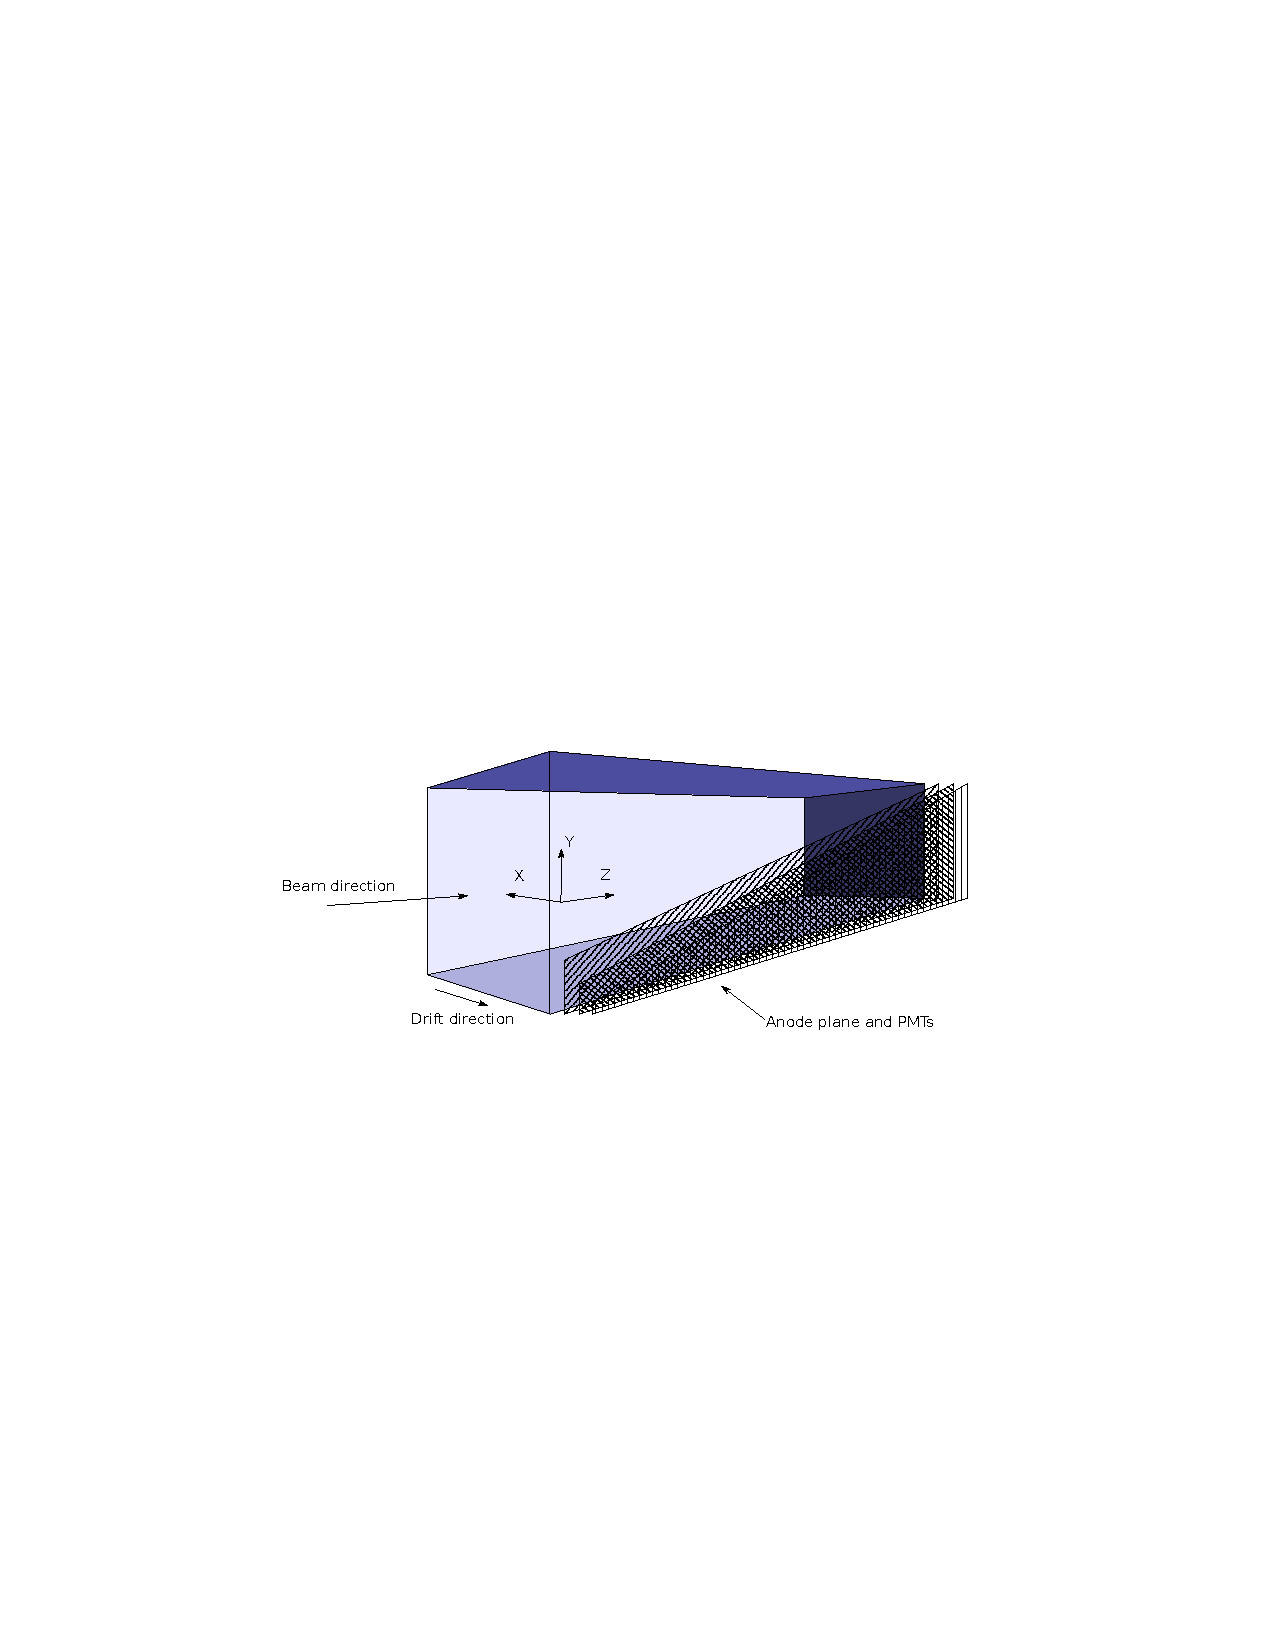
\includegraphics[width=0.8\linewidth]{figures/coord.pdf}

    \caption{The MicroBooNE coordinate system. The three wire planes are vertical (collection plane) and at  $\pm60^{\circ}$ to the vertical (induction planes). The dimensions of the TPC are 256 cm $\times$ 233 cm $\times$ 1036 cm (x $\times$ y $\times$ z). The fiducial volume of the detector is 236 cm $\times$ 203 cm $\times$ 1026 cm. The coordinate system is explained in detail in \cite{mcdata}.} \label{fig:coord}
  \end{center}
\end{figure}

This analysis has been performed on three merged datasets, acquired with different geometrical configurations. For the three different configurations, the two panels have been placed at the upstream end, at the center and at the downstream end of MicroBooNE, respectively.

A three-dimensional schematic of the three MuCS setups is shown in figure \ref{fig:mucs} and the coordinates of the two panels for each configuration are reported in Tab. \ref{tab:mucs}.
\begin{figure}[htbp]
  \begin{subfigure}{0.30\textwidth}
    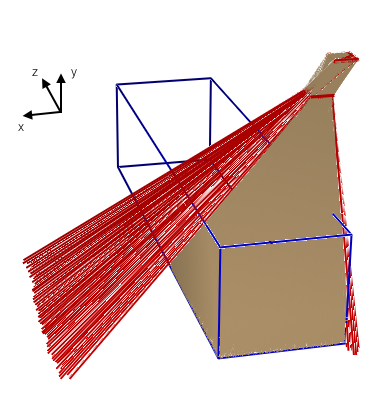
\includegraphics[width=\linewidth]{figures/upstream.png}
    \caption{Upstream} \label{fig:upstream}
  \end{subfigure}
  \begin{subfigure}{0.30\textwidth}
    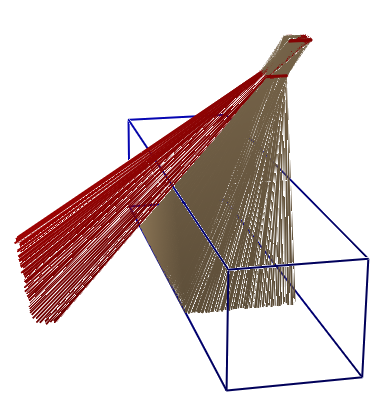
\includegraphics[width=\linewidth]{figures/center.png}
    \caption{Center} \label{fig:centre}
  \end{subfigure}
  \begin{subfigure}{0.30\textwidth}
    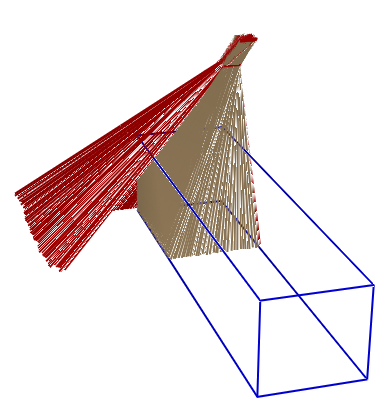
\includegraphics[width=\linewidth]{figures/downstream.png}
    \caption{Downstream} \label{fig:downstream}
  \end{subfigure}

  \caption{Monte Carlo simulation of the possible MuCS trajectories in the three different MuCS setups used in this analysis. Brown tracks correspond to cosmic rays hitting both MuCS panels and the TPC, while red tracks go through only the MuCS and miss the TPC.} \label{fig:mucs}
\end{figure}

\begin{table}[htbp]
  \centering
  \begin{tabular}{lcrrrccccc}
    \toprule
    \textbf{Configuration} & \phantom{abc}& \multicolumn{2}{c}{x [cm]} & \phantom{abc} & \multicolumn{2}{c}{y [cm]} & \phantom{abc} & \multicolumn{2}{c}{z [cm]}\\
    \cmidrule{3-4} \cmidrule{6-7} \cmidrule{9-10}
    & & start & end & & start & end & & start & end\\
    \midrule

    \textbf{Upstream} & & & & & & & & & \\
    Top panel & & -75 & -27 & & 392 & 393 & & 224 & 272\\
    Bottom panel & & -27 & 21 & & 320 & 321 & & 224 & 272\\

    \midrule
    \textbf{Center} & & & & & & & & & \\
    Top panel & & -72 & -24 & & 397 & 398 & & 579 & 627\\
    Bottom panel & & -27 & 21 & & 320 & 321 & & 581 & 629\\
    \midrule
    \textbf{Downstream} & & & & & & & & & \\
    Top panel & & -75 & -27 & & 392 & 393 & & 971 & 1019\\
    Bottom panel & & -27 & 21 & & 320 & 321 & & 971 & 1019\\
    \bottomrule

  \end{tabular}
  \caption{Coordinates of the top and bottom panels of the MuCS detector for three geometrical configurations, expressed in the TPC coordinate reference frame and obtained with a manual survey.}\label{tab:mucs}
\end{table}


\section{MuCS data processing}\label{sec:merging}
The MuCS is designed to provide a trigger on through-going muons that intersect two planes of scintillator strips. The trigger is propagated to the MicroBooNE trigger board to record a full TPC and PMT readout. With the MuCS trigger in place, the $t_0$ for a track associated with the MuCS is known and these tracks are useful for various detector physics and reconstruction studies.

The dataset used for this study has been collected with the DAQ configured in the trigger-readout mode: the MuCS trigger is sent to the TPC readout, while the MuCS DAQ saves the hit patterns seen in the scintillator strips.
The MuCS triggers at a rate of nearly 3 Hz.
Given a DAQ integration window of 100 ns, the accidental coincidental rate is negligible for our study. The probability that, during the same readout window (4.8 ms), another cosmic ray hits the MuCS is, given a trigger rate of 3 Hz, 0.01\% and it has also been considered negligible.

The data then follows a processing path that merges the MuCS hit patterns and extrapolated trajectory information with the TPC and PMT data stream to form a MuCS-merged dataset. A flowchart of the procedure is shown in figure \ref{fig:scheme}.

\begin{figure}[htbp]
  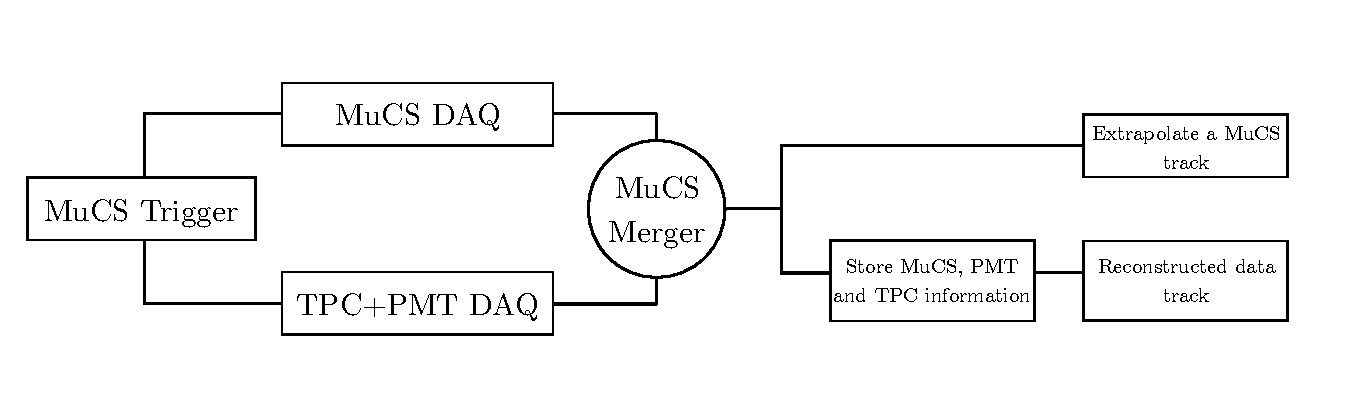
\includegraphics[width=\linewidth]{figures/scheme.pdf}
  \caption{Flowchart showing the procedure used to generate the dataset used in this analysis. We end up with two data products: one with extrapolated coordinates obtained using MuCS-only data and one with reconstructed TPC tracks and PMT flashes, if present.} \label{fig:scheme}
\end{figure}

The hits in the MuCS are used to obtain a point for each panel and extrapolate a track (MuCS-extrapolated track). The TPC hits, instead, are fed to the MicroBooNE reconstruction chain: the reconstructed track with the closest starting point to the intersection of the MuCS-extrapolated track with the TPC is stored in the dataset and it is defined as a MuCS-tagged track. The distance $d$ between these two points is defined as:
\begin{equation}\label{eq:d}
d = \sqrt{(x_{\mathrm{MuCS}}-x_{\mathrm{reco}})^2+(y_{\mathrm{MuCS}}-y_{\mathrm{reco}})^2+(z_{\mathrm{MuCS}}-z_{\mathrm{reco}})^2},
\end{equation}
where $(x_{\mathrm{MuCS}},y_{\mathrm{MuCS}},z_{\mathrm{MuCS}})$ and $(x_{\mathrm{reco}},y_{\mathrm{reco}},z_{\mathrm{reco}})$ are the coordinates of the intersection of the MuCS-extrapolated track with the TPC and of the start of the closest reconstructed track, respectively.
A PMT flash is associated with the MuCS signal if it falls between -1.0 and -0.8 \textmu s, where $t=0$ is given by the MuCS signal.
Figure \ref{fig:evd} shows a diagram with the MuCS-tagged track, the MuCS-extrapolated track and the other reconstructed tracks in the same readout window.

\begin{figure}[htbp]
  \begin{center}
  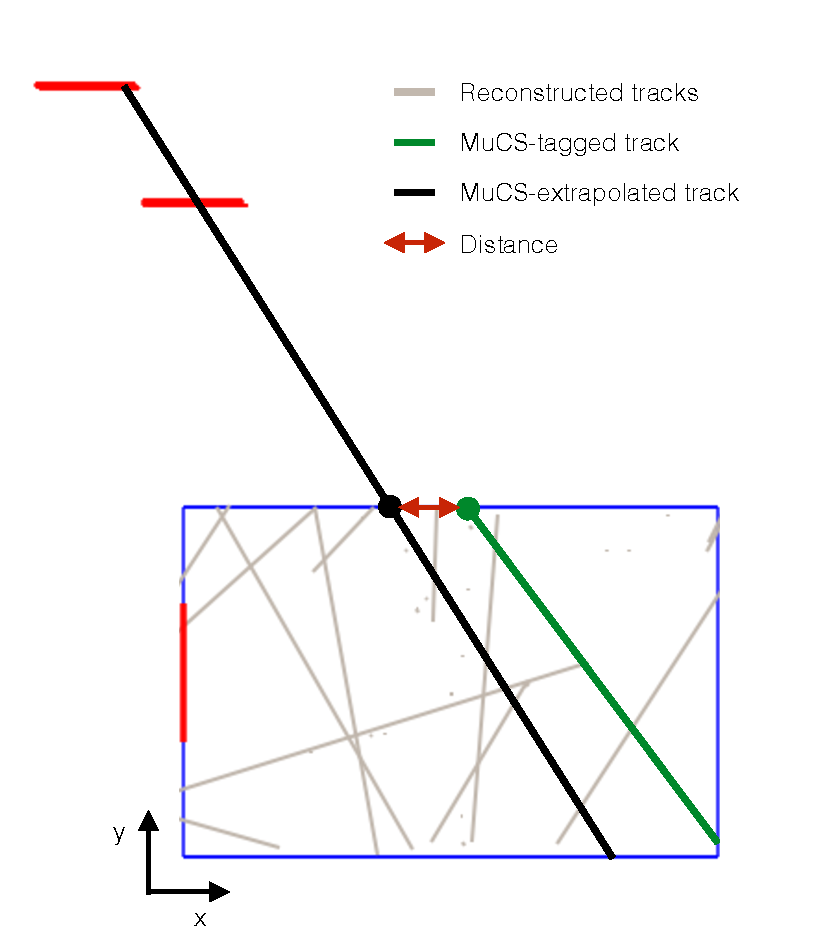
\includegraphics[width=0.50\linewidth]{figures/evd.pdf}  \vspace{1.8em}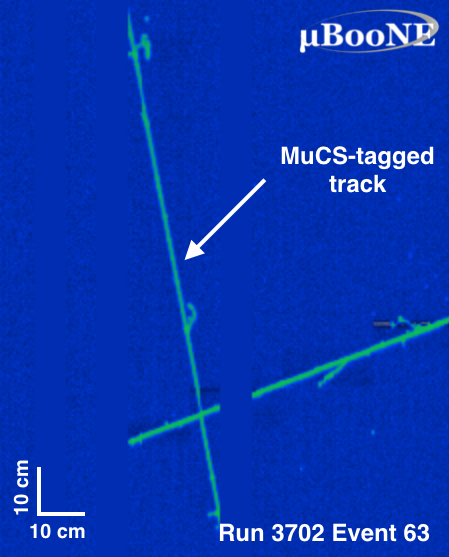
\includegraphics[width=0.40\linewidth]{figures/evd_display.png}

  \caption{Left: bi-dimensional view of a MuCS event. The black line shows the MuCS-extrapolated track, while the green line corresponds to the MuCS-tagged track. The black and green points correspond to the $(x_{\mathrm{MuCS}},y_{\mathrm{MuCS}},z_{\mathrm{MuCS}})$ and $(x_{\mathrm{reco}},y_{\mathrm{reco}},z_{\mathrm{reco}})$ coordinates, respectively. The red vertical line on the left border corresponds to the position of the PMT flash associated to the MuCS-tagged track. Right: corresponding portion of the event display for the collection plane, showing the MuCS-tagged track.} \label{fig:evd}
\end{center}
\end{figure}

Our dataset will then include two different sets of information, with a one-to-one correspondence:
\begin{itemize}
  \item MuCS-extrapolated information: using the two points given by the MuCS (one for each panel) we extrapolate a line crossing the entire TPC. In this way we obtain two extrapolated starting angles ($\theta$ and $\phi$), an extrapolated track length $L$ and extrapolated start/end points, using only MuCS information.
  \item Reconstructed TPC data information: for each event, we store the reconstructed spatial information of the MuCS-tagged track and of the in-time PMT flash, if present.
\end{itemize}

\subsection{Monte Carlo simulation}
As Monte Carlo sample we used a complete MCC7 cosmic-ray simulation, as described in \cite{cosmic}. The cosmic rays have been generated using CORSIKA \cite{corsika},  propagated with GEANT4 \cite{geant}, and then passed through the detector simulation stage. The detector simulation attempts to simulate the detector response as precisely as possible, meaning that the current state of the detector is reflected, including known unresponsive and noisy wires. Other known effects, such as the space charge effect \cite{sce}, are not currently modeled in the simulation.

The spherical angles $\theta$ and $\phi$ are measured using the starting point in the TPC and direction of the generated cosmic ray, while the expected track length $L$ is measured extrapolating a line through the TPC.

From this complete Monte Carlo simulation, then, we selected only the cosmic rays with a starting angle $(\theta,\phi)$ within the geometrical acceptance of the MuCS.

Our aim is to show that the reconstruction efficiency of simulated cosmic rays, generated all over the TPC, can be successfully compared to the data reconstruction efficiency, obtained placing a small muon counter system in three different places.

\section{MuCS alignment and angular checks}\label{sec:flux}
Before measuring the reconstruction efficiency, we performed a calibration of the position of the MuCS panels in each configuration. Taking the starting point and starting direction of the MuCS-tagged tracks it is possible to extrapolate their trajectory up to the height of the panels and check if they went through their borders. However, the build-up of positive argon ions in the TPC causes a distortion in the electric field and consequently in the reconstruction of the tracks. Thus, before measuring the starting angles and extrapolating the trajectories, the starting position and direction of the reconstructed tracks in the TPC have been corrected with the data-driven procedure described in \cite{sce}.

The two-dimensional plots of the extrapolated positions are reported in figure \ref{fig:alignment}. As we can see, some tracks are extrapolated outside the panels, because of multiple Coulomb scattering, but the majority of the points are well within the panels' borders.

\begin{figure}[htbp]
  \begin{subfigure}{0.32\textwidth}
    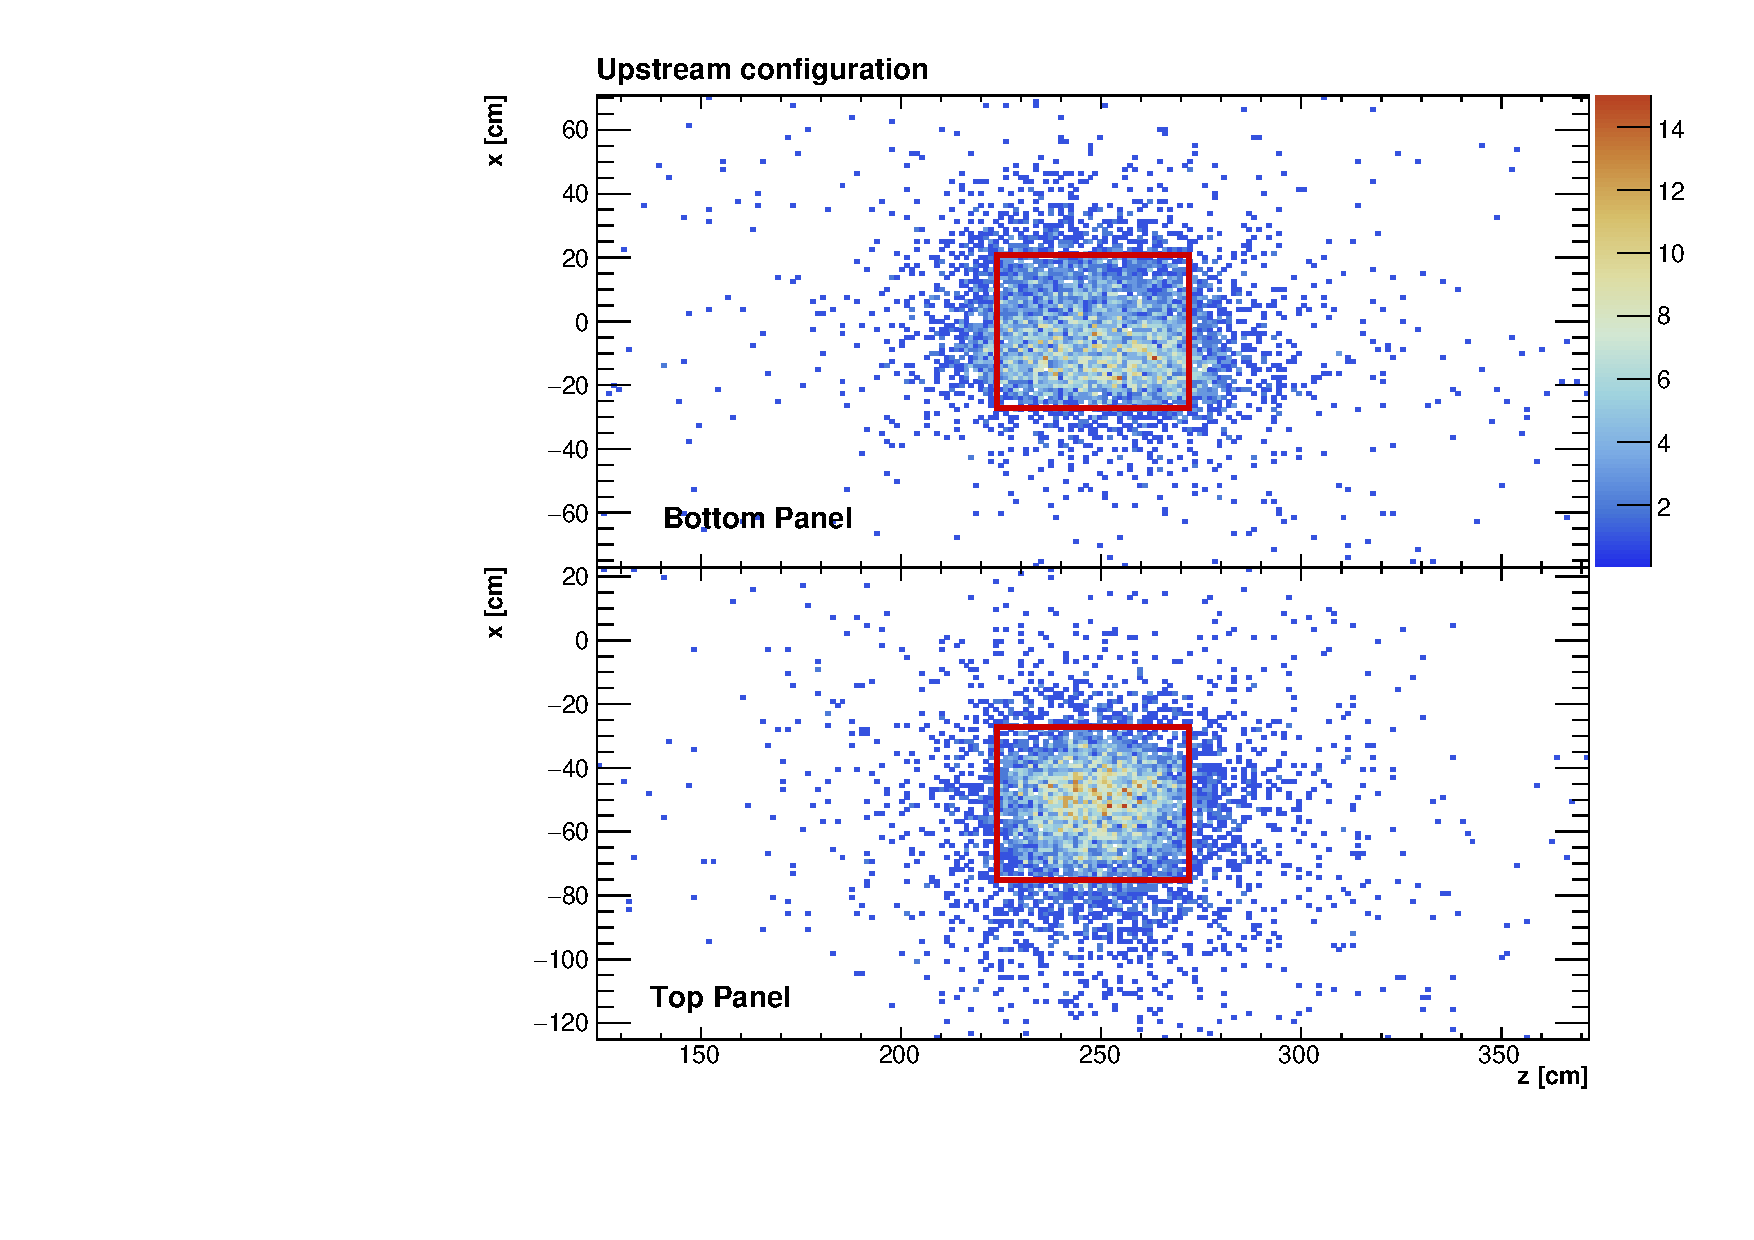
\includegraphics[width=\linewidth]{figures/upstream.pdf}
    \caption{Upstream} \label{fig:upstream_align}
  \end{subfigure}
  \begin{subfigure}{0.32\textwidth}
    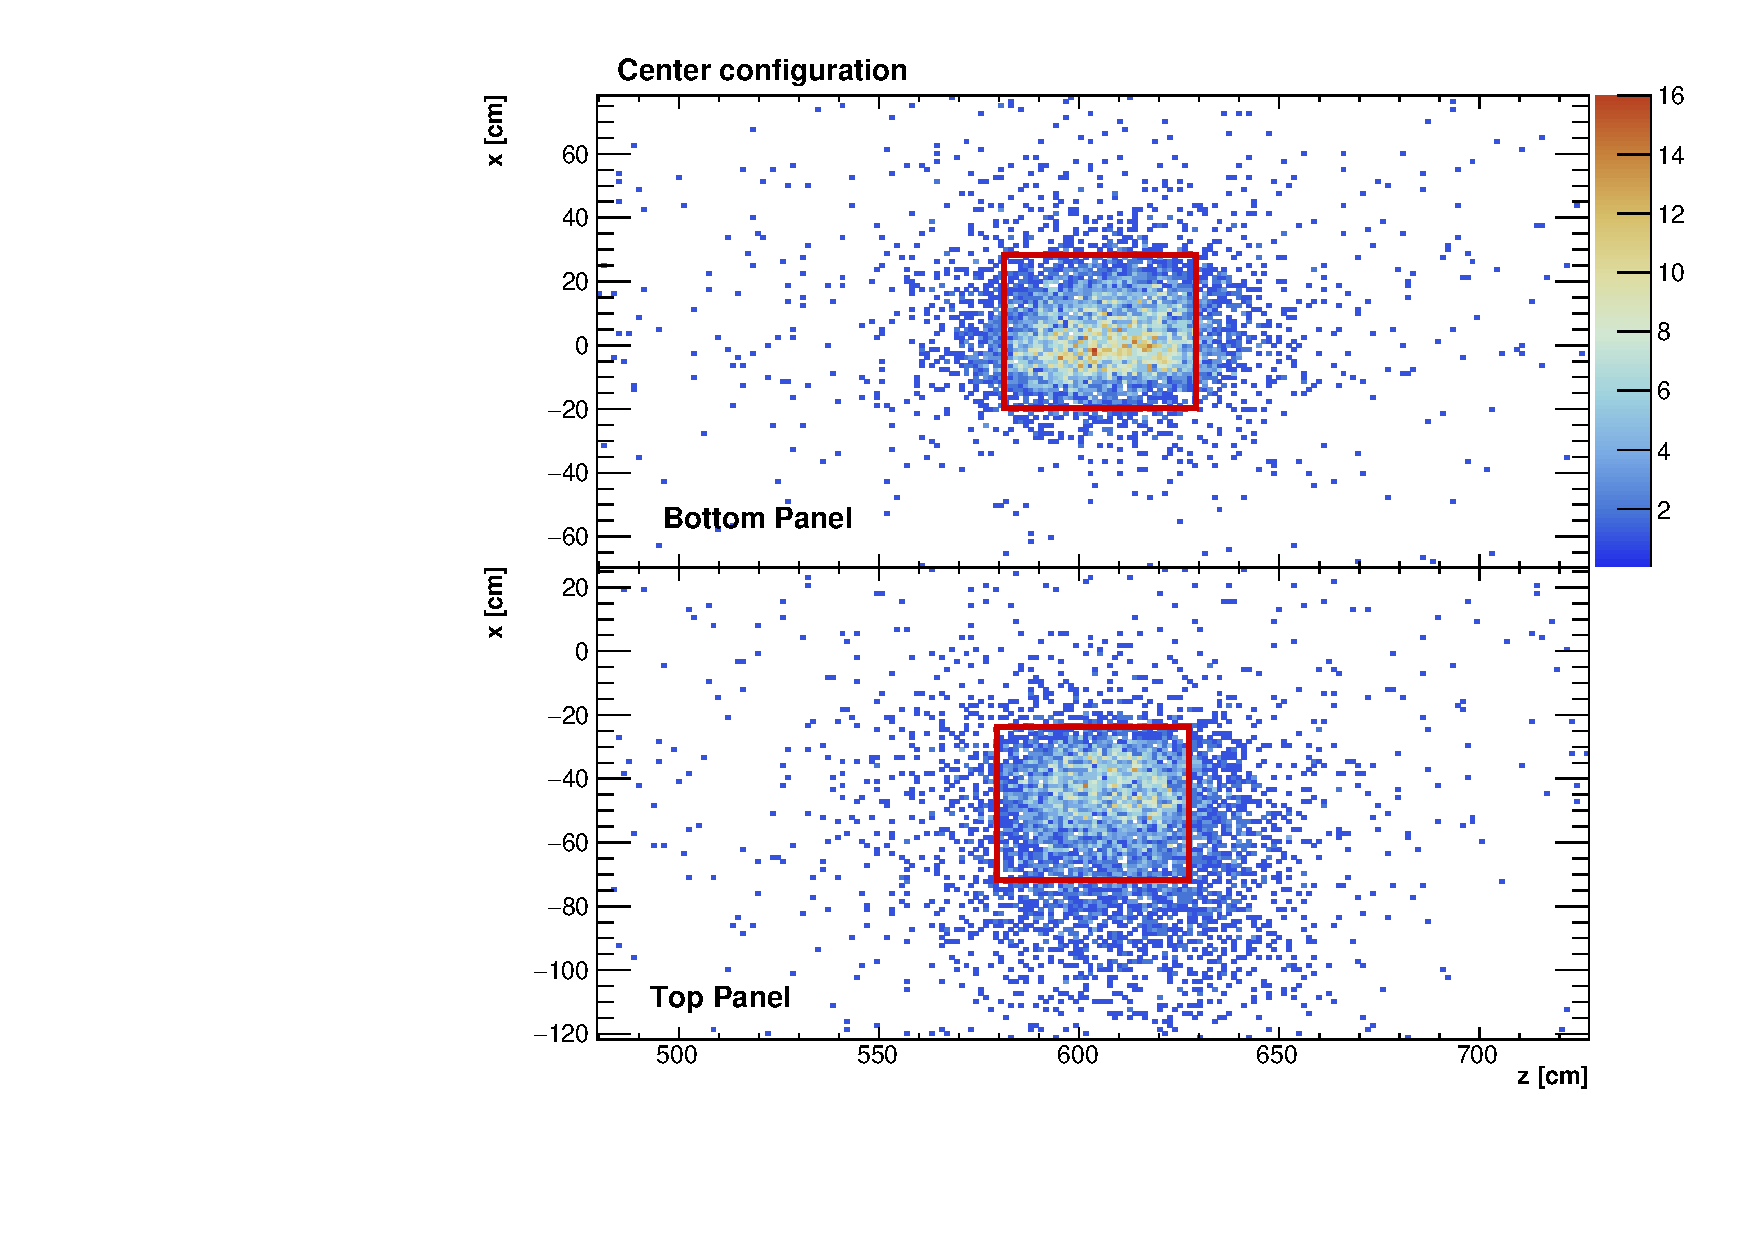
\includegraphics[width=\linewidth]{figures/centre.pdf}
    \caption{Center} \label{fig:centre_align}
  \end{subfigure}
  \begin{subfigure}{0.32\textwidth}
    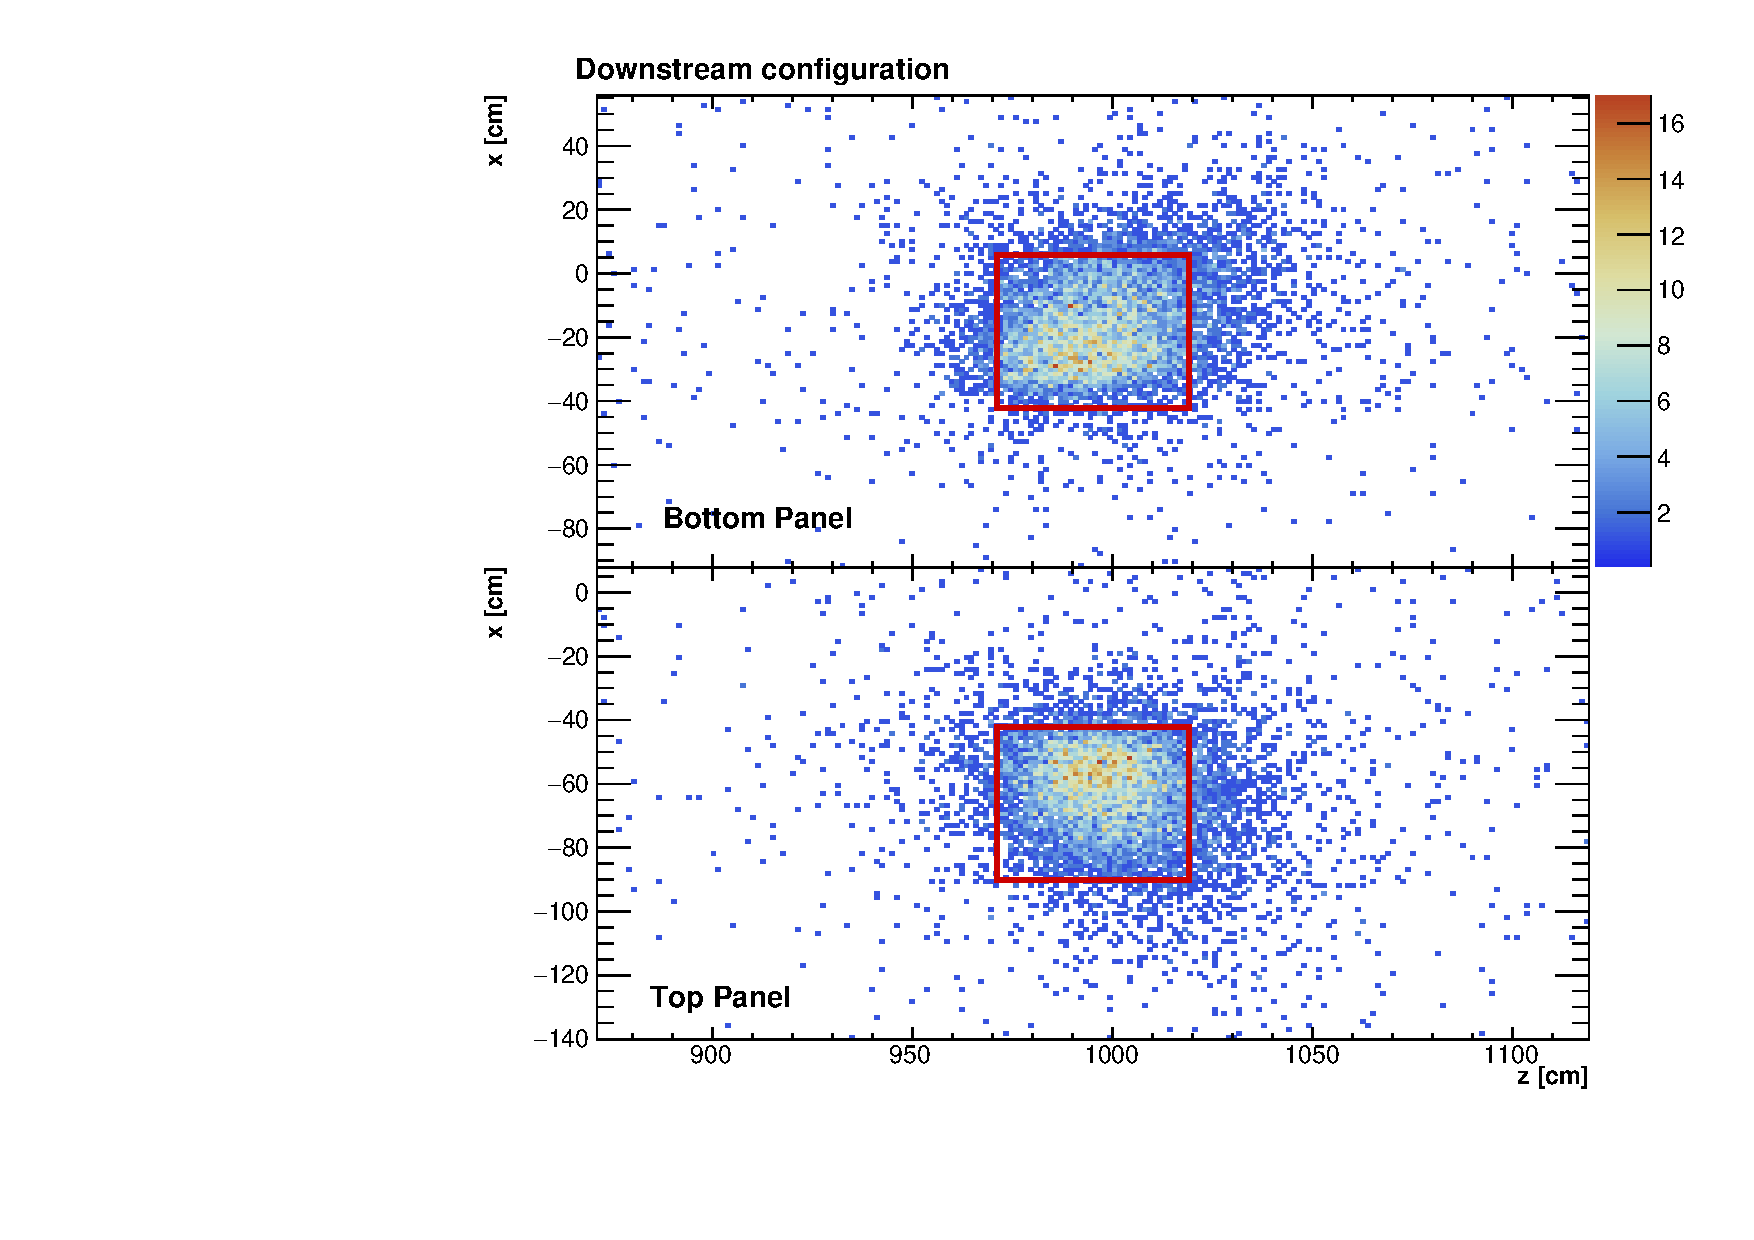
\includegraphics[width=\linewidth]{figures/downstream.pdf}
    \caption{Downstream} \label{fig:downstream_align}
  \end{subfigure}

  \caption{Extrapolated points of the MuCS-tagged tracks at the height of top and bottom panels for the upstream, center, and downstream configuration.} \label{fig:alignment}
\end{figure}

The angular distribution of the MuCS-triggering cosmic rays, obtained extrapolating a line from the MuCS hits, has been measured from the merged dataset of the three configurations and compared with an independent MuCS Monte Carlo simulation, used to check that the angular distribution of the cosmic rays was the same.  In this case, the Monte Carlo samples have been obtained generating a sample of cosmic rays within the top panel borders. Each event is stored only if the cosmic ray crosses also the bottom panel. MuCS panels have not been explicitly included in the GEANT4 stage of the simulation. This Monte Carlo information must not be confused with the reconstructed Monte Carlo information described in section \ref{sec:merging}, which is obtained reconstructing all the simulated cosmic rays in a full readout window. Figure \ref{fig:mucs_angles} shows that the distributions of the spherical angles have a good data/Monte Carlo agreement.

\begin{figure}[htbp]
  \begin{subfigure}{0.52\textwidth}
    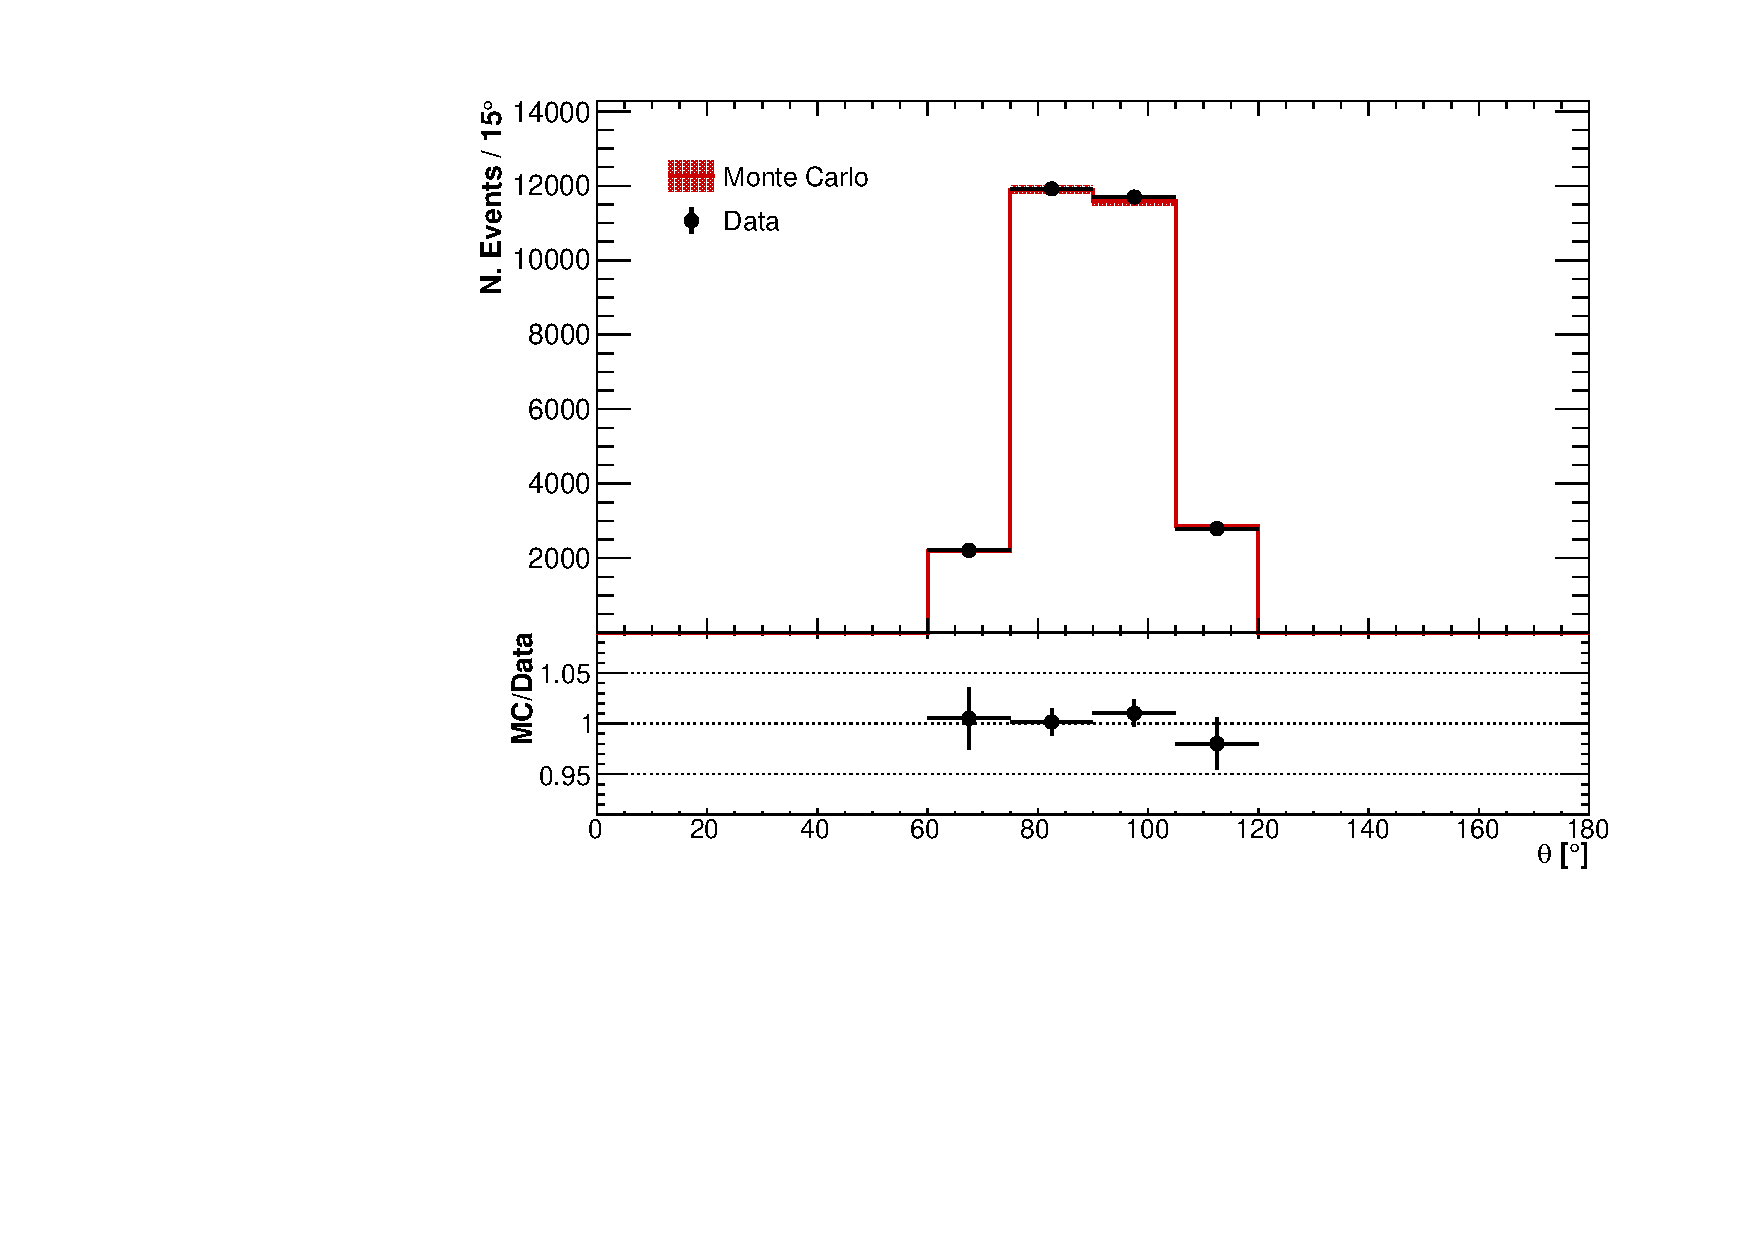
\includegraphics[width=\linewidth]{figures/theta_mucs.pdf}
    \caption{$\theta$ Data/Monte Carlo distribution.} \label{fig:theta_mucs}
  \end{subfigure}
  \begin{subfigure}{0.52\textwidth}
    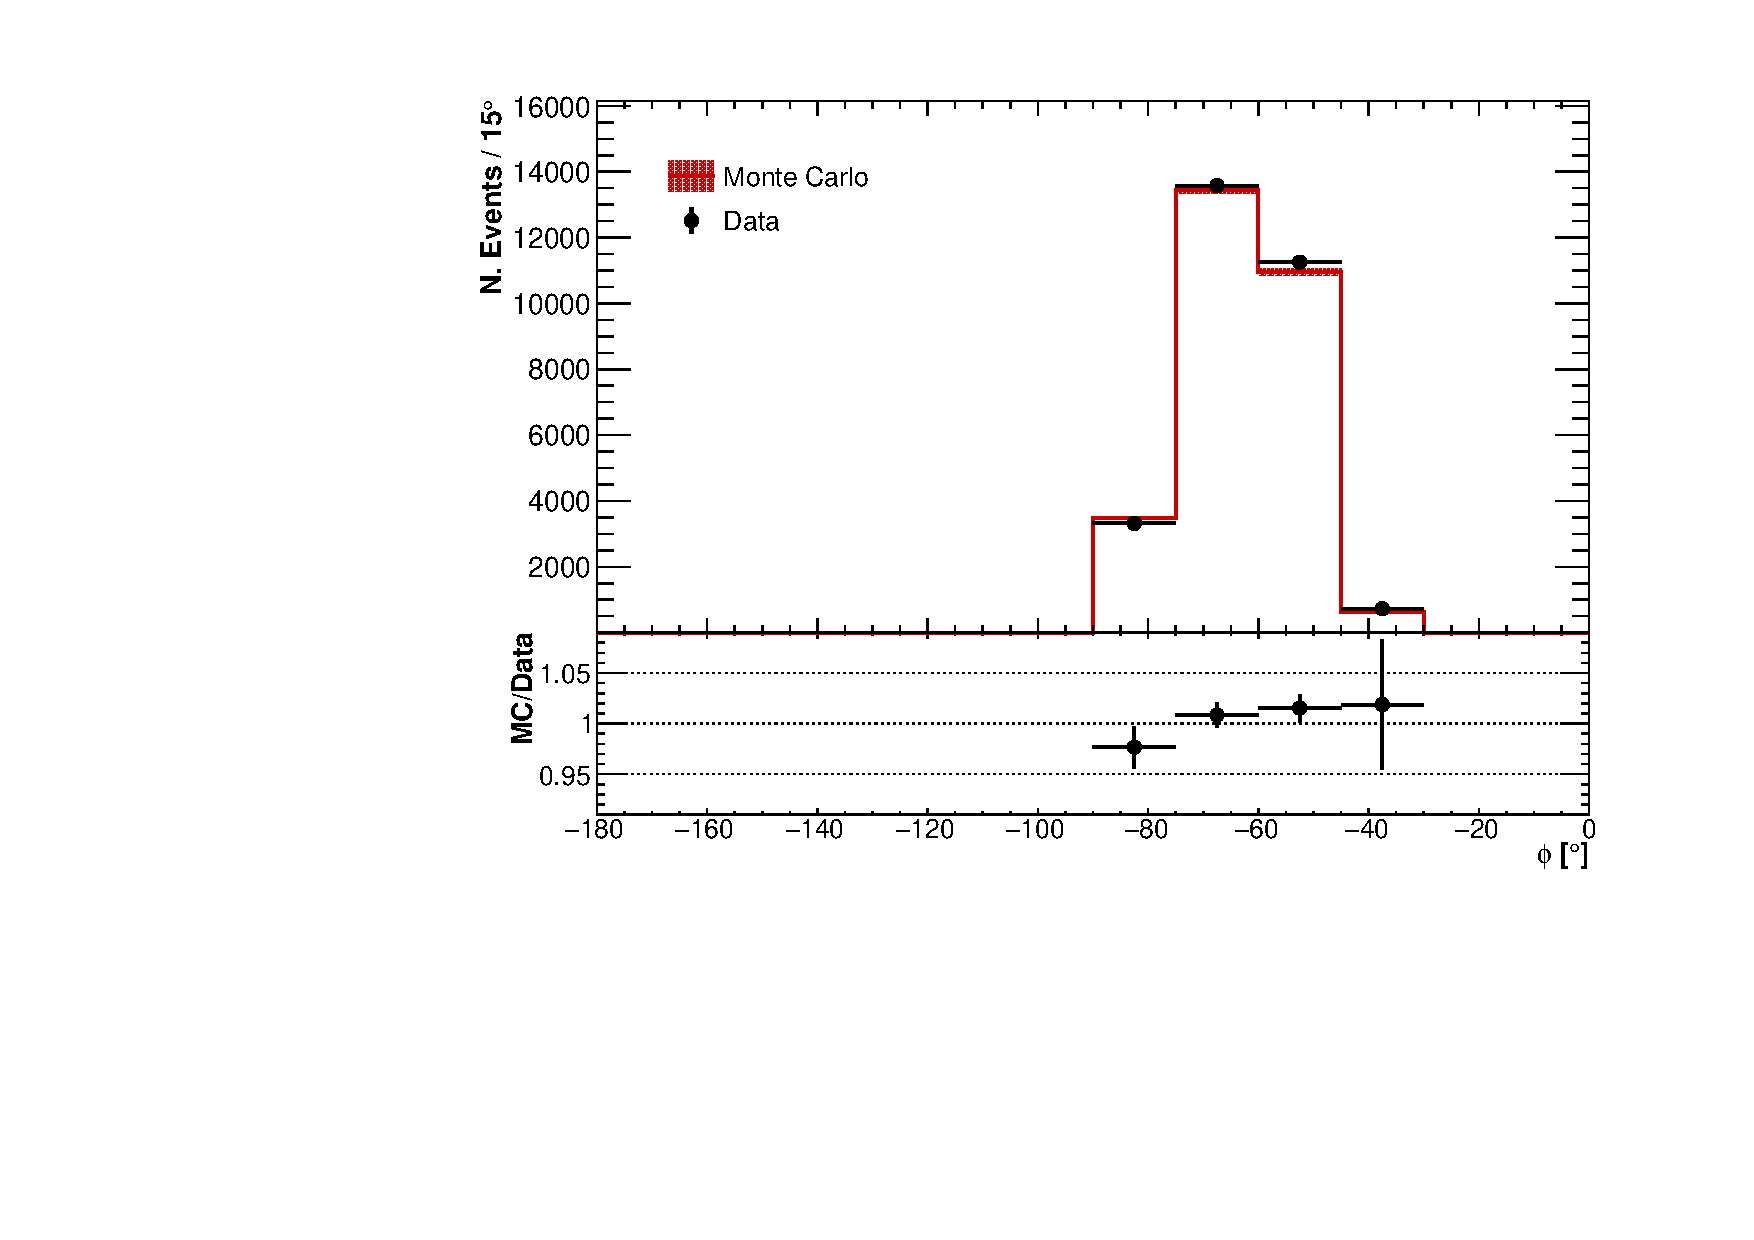
\includegraphics[width=\linewidth]{figures/phi_mucs.pdf}
    \caption{$\phi$ Data/Monte Carlo distribution.} \label{fig:phi_mucs}
  \end{subfigure}
  \caption{Data/Monte Carlo distributions of the spherical angles of the cosmic rays hitting the MuCS. Data angles have been obtained extrapolating the MuCS hits. Monte Carlo distributions have been shape-normalized to the data distributions. Errors are statistical only.} \label{fig:mucs_angles}


\end{figure}


\section{Reconstruction efficiencies}\label{sec:reco}

We define the MuCS reconstruction efficiency $\epsilon$ as the ratio between the number of events with a reconstructed MuCS cosmic ray and the number of MuCS-triggered events:
\begin{equation}\label{eq:eff}
  \epsilon = \frac{\mathrm{N.~of~reco.~MuCS~cosmic\myhyphen ray~events}}{\mathrm{N.~of~MuCS~triggered~events}}.
\end{equation}
However, in a data sample it is not possible to distinguish a MuCS cosmic ray from a normal cosmic ray and we define the MuCS-tagged track as the reconstructed track with the closest starting point $(x_{\mathrm{reco}},y_{\mathrm{reco}},z_{\mathrm{reco}})$ to the extrapolated MuCS starting point $(x_{\mathrm{MuCS}},y_{\mathrm{MuCS}},z_{\mathrm{MuCS}})$, see figure \ref{fig:evd}. Since some cosmic rays can trigger the MuCS without hitting the TPC (see red tracks in figure \ref{fig:mucs}), we keep only the events with an extrapolated trajectory in the TPC longer than 20 cm.

Events without a reconstructed MuCS cosmic ray will always have at least another reconstructed cosmic ray, so it is necessary to set a maximum distance $d_{\mathrm{max}}$ between the two points, $(x_{\mathrm{reco}},y_{\mathrm{reco}},z_{\mathrm{reco}})$ and $(x_{\mathrm{MuCS}},y_{\mathrm{MuCS}},z_{\mathrm{MuCS}})$. The number of our events with a MuCS-tagged track will then depend on $d_{\mathrm{max}}$.

In a Monte Carlo simulation of a MuCS run, generated as described in section \ref{sec:flux}, the truth information allows us to verify if the MuCS-tagged cosmic ray is a real MuCS cosmic ray, or if it is another reconstructed cosmic ray, which happens to be mis-identified due to the extrapolated starting point distance being closer than $d_{\mathrm{max}}$.
The distance $d$ is defined in this case as:
\begin{equation}\label{eq:d_mc}
d = \sqrt{(x_{\mathrm{sim}}-x_{\mathrm{reco}})^2+(y_{\mathrm{sim}}-y_{\mathrm{reco}})^2+(z_{\mathrm{sim}}-z_{\mathrm{reco}})^2},
\end{equation}
where $(x_{\mathrm{sim}},y_{\mathrm{sim}},z_{\mathrm{sim}})$ and $(x_{\mathrm{reco}},y_{\mathrm{reco}},z_{\mathrm{reco}})$ are the coordinates of the intersection of the simulated cosmic-ray trajectory with the TPC and of the closest reconstructed track, respectively. In the MuCS reconstruction efficiency definition, eq. \eqref{eq:eff}, we need then to replace the number of MuCS-triggered events with the number of simulated MuCS events.

The efficiency $\epsilon_{\mathrm{tag}}$ of the cut on $d_{\mathrm{max}}$ is defined as:
\begin{equation}
  \epsilon_{\mathrm{tag}}=\frac{\mathrm{N.~of~reco.~events~within~}d_{\mathrm{max}}}{\mathrm{N.~of~MuCS~triggered~events}}
\end{equation}
and can be measured both for our data sample ($\epsilon^{\mathrm{data}}_{\mathrm{tag}}$) and for our MuCS Monte Carlo simulation ($\epsilon^{\mathrm{MuCS-MC}}_{\mathrm{tag}}$), replacing $(x_{\mathrm{MuCS}},y_{\mathrm{MuCS}},z_{\mathrm{MuCS}})$ with $(x_{\mathrm{sim}},y_{\mathrm{sim}},z_{\mathrm{sim}})$ and the number of MuCS-triggered events with the number of simulated MuCS events.

The purity $P$ of our Monte Carlo MuCS sample will be defined as the ratio between the number of events with a reconstructed MuCS cosmic ray inside the $d_{\mathrm{max}}$ cut and the number of events with a reconstructed cosmic ray inside the $d_{\mathrm{max}}$ cut (MuCS-tagged cosmic rays):
\begin{equation}
  P=\frac{\mathrm{N.~of~reco.~MuCS~cosmic\myhyphen ray~events~within~}d_{\mathrm{max}}}{\mathrm{N.~of~reco.~events~within~}d_{\mathrm{max}}}.
\end{equation}
The acceptance $A$ of our cut on $d_{\mathrm{max}}$ will be defined as the ratio between the number of events with a reconstructed MuCS cosmic ray inside the $d_{\mathrm{max}}$ cut and the total number of events with a reconstructed MuCS cosmic ray:
\begin{equation}
  A=\frac{\mathrm{N.~of~reco.~MuCS~cosmic\myhyphen ray~events~within~}d_{\mathrm{max}}}{\mathrm{N.~of~reco.~MuCS~cosmic\myhyphen ray~events}}.
\end{equation}
The MuCS reconstruction efficiency as defined in \eqref{eq:eff}, can then be obtained, both for data ($\epsilon_{\mathrm{data}}$) and for MuCS Monte Carlo ($\epsilon_{\mathrm{MuCS\myhyphen MC}}$), by:
\begin{equation}\label{eq:mceff}
  \epsilon = \epsilon_{\mathrm{tag}} \times P / A.
\end{equation}
where the $P/A$ ratio will be taken only from the MuCS Monte Carlo simulation, while $\epsilon_{\mathrm{tag}}$ can be measured with the data, $\epsilon^{\mathrm{data}}_{\mathrm{tag}}$, or with the MuCS Monte Carlo simulation, $\epsilon^{\mathrm{MuCS\myhyphen MC}}_{\mathrm{tag}}$.

Figure \ref{fig:purity} shows the tagging efficiency both for data ($\epsilon^{\mathrm{data}}_{\mathrm{tag}}$) and MuCS Monte Carlo  ($\epsilon^{\mathrm{MuCS\myhyphen MC}}_{\mathrm{tag}}$), the purity $P$ and the acceptance $A$ as a function of $d_{\mathrm{max}}$. The MuCS reconstruction efficiencies for data ($\epsilon_{\mathrm{data}}$) and Monte Carlo ($\epsilon_{\mathrm{MuCS\myhyphen MC}}$) are also shown as a reference.

\begin{figure}[htbp]
  \begin{center}
    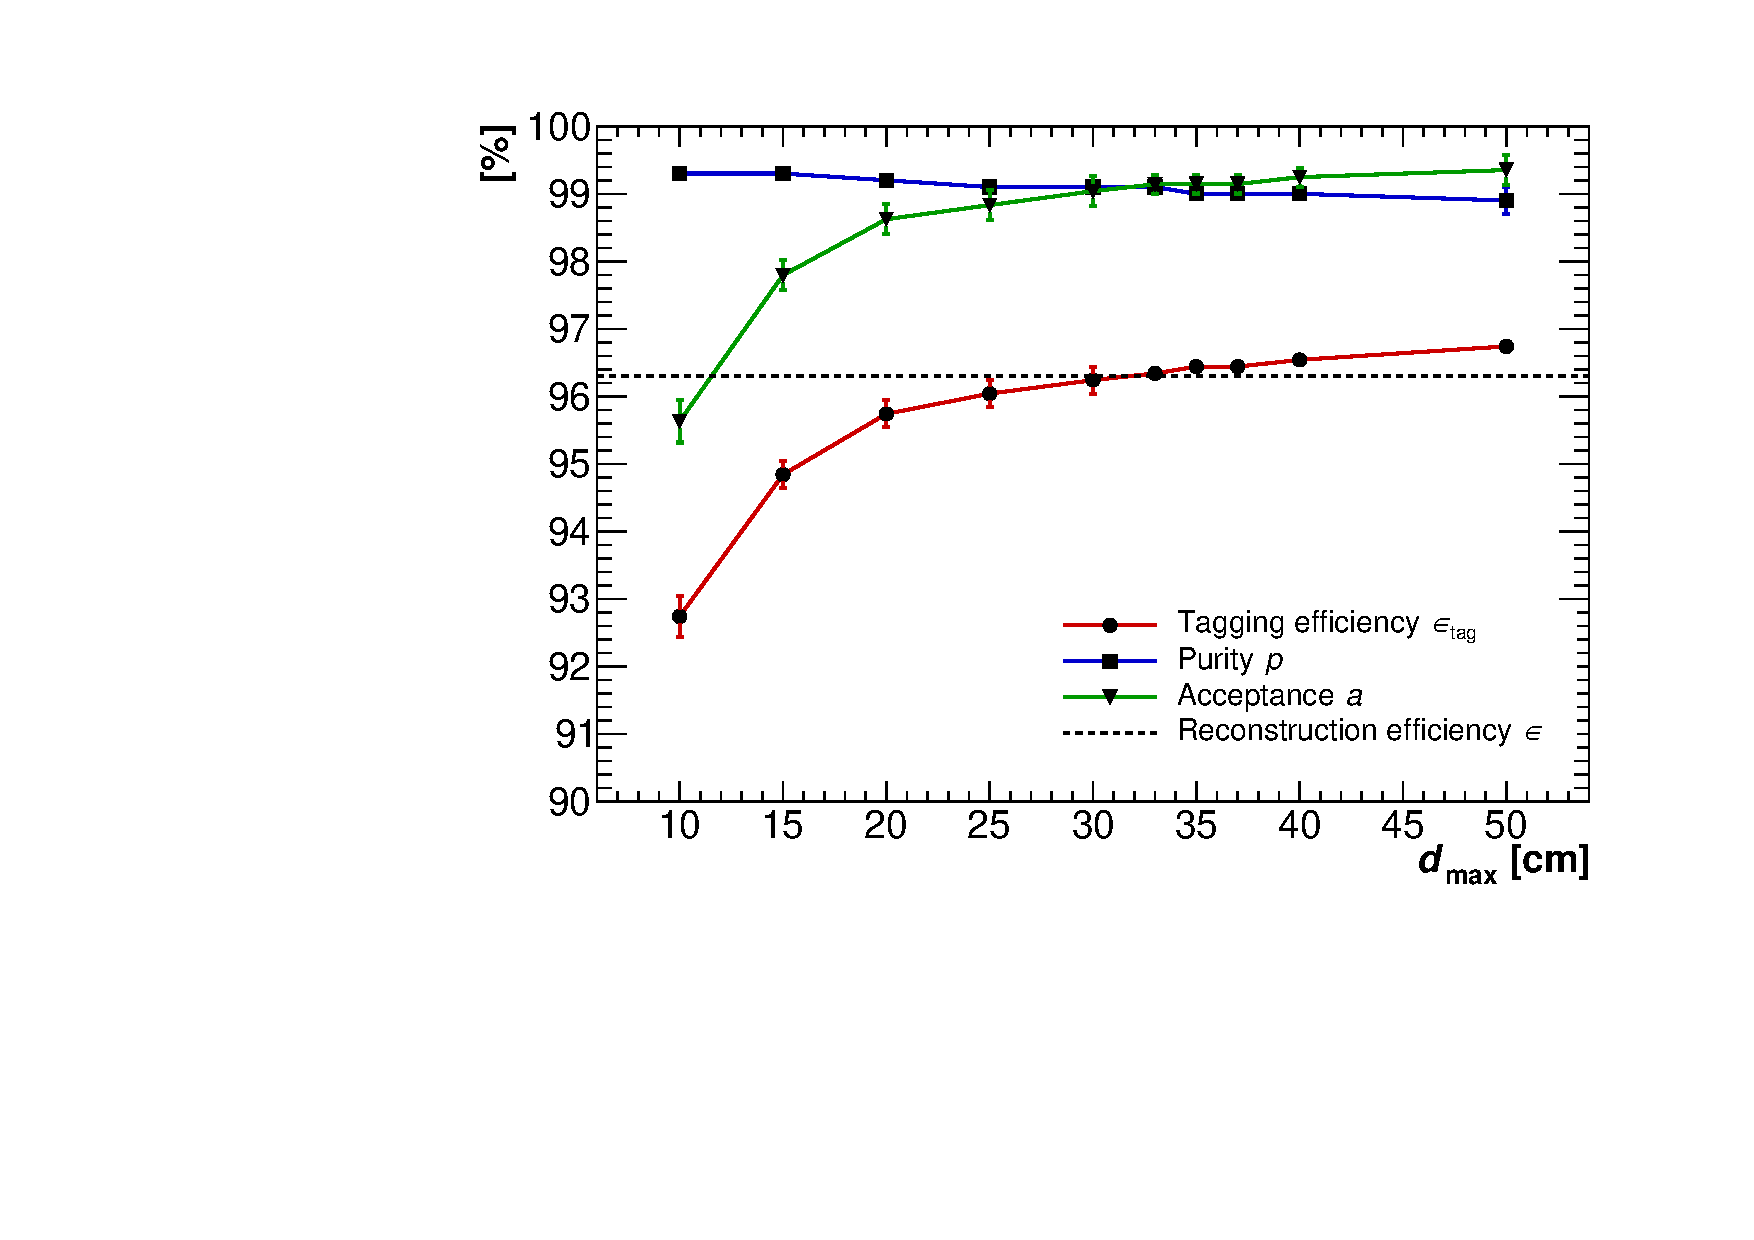
\includegraphics[width=0.7\linewidth]{figures/purity.pdf}
    \caption{Data $\epsilon^{\mathrm{data}}_{\mathrm{tag}}$ and Monte Carlo $\epsilon^{\mathrm{MC}}_{\mathrm{tag}}$ tagging efficiency (red), purity $P$ (blue) and acceptance $A$ (green) as a function of $d_{\mathrm{max}}$. The MuCS reconstruction efficiencies for data ($\epsilon_{\mathrm{data}}$) and Monte Carlo ($\epsilon_{\mathrm{MC}}$) are also shown as a reference (grey).} \label{fig:purity}
  \end{center}
\end{figure}

Using eq. \eqref{eq:eff}, our MuCS Monte Carlo reconstruction efficiency $\epsilon_{\mathrm{MuCS\myhyphen MC}}$ will not depend, by construction, on the chosen value of $d_{\mathrm{max}}$. Since the $P/A$ correcting factor has been measured with a Monte Carlo simulation, the data reconstruction efficiency $\epsilon_{\mathrm{data}}$ will have a small dependance on $d_{\mathrm{max}}$ (see figure \ref{fig:purity}), because of the small difference between $\epsilon^{\mathrm{data}}_{\mathrm{tag}}$ and $\epsilon^{\mathrm{MuCS\myhyphen MC}}_{\mathrm{tag}}$.
The difference between the lowest and the highest value of $\epsilon_{\mathrm{data}}$ is 0.2\%. This value has been used to quote the systematic uncertainty related to the $P/A$ correcting factor.
For convenience's sake, we chose a value of $d_{\mathrm{max}}$ that corresponds to $P/A = 1$, which in our case resulted to be $d_{\mathrm{max}}=32~\mathrm{cm}$.

Values of $\epsilon_{\mathrm{data}}$ and $\epsilon_{\mathrm{MuCS\myhyphen MC}}$ for each configuration are reported in Tab. \ref{tab:config}.

\begin{table}[htbp]
  \centering
  \begin{tabular}{lccccccccc}
    \toprule
    Configuration & \phantom{a} & \multicolumn{2}{c}{$\epsilon_{\mathrm{data}}$} & \phantom{a} & \multicolumn{2}{c}{$\epsilon_{\mathrm{MuCS\myhyphen MC}}$} \\
     \cmidrule{3-4} \cmidrule{6-7}
      &  & avg. & err. & & avg. & err.  \\
    \midrule
    Central & & 95.9 & 0.2 & & 96.3 & 0.1 \\
    Upstream & & 95.7 & 0.2 & & 96.0 & 0.1 \\
    Downstream & & 97.1 & 0.2 & & 97.3 & 0.1 \\
    \midrule
    Overall & & 96.1 & 0.1 & & 96.3 & 0.1 \\
    \bottomrule
  \end{tabular}
  \caption{Reconstruction efficiency for each geometrical configuration for data and MuCS Monte Carlo.}\label{tab:config}
\end{table}


The Monte Carlo cosmic-ray reconstruction efficiency, obtained with a general Monte Carlo distribution generated as described in section \ref{sec:merging}, can be directly defined as:
\begin{equation}
  \epsilon_{\mathrm{MC}} = \frac{\mathrm{N.~of~reco.~cosmic\myhyphen ray~events}}{\mathrm{N.~of~generated~cosmic\myhyphen ray~events}}.
\end{equation}

This Monte Carlo sample will contain cosmic rays generated all over the TPC, with $\epsilon_{\mathrm{MC}}$ having a minimal dependence on the position of the cosmic ray in the TPC. A direct comparison with the MuCS data will allow us to verify if the data reconstruction efficiency, measured in specific parts of the detector, is valid all over the detector.

We can express the data, $\epsilon_{\mathrm{data}}$, and the Monte Carlo, $\epsilon_{\mathrm{MC}}$, reconstruction efficiencies as a function of the spherical starting angles $\theta$, $\phi$ and of the expected track length $L$ in the TPC. In an ideal TPC, in fact, the reconstruction efficiency for a cosmic ray depends only on the number of hit wires, which is given unequivocally by the direction and the length of the track in the TPC.

Our efficiency can then be plotted as a three-dimensional histogram: each bin will correspond to a particular combination of the $\theta$, $\phi$, $L$ variables. Bin width has been chosen large enough to have at least 15 MuCS triggered events in every ($\theta$, $\phi$, $L$) bin. The same $P/A$ correction factor has been applied to every bin. Figure \ref{fig:3d} shows both the data and the Monte Carlo reconstruction efficiency, generated as described in section \ref{sec:merging}. The overall track reconstruction efficiency, obtained integrating the three-dimensional histograms and without considering systematic uncertainties is:
\begin{align*}
\epsilon_{\mathrm{data}} &= 96.1 \pm 0.1~\%\\
\epsilon_{\mathrm{MC}} &= 97.3 \pm 0.1~\%
\end{align*} for data and Monte Carlo, respectively. However, this value of $\epsilon_{\mathrm{data}}$ does not take into account muons decaying or being captured before reaching the TPC and its error is staistical only.

\begin{figure}[htbp]
  \begin{subfigure}{0.52\textwidth}
    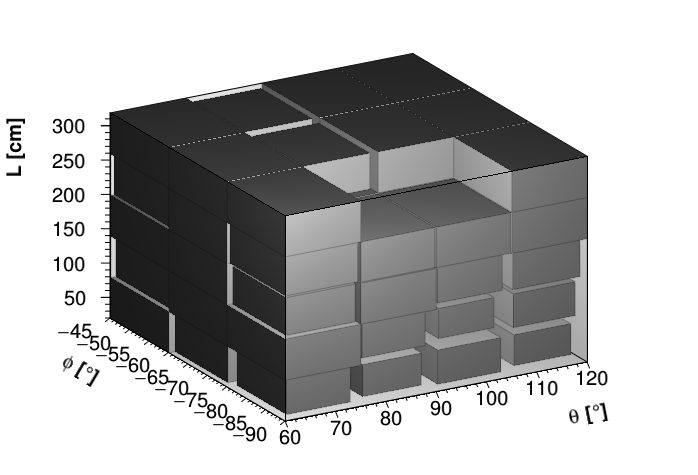
\includegraphics[width=\linewidth]{figures/3d_mc.png}
    \caption{Monte Carlo} \label{fig:3d_mc}
  \end{subfigure}
  \begin{subfigure}{0.52\textwidth}
    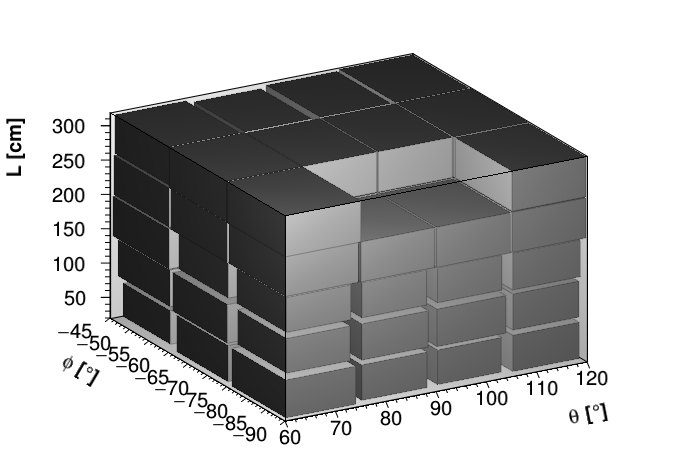
\includegraphics[width=\linewidth]{figures/3d_data.png}
    \caption{Data} \label{fig:3d_data}
  \end{subfigure}
  \caption{Monte Carlo and data three-dimensional reconstruction efficiency as a function of the starting angles $\theta$, $\phi$ and the extrapolated track length $L$. A larger box corresponds to a larger efficiency. The empty region in the upper part of the plot corresponds to a region of the parameter space not covered by our dataset.}\label{fig:3d}
\end{figure}
\section{Systematic uncertainties}
\subsection{Decay-in-flight or captured muons}\label{sec:dif}
The cosmic muons hitting the MuCS can decay in flight or being captured before reaching the LArTPC. In this case, they trigger the MuCS but do not generate a cosmic track in the detector. Since in our definition of the data reconstruction efficiency $\epsilon_{\mathrm{data}}$, eq. \eqref{eq:eff}, the denominator correspond to the number of MuCS-triggered events, we need to correct for this effect. From our MuCS Monte Carlo simulation we measured the fraction of cosmic rays that go through the MuCS but decay before reaching the LArTPC:
\begin{equation}
D = \frac{\mathrm{N.~of~decays~in~flight}}{\mathrm{N.~of~MuCS~triggered~events}} = 1.0 \pm 0.1~\%.
\end{equation}
We assume this correction factor to be independent from $\theta$, $\phi$ and $L$. The corrected data reconstruction efficiency is given by:
\begin{equation}
\epsilon_{\mathrm{data}}^{\mathrm{corr}} =  \frac{\epsilon_{\mathrm{data}}}{1-D} = 97.1\%.
\end{equation}
The statistical uncertainty of the correcting factor $D$, 0.1\%, is propagated and included in the list of the data reconstruction efficiency systematic uncertainties.

\subsection{Detector non-uniformities}\label{sec:wires}
The presence of detector non-uniformities can introduce a systematic uncertainty in the measurement of the reconstruction efficiency. In particular, the presence of noisy or unresponsive wires in specific regions of the detector can lower the reconstruction efficiency in some of our three datasets. However, the different configurations allow us to cover different regions of the TPC, providing information on potential non-uniformities.

To check if these non-uniformities introduce a systematic effect, we measured the significance $\sigma$ of the differences between the data reconstruction efficiencies measured in two different configurations with the following definition:
\begin{equation}
\sigma = \frac{\epsilon_a-\epsilon_b}{\sqrt{\Delta \epsilon_{a}^2 + \Delta \epsilon_b^2}},
\end{equation}
where $\epsilon_{a}$ ($\epsilon_{b}$) is the reconstruction efficiency in the $a$ ($b$) configuration and $\Delta \epsilon_{a}$ ($\Delta \epsilon_{b}$) is the corresponding statistical error. This significance has been measured for each $\theta,\phi,L$ bin and for each possible combination of central, downstream and upstream configuration (described in section \ref{sec:proc}). If there is a systematic effect, the standard deviation of the significances distribution should be larger than unity. In our case, as shown in figure \ref{fig:significance}, the Gaussian fit of the distribution gives $\sigma = 1.54\pm0.12$, so larger than 1.

\begin{figure}[htbp]
  \begin{center}
    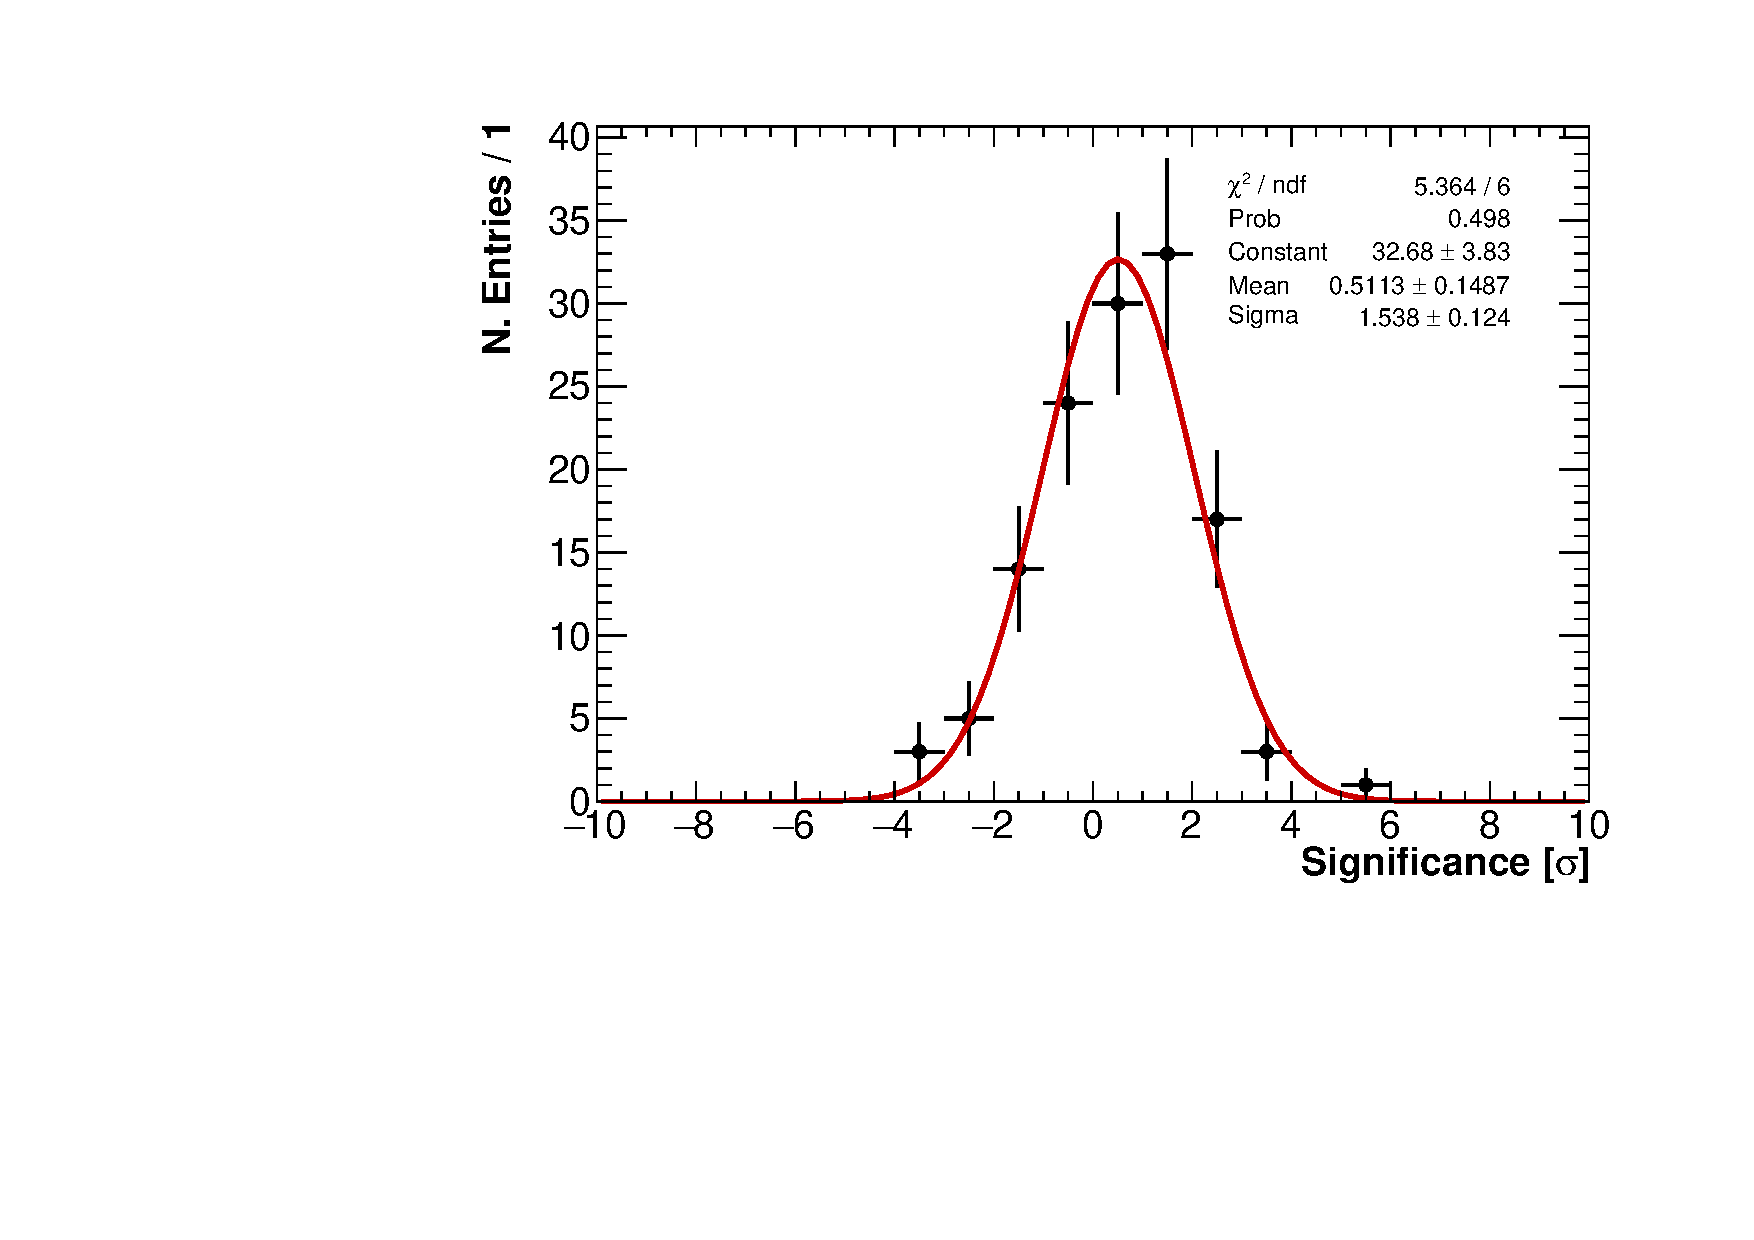
\includegraphics[width=0.7\linewidth]{figures/significance.pdf}
    \caption{Distribution of the significances of the reconstruction efficiency for each $\theta,\phi,L$ bin, measured for any combination of the three MuCS configuration.} \label{fig:significance}
  \end{center}
\end{figure}

In order to understand if these discrepancies are caused by noisy or unresponsive wires in specific parts of detector, the bins corresponding to significances larger than 3 have been reported in Tab. \ref{tab:significance}.

\begin{table}[htbp]
  \centering
  \begin{tabular}{cccccccccccc}
    \toprule
    $\theta\thinspace[^\circ]$ & $\phi\thinspace[^\circ]$ & $L\thinspace[\mathrm{cm}]$ & \phantom{a} & \multicolumn{2}{c}{Central} & \phantom{a} & \multicolumn{2}{c}{Upstream} & \phantom{a} & \multicolumn{2}{c}{Downstream}\\
     \cmidrule{5-6} \cmidrule{8-9} \cmidrule{11-12}
      &  &  & & avg. & err. & & avg. & err. & & avg. & err.   \\
    \midrule
    75 & -60 & 20 & & \textbf{0.85} & \textbf{0.04} & & \textbf{0.85} & \textbf{0.02} & & 0.95 & 0.02\\
    90 & -90 & 140 & & 0.97 & 0.03 & & \textbf{0.70} & \textbf{0.07} & & 0.93 & 0.04\\
    90 & -90 & 200 & & 0.99 & 0.01 & & \textbf{0.96} & \textbf{0.01} & & 0.99 & 0.01\\
    90 & -60 & 140 & & 0.98 & 0.01 & & \textbf{0.96} & \textbf{0.01} & & 0.99 & 0.01\\
    90 & -60 & 200 & & 0.99 & 0.01 & & \textbf{0.96} & \textbf{0.01} & & 0.89 & 0.01\\

    \bottomrule
  \end{tabular}
  \caption{Reconstruction efficiency for each geometrical configuration with a difference significance larger than 3. The lowest value is reported in bold.}\label{tab:significance}
\end{table}

As we can see, the configuration with the lowest reconstruction efficiency in this cases is always the upstream one. The drawing of the extrapolated tracks with those specific $\theta,\phi,L$ coordinates shows that, for the upstream configuration, the corresponding cosmic rays go through regions with noisy or unresponsive wires in one of the induction planes (figure \ref{fig:wires}).

\begin{figure}[htbp]
  \begin{center}
    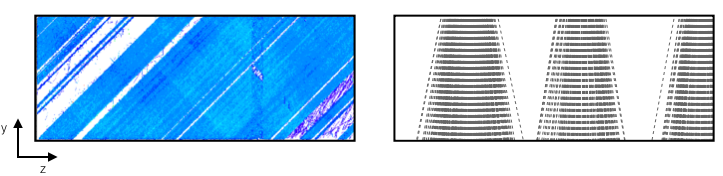
\includegraphics[width=1\linewidth]{figures/wire_tracks.png}
    \caption{Bi-dimensional plot of the collected charge, showing the regions with missing wires on one of the induction planes (left) and extrapolated tracks corresponding to the coordinates in Tab. \ref{tab:significance} (right). As we can see, the tracks in the upstream part of the detector (low $z$) go through a region with several missing wires.} \label{fig:wires}
  \end{center}
\end{figure}


Moreover, since their $\theta$ angle is close to $90^\circ$, they are also aligned with the wires of the collection plane. Thus, these cosmic rays have few hits in two of the three planes and the algorithm is not efficient to reconstruct a track. Figure \ref{fig:example} shows a non-reconstructed MuCS cosmic ray going through the region with missing wires and parallel to the collection plane wires.

\begin{figure}[htbp]
  \begin{center}
    \begin{subfigure}{0.3\textwidth}
      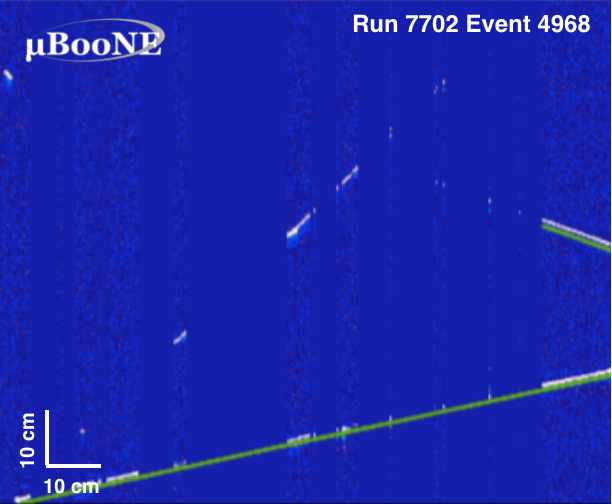
\includegraphics[width=\linewidth]{figures/u.png}
      \caption{Induction (U) plane} \label{fig:u}
    \end{subfigure}
    \begin{subfigure}{0.3\textwidth}
      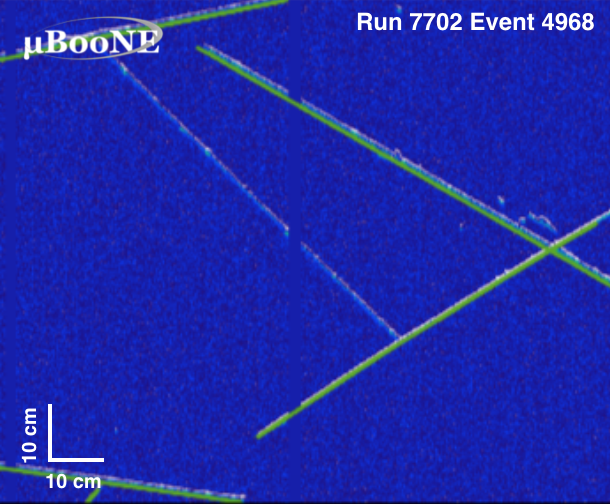
\includegraphics[width=\linewidth]{figures/v.png}
      \caption{Induction (V) plane} \label{fig:v}
    \end{subfigure}
    \begin{subfigure}{0.3\textwidth}
      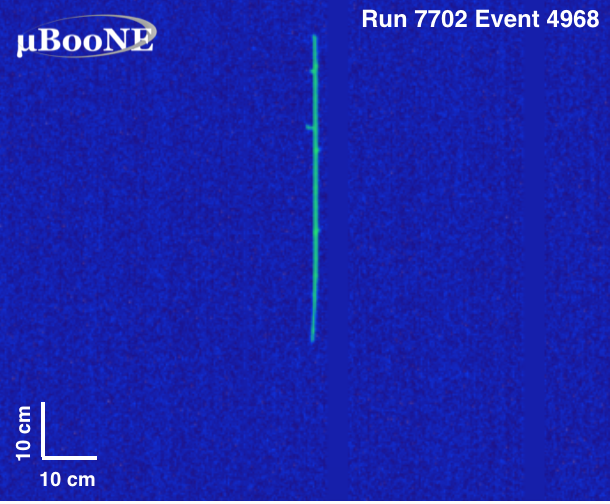
\includegraphics[width=\linewidth]{figures/y.png}
      \caption{Collection (Y) plane} \label{fig:y}
    \end{subfigure}    \caption{Event display of a non-reconstructed MuCS cosmic-ray track in the U, V and Y planes. Green lines correspond to the reconstructed tracks.} \label{fig:example}
  \end{center}
\end{figure}

We quote the systematic uncertainty related to the detector non-uniformities for each $\theta,\phi,L$ bin as the difference between the best reconstruction efficiency of the three configurations and the overall reconstruction efficiency (obtained merging the three dataset), a method described in \cite{besiii}. The overall systematic uncertainty resulted to be 1.1\%, that is the difference between the overall reconstruction efficiency of the best configuration and the overall reconstruction efficiency of the merged sample.

\subsection{Energy sampling}
The multiple Coulomb scattering depends on the energy of the cosmic ray. The angular dispersion $\theta_{0}$ of a cosmic muon can be, in fact, calculated by the relation, expressed in \cite{pdg}:
\begin{equation}
\theta_{0} = \frac{13.6~\mathrm{MeV}}{\beta c p}\sqrt{x/X_{0}}\left[1+0.038\thinspace\mathrm{ln}(x/X_0)\right],
\end{equation}
where $p$ and $\beta c$ are the momentum and velocity of the incident particle, and $x/X_0$ is the thickness of the scattering medium in radiation lengths.

\begin{figure}[htbp]
  \begin{center}
    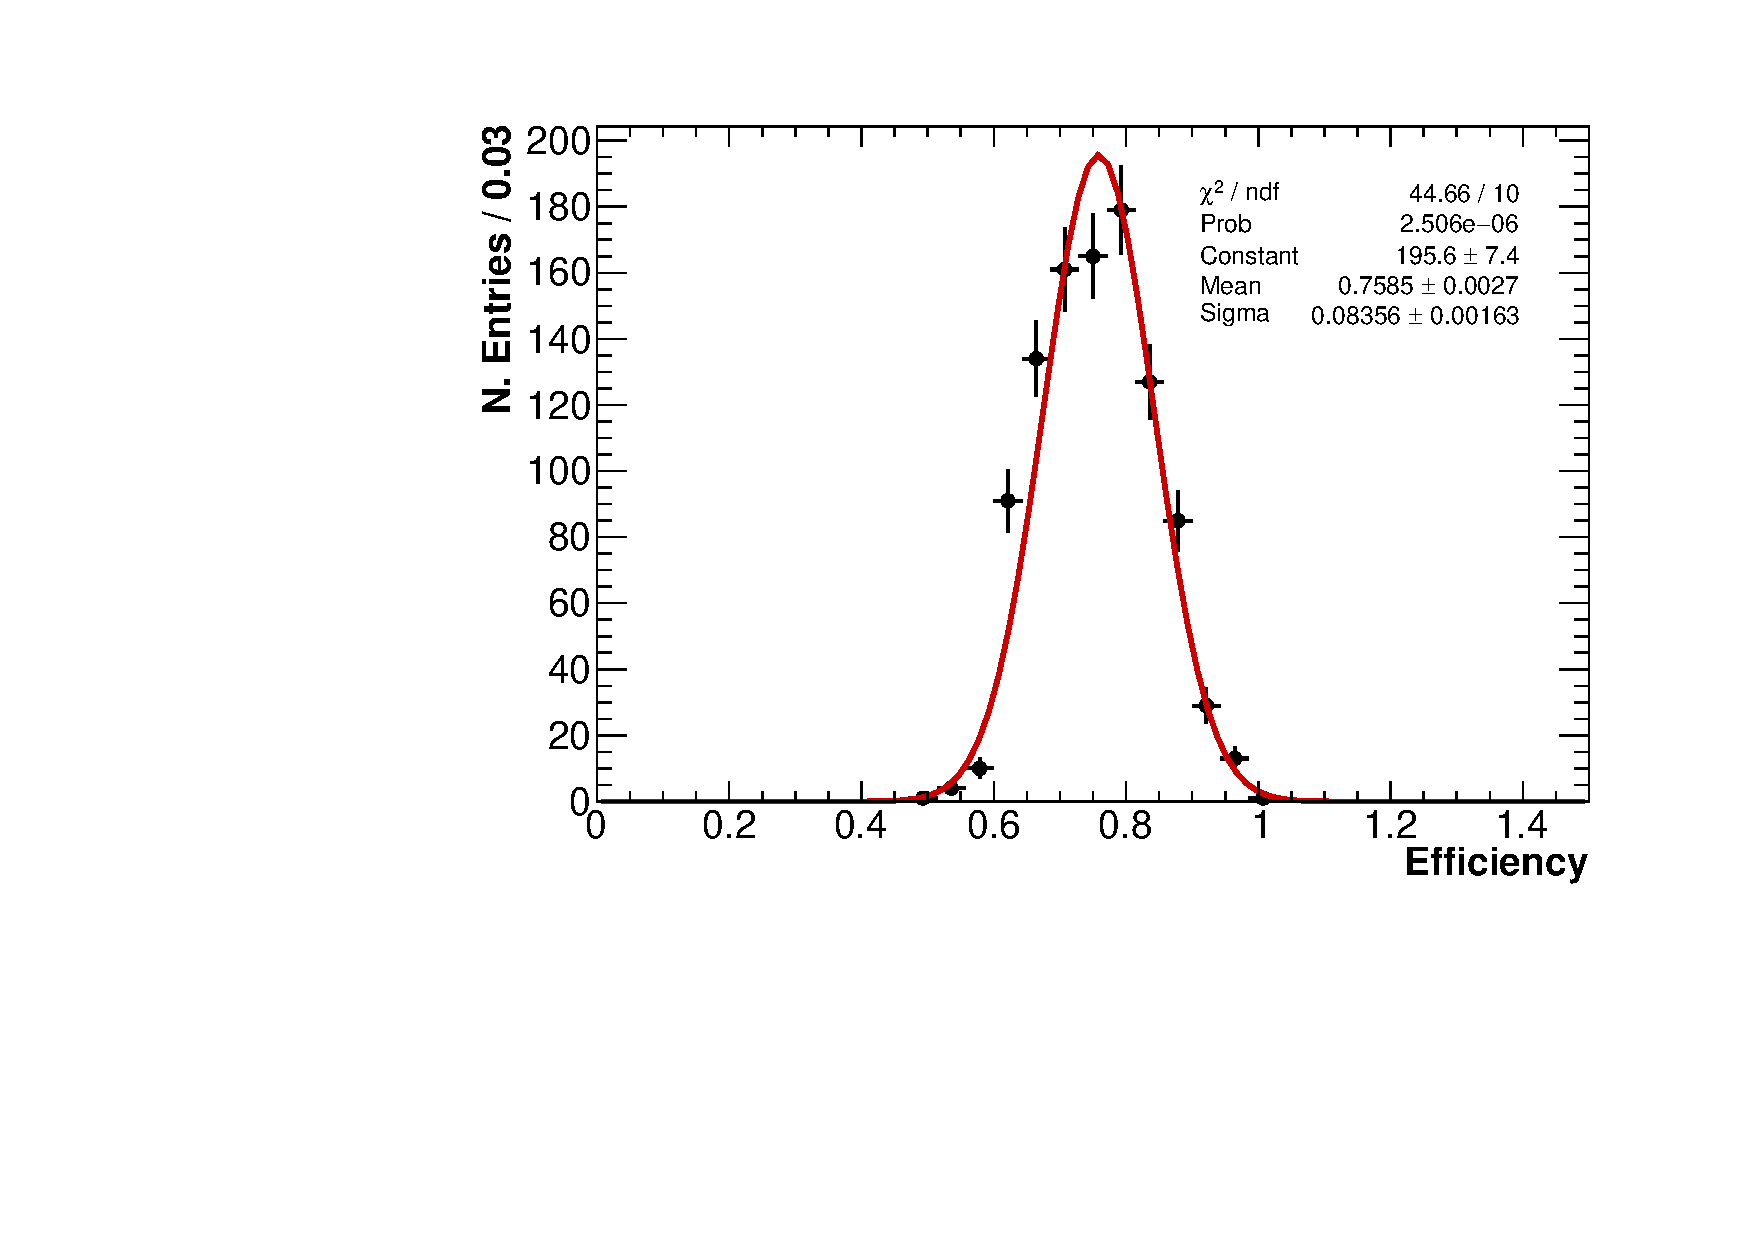
\includegraphics[width=0.7\linewidth]{figures/sampling.pdf}
    \caption{Distribution of the reconstruction efficiency obtained generating 1000 thousand pseudo-experiments with 19 MuCS-triggered events each.} \label{fig:sampling}
  \end{center}
\end{figure}

Thus, low-energy cosmic rays scatter more than high-energy ones and they have a higher probability to be further than $d_{\mathrm{max}}$ from the extrapolated starting point of the MuCS cosmic ray. In the bins where the data reconstruction efficiency has been measured with low statistics, then, it can happen to have MuCS cosmic rays distributed in a small region of the energy spectrum, biasing the measurement of the reconstruction efficiency.

In order to verify if this sampling introduces a systematic effect, we choose the bin with the lowest number of MuCS events, which is 19. We then performed a Monte Carlo simulation, generating one thousand pseudo-experiments with 19 MuCS events sampled from the CORSIKA cosmic-ray energy spectrum with the same starting angles and length of our chosen bin. We filled a histogram with the value of the reconstruction efficiency for each pseudo-experiment and fitted the distribution with a Gaussian (figure \ref{fig:sampling}). The $\sigma$ of the fit is $0.084$, compatible with the statistical error of the same bin which is $0.083$. Thus, we conclude that the energy sampling of the cosmic rays does not introduce a systematic effect.

\subsection{Data/Monte Carlo comparison}
Having included the correction given by the stopped or captured muons and the systematic uncertainty related to the detector non-uniformities, it is possible to compare the data and Monte Carlo reconstruction efficiencies. The three-dimensional efficiency plots shown in figure \ref{fig:3d} can be projected on the bi-dimensional planes ($\theta,\phi$), ($\theta,L$), ($\phi,L$), shown in figure \ref{fig:2d} and on the single axis $\theta$, $\phi$, $L$, shown in figure \ref{fig:1d}.

\begin{figure}[htbp]
  \begin{center}
    \begin{subfigure}{0.6\textwidth}
      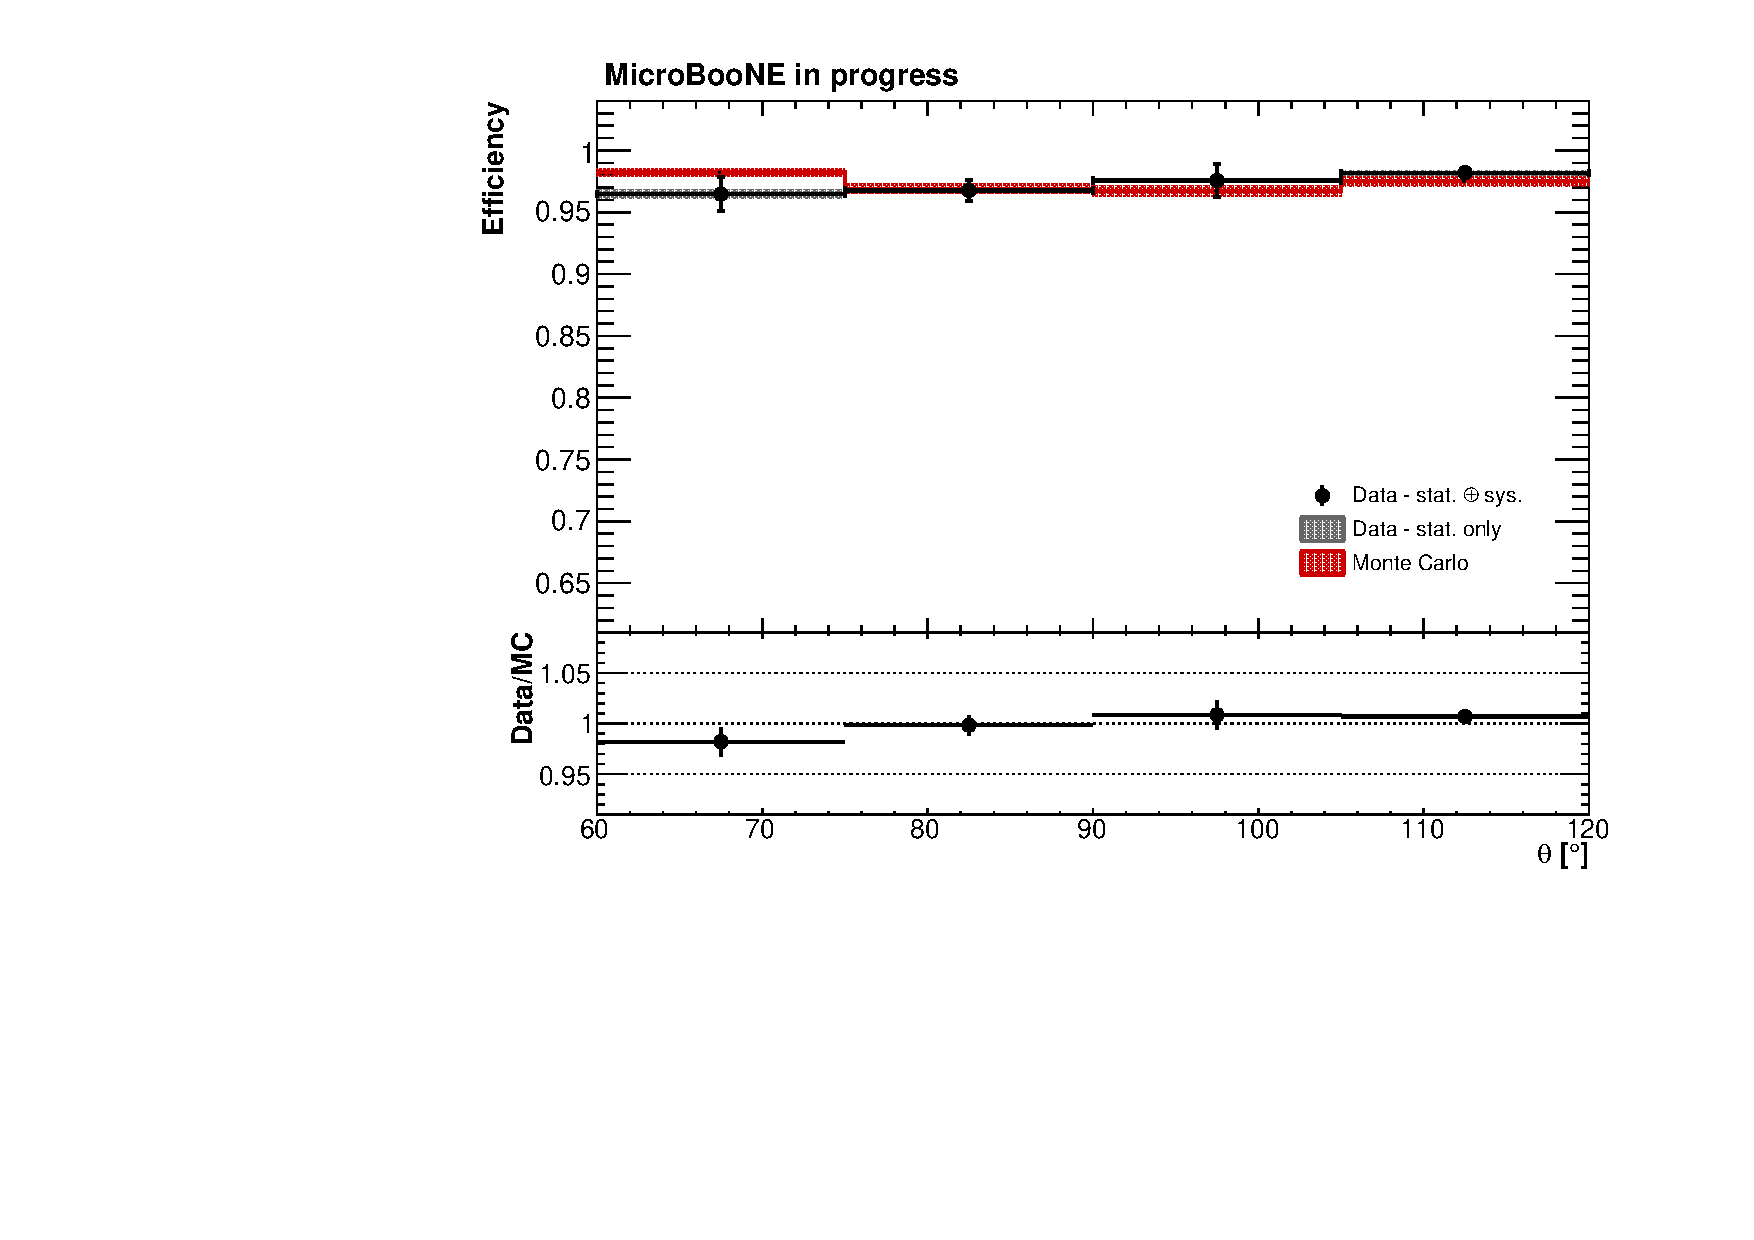
\includegraphics[width=\linewidth]{figures/theta.pdf}
      \caption{$\theta$} \label{fig:theta}
    \end{subfigure}
    \begin{subfigure}{0.6\textwidth}
      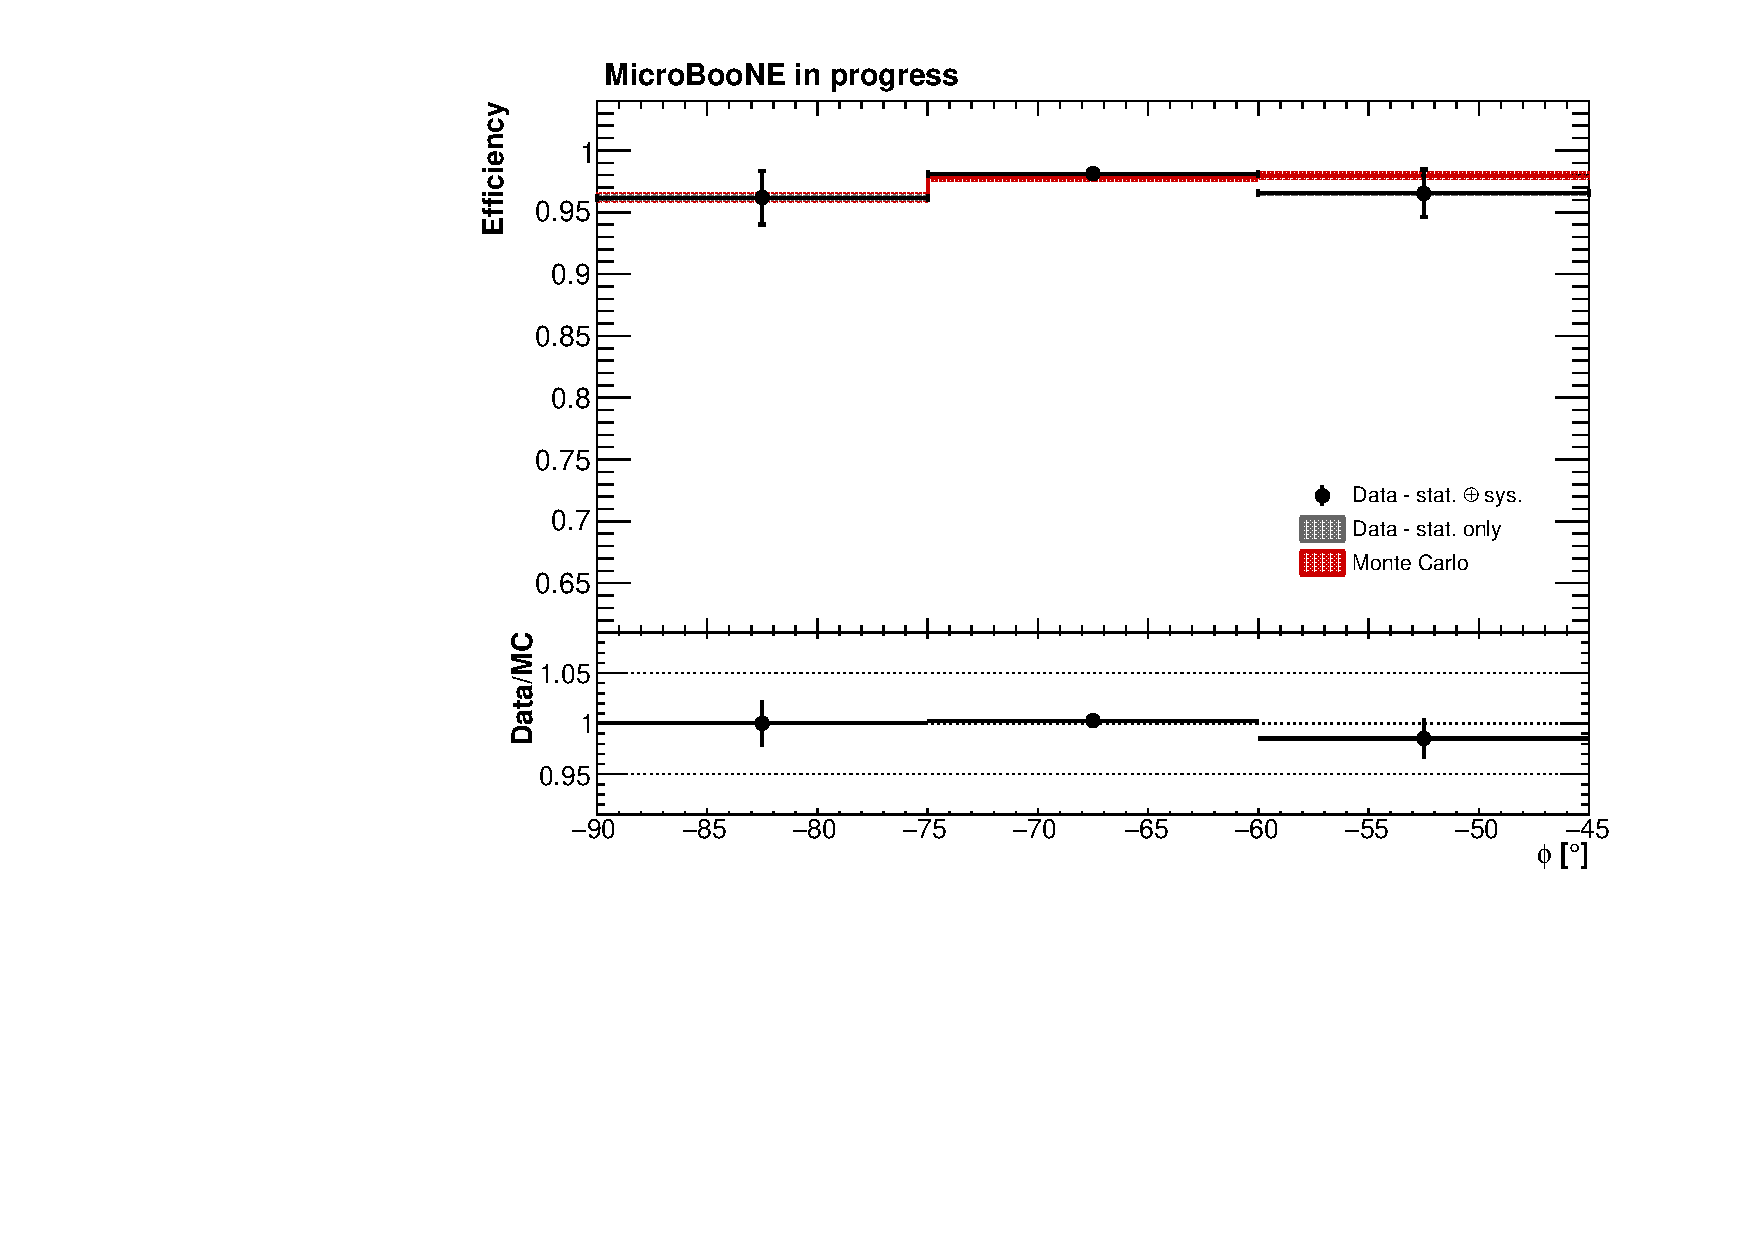
\includegraphics[width=\linewidth]{figures/phi.pdf}
      \caption{$\phi$} \label{fig:phi}
    \end{subfigure}
    \begin{subfigure}{0.6\textwidth}
      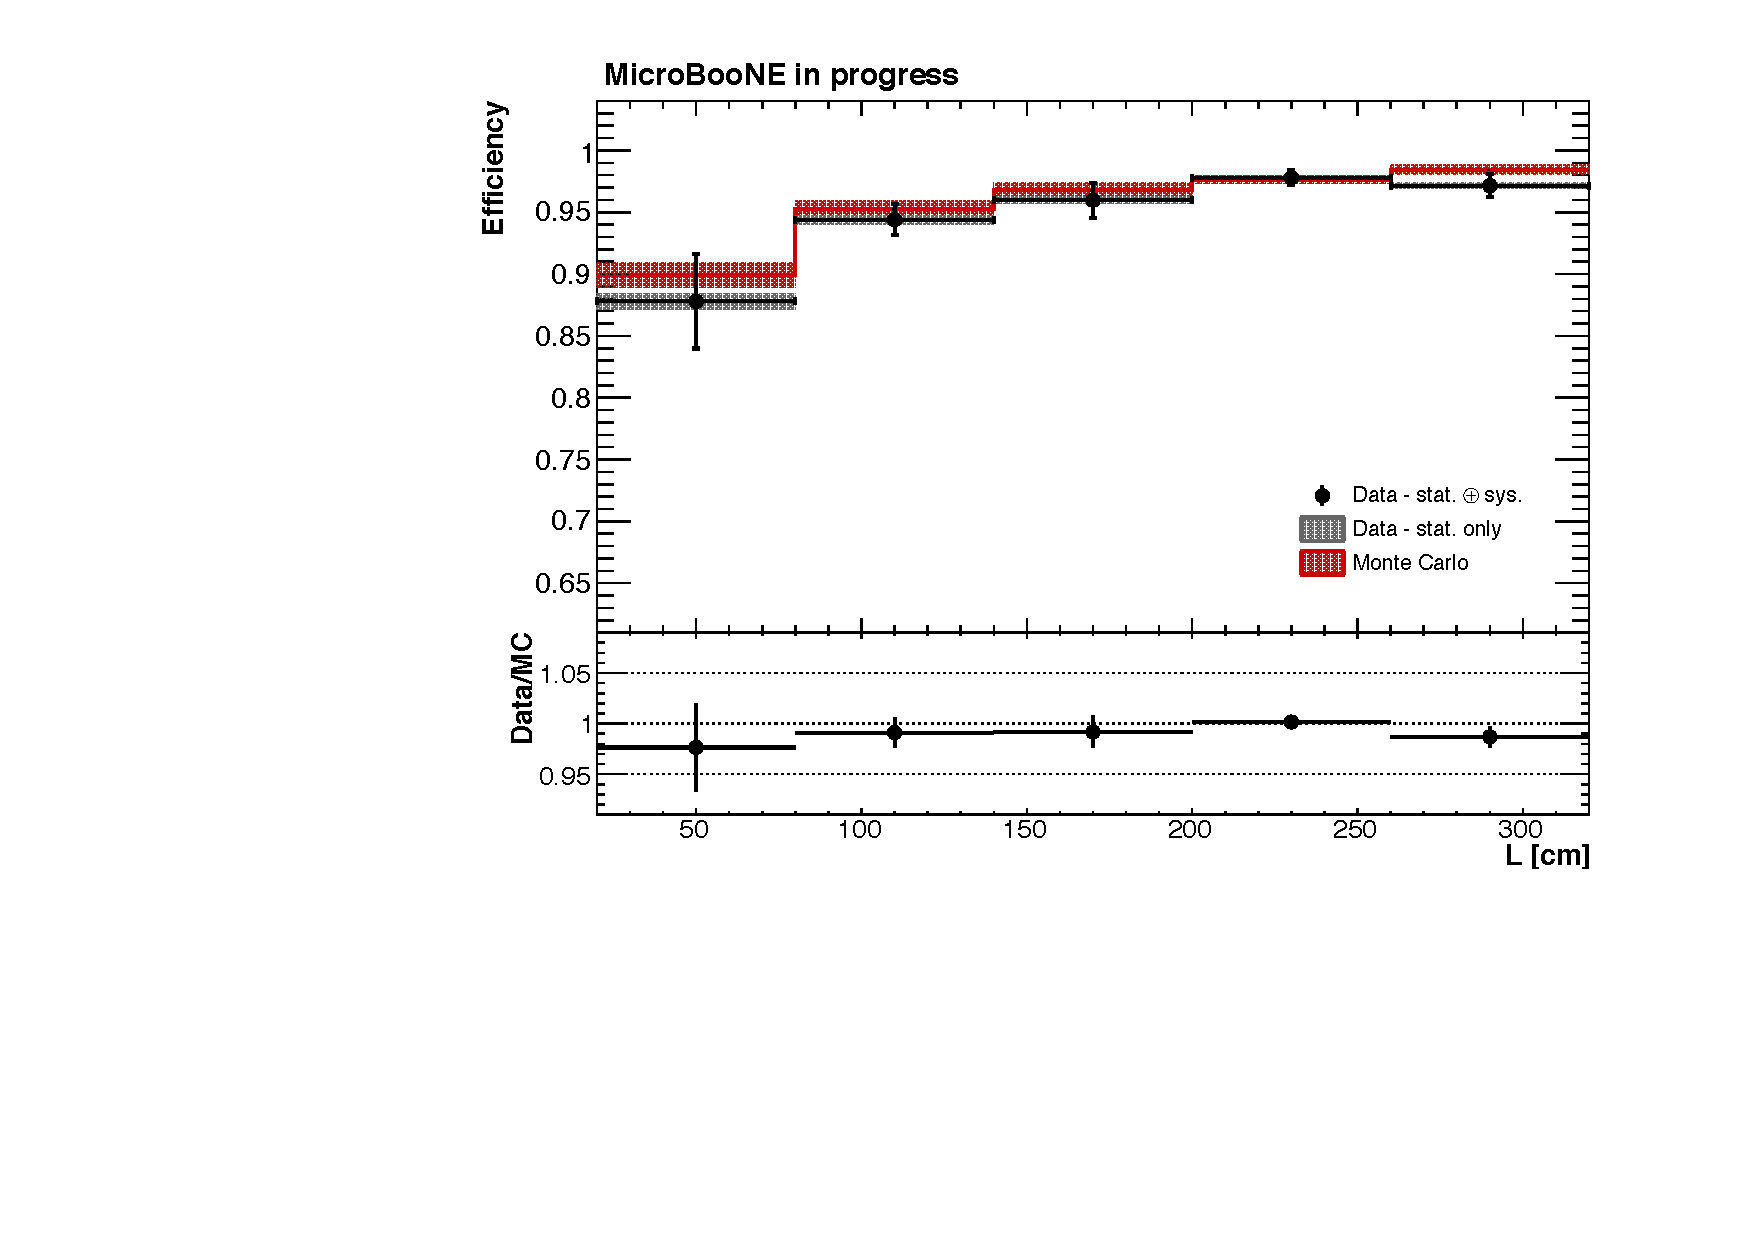
\includegraphics[width=\linewidth]{figures/l.pdf}
      \caption{$L$} \label{fig:l}
    \end{subfigure}
    \caption{Monte Carlo (red line) and data (black points) reconstruction efficiency as a function of the starting angles $\theta$, $\phi$ and the extrapolated track length $L$. Monte Carlo errors are statistical-only.}\label{fig:1d}
  \end{center}
\end{figure}

Taking into account the systematic uncertainties given by (1) the decay-in-flight correction factor (0.1\%, section \ref{sec:dif}), (2) the detector non-uniformities (1.1\%, section \ref{sec:wires}), and (3) the $P/A$ correcting factor (0.2\%, section \ref{sec:reco}), the obtained data/Monte Carlo agreement is satisfactory, with almost every bin with a data/Monte Carlo ratio within 2$\sigma$ of unity. As expected, the reconstruction efficiency is proportional to the expected track length $L$ in the TPC, since longer tracks correspond, in general, to a larger number of hit wires and they are then easier to reconstruct.

The overall reconstruction efficiency, obtained integrating the three-dimensional plot, is:
\begin{align*}
\epsilon_{\mathrm{data}} &= 97.1 \pm 0.1~\mathrm{(stat)} \pm 1.4~\mathrm{(sys)}~\%\\
\epsilon_{\mathrm{MC}} &= 97.3 \pm 0.1~\%
\end{align*} for data and Monte Carlo, respectively. The agreement between the two values is within the error.

\begin{figure}[htbp]
  \begin{subfigure}{0.33\textwidth}
    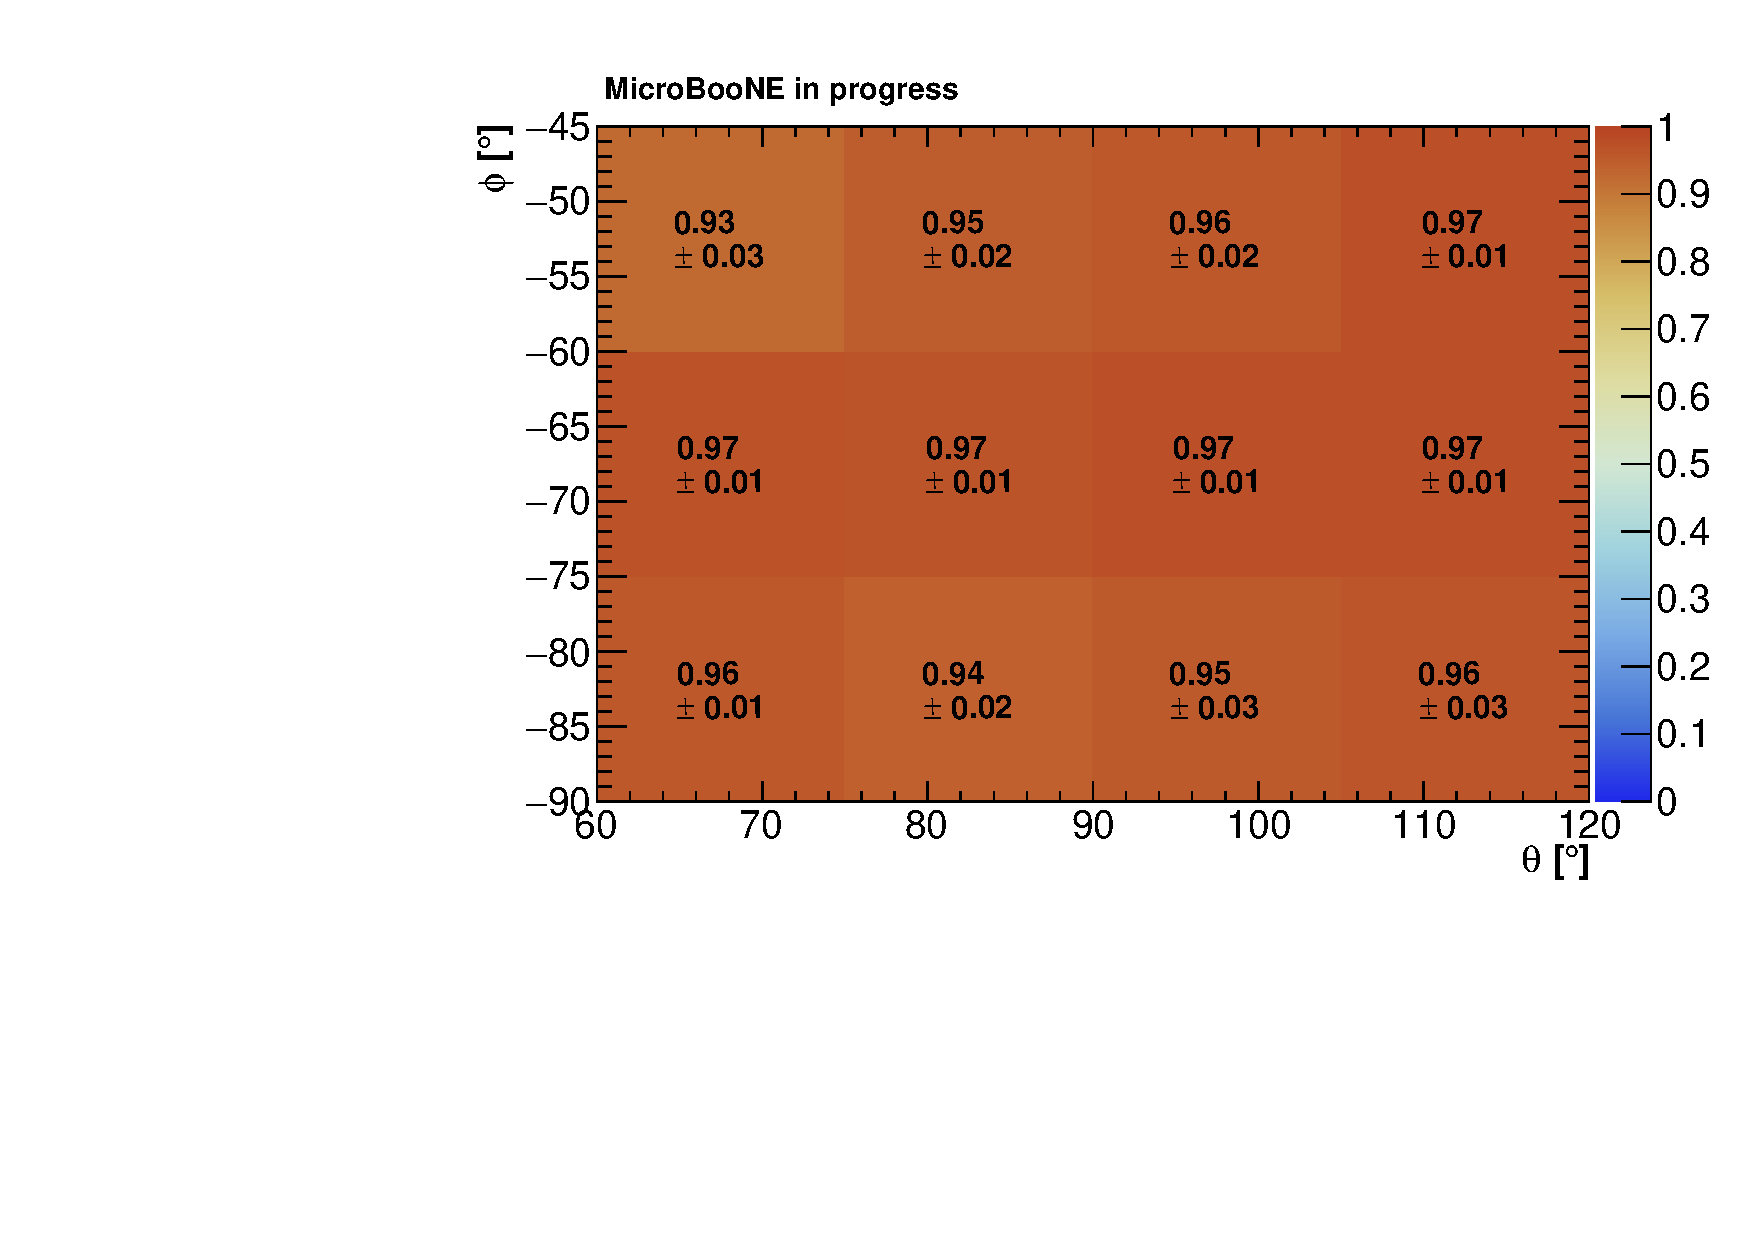
\includegraphics[width=\linewidth]{figures/e_theta_phi.pdf}
    \caption{$(\theta,\phi)$ - Data}
  \end{subfigure}\begin{subfigure}{0.33\textwidth}
  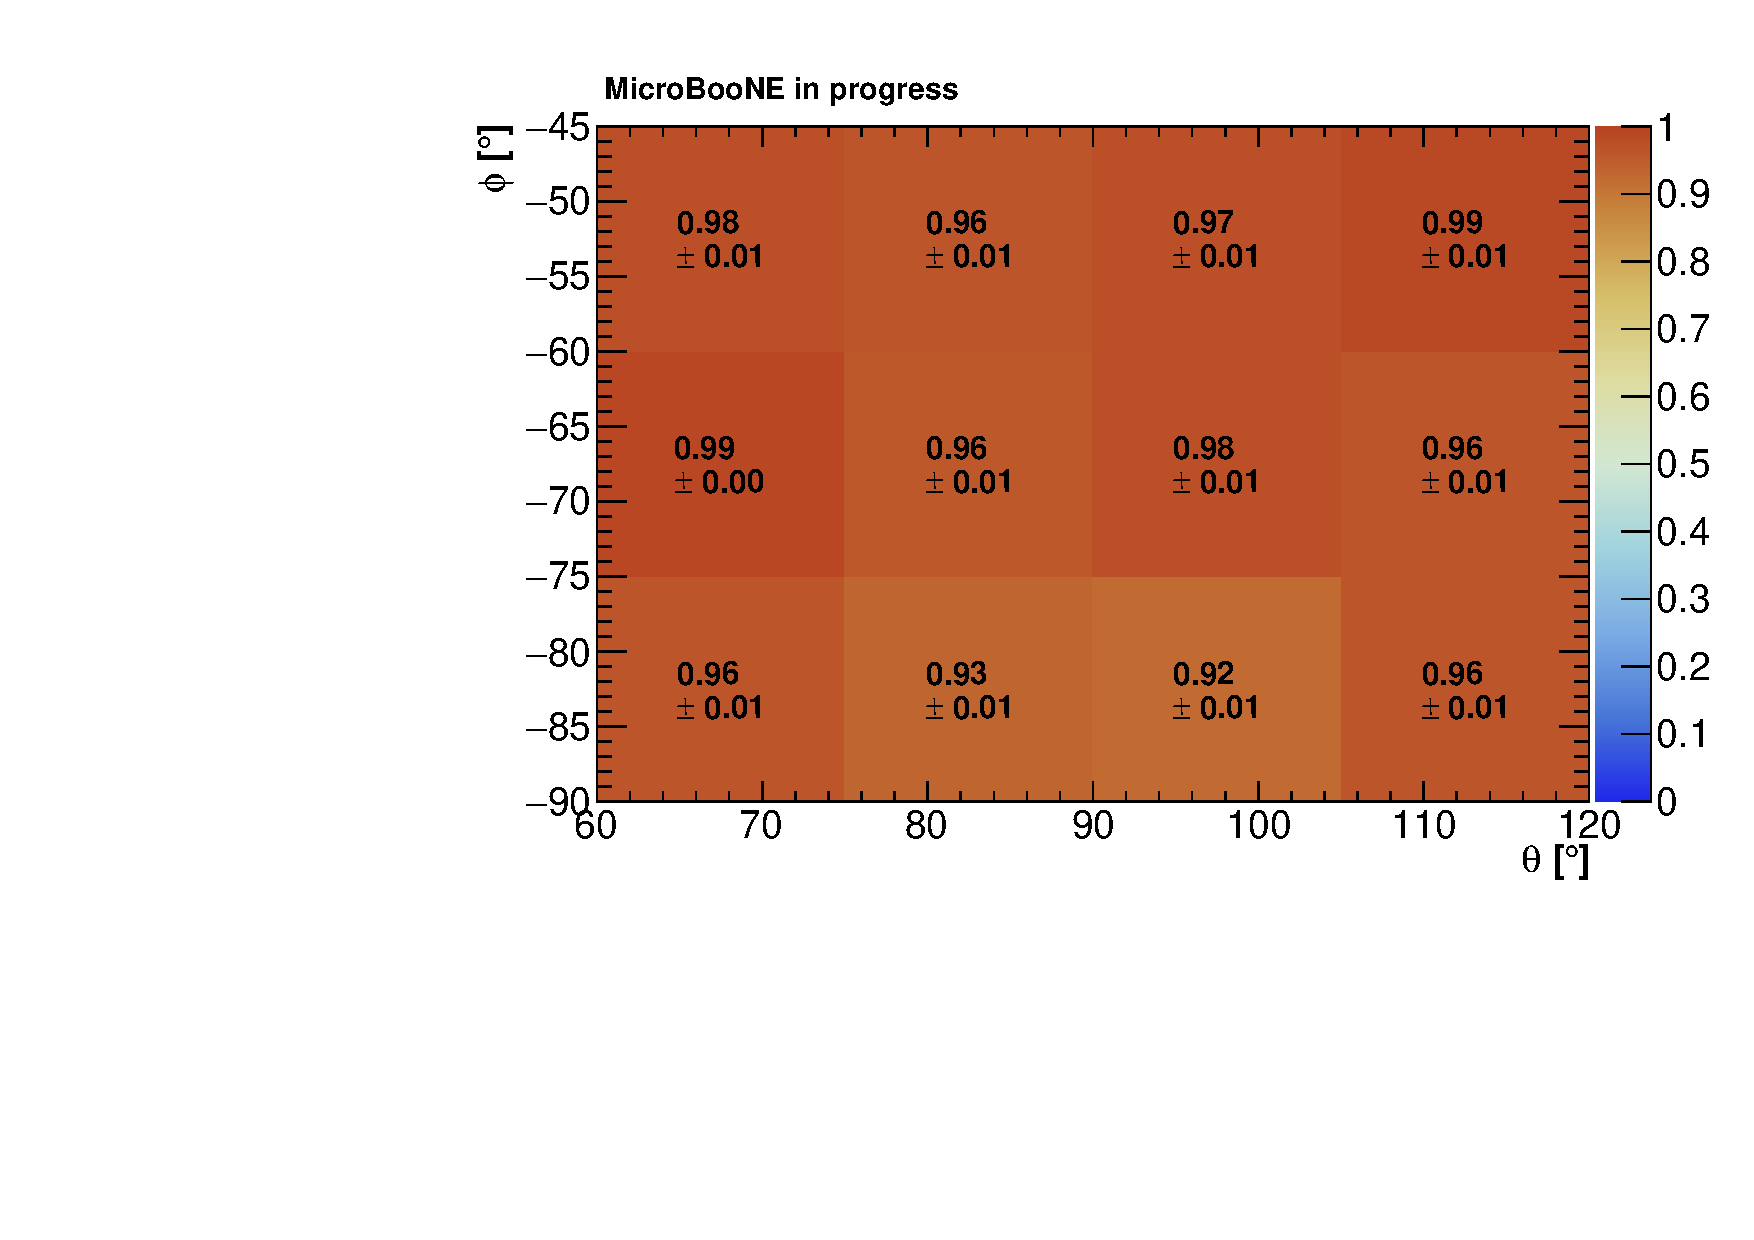
\includegraphics[width=\linewidth]{figures/theta_phi_mc.pdf}
  \caption{$(\theta,\phi)$ - Monte Carlo}
  \end{subfigure}\begin{subfigure}{0.33\textwidth}
  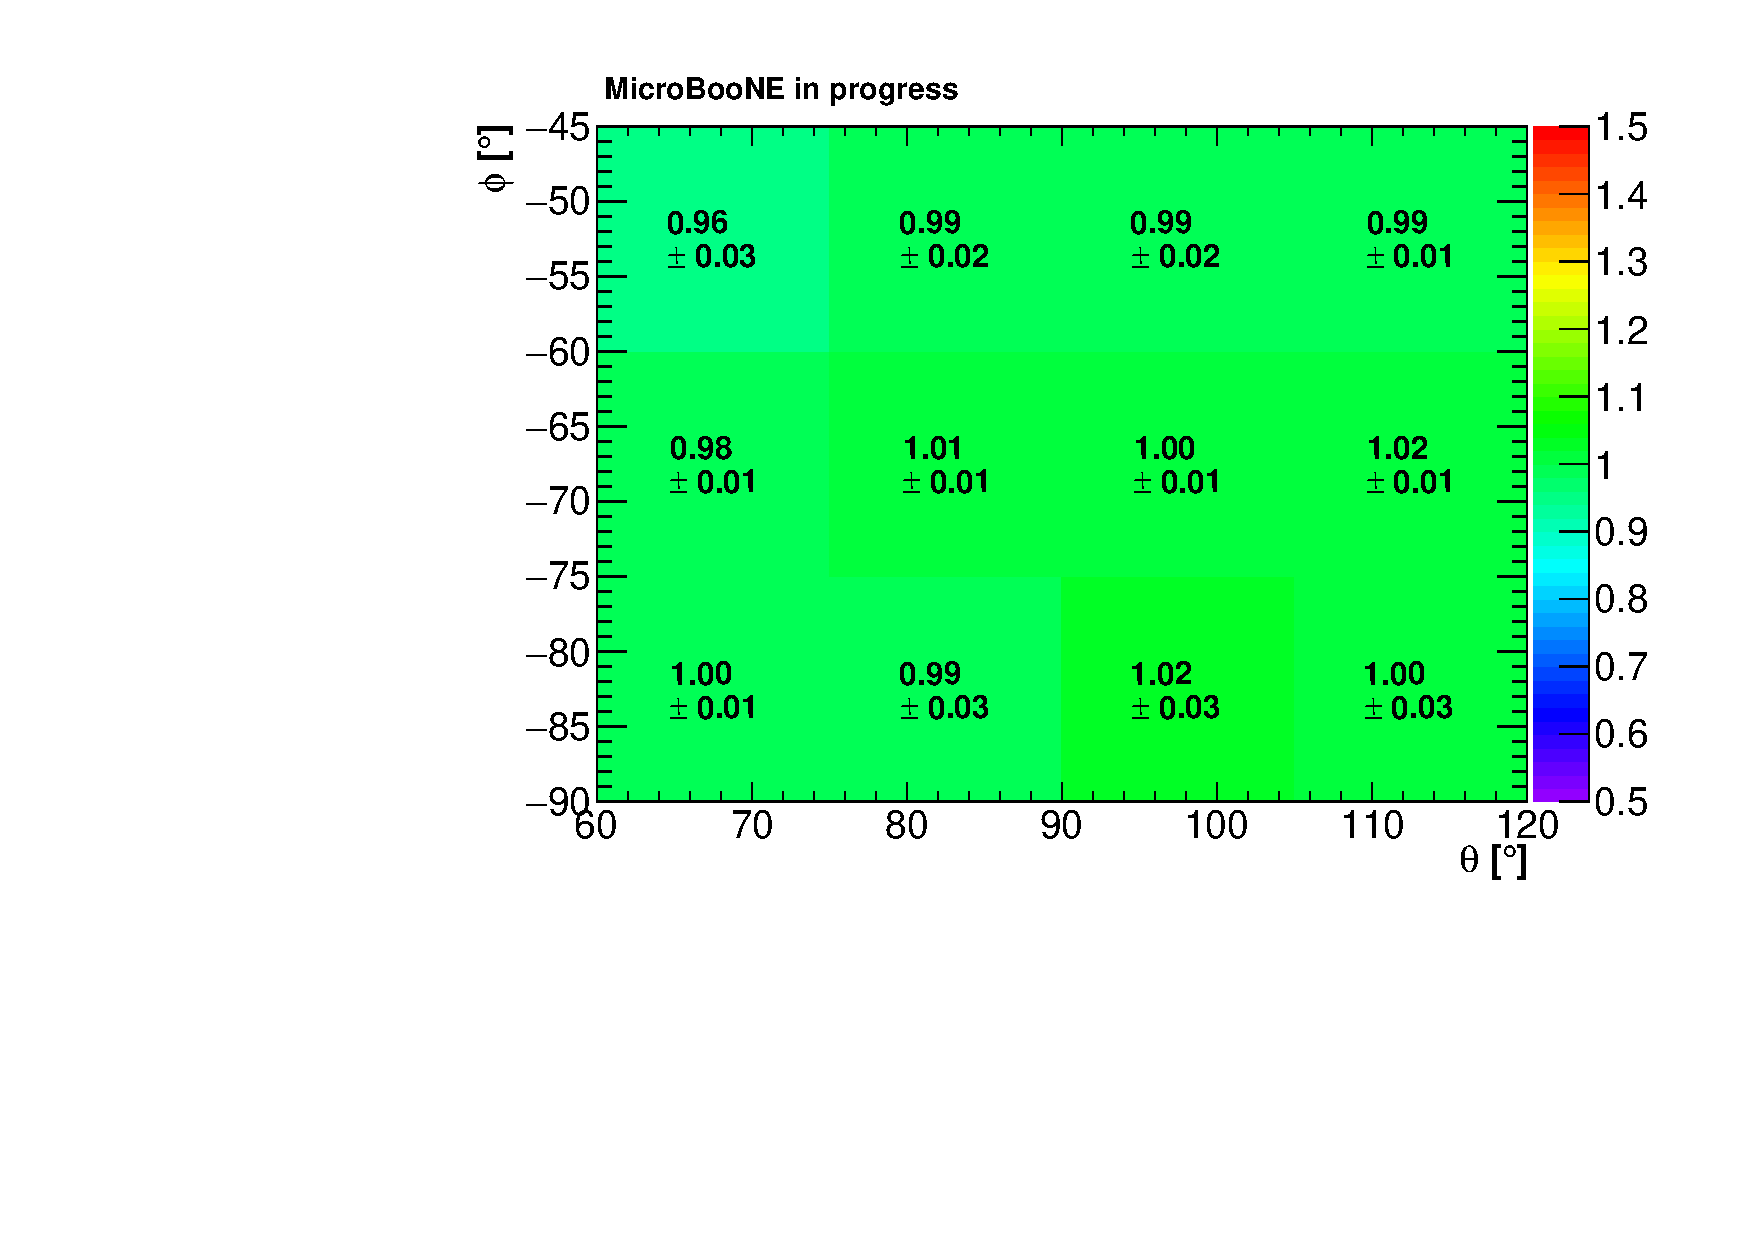
\includegraphics[width=\linewidth]{figures/theta_phi.pdf}
  \caption{$(\theta,\phi)$ - Data/Monte Carlo}
\end{subfigure}
\begin{subfigure}{0.33\textwidth}
  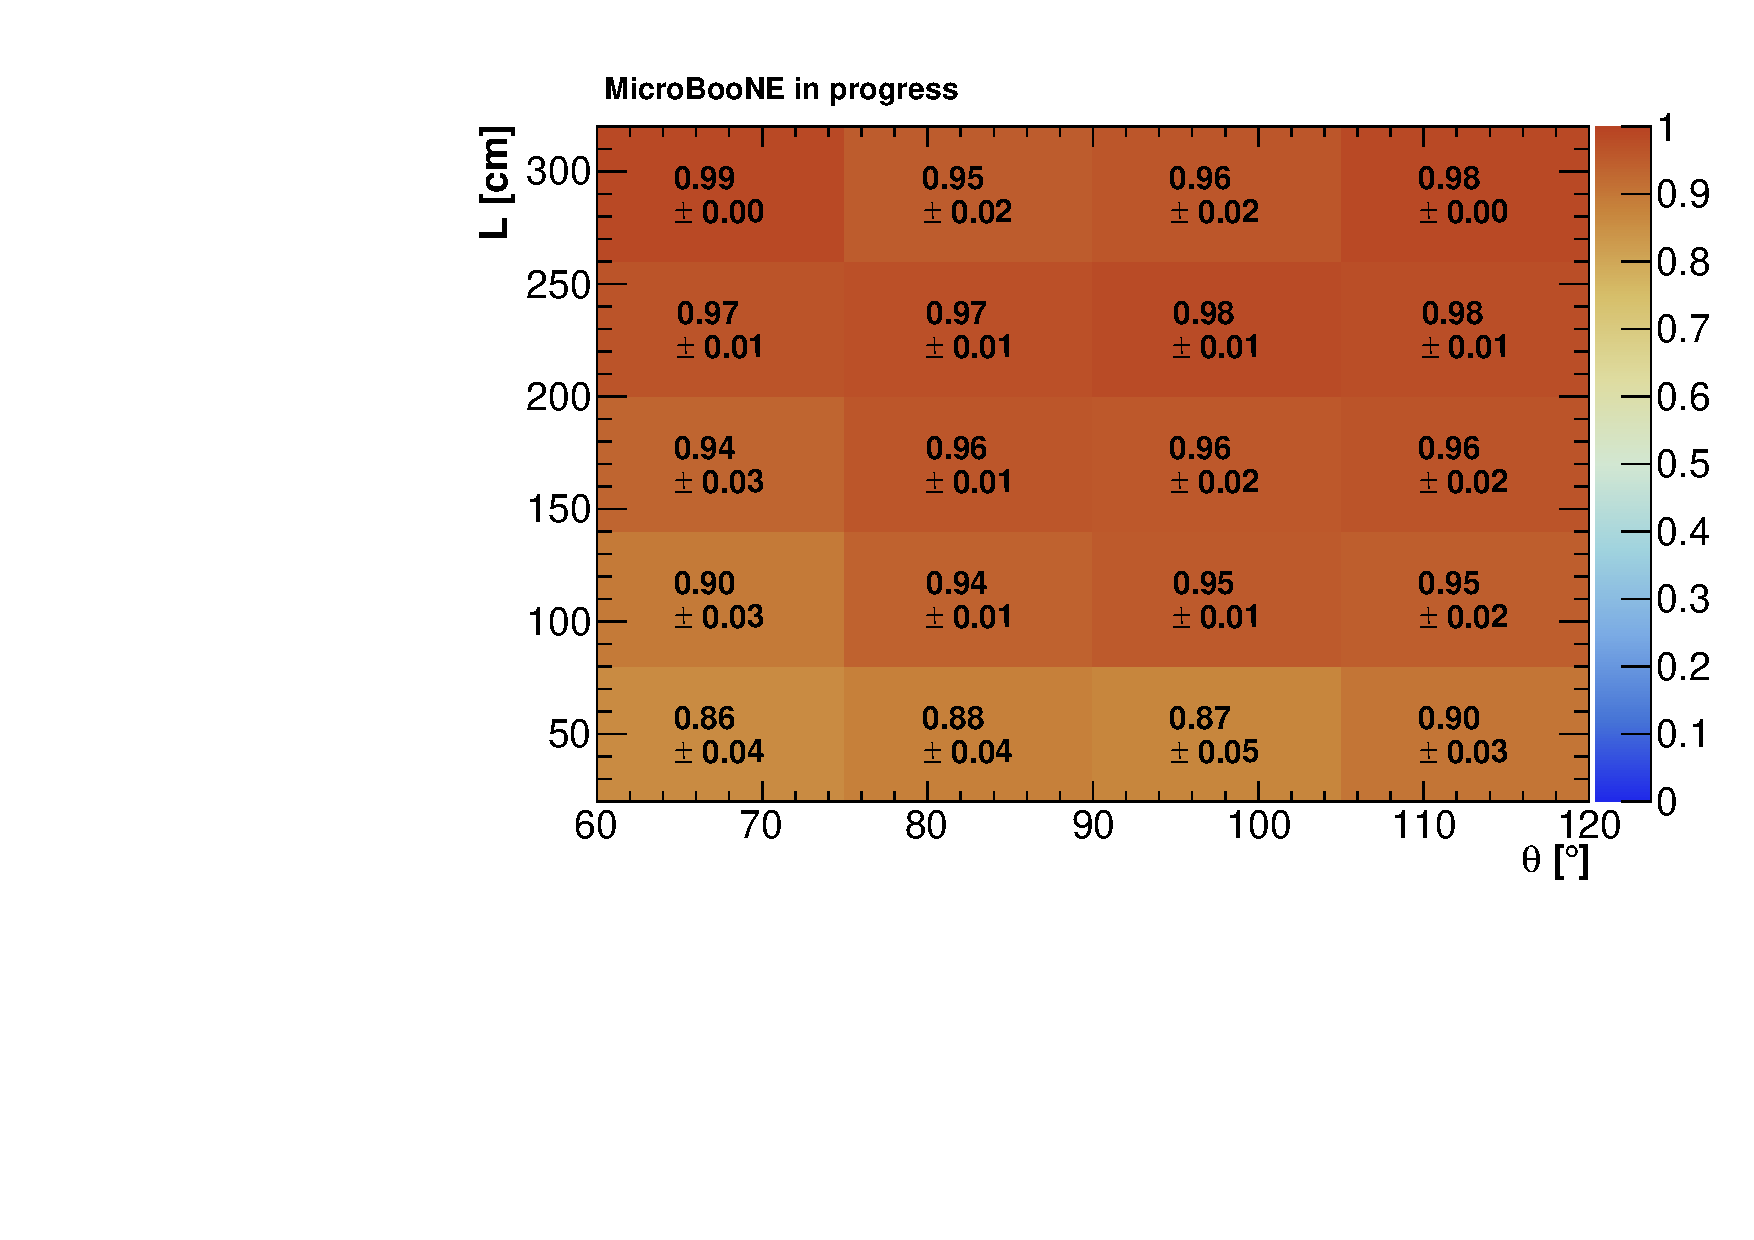
\includegraphics[width=\linewidth]{figures/e_theta_l.pdf}
  \caption{$(\theta,L)$ - Data}
\end{subfigure}\begin{subfigure}{0.33\textwidth}
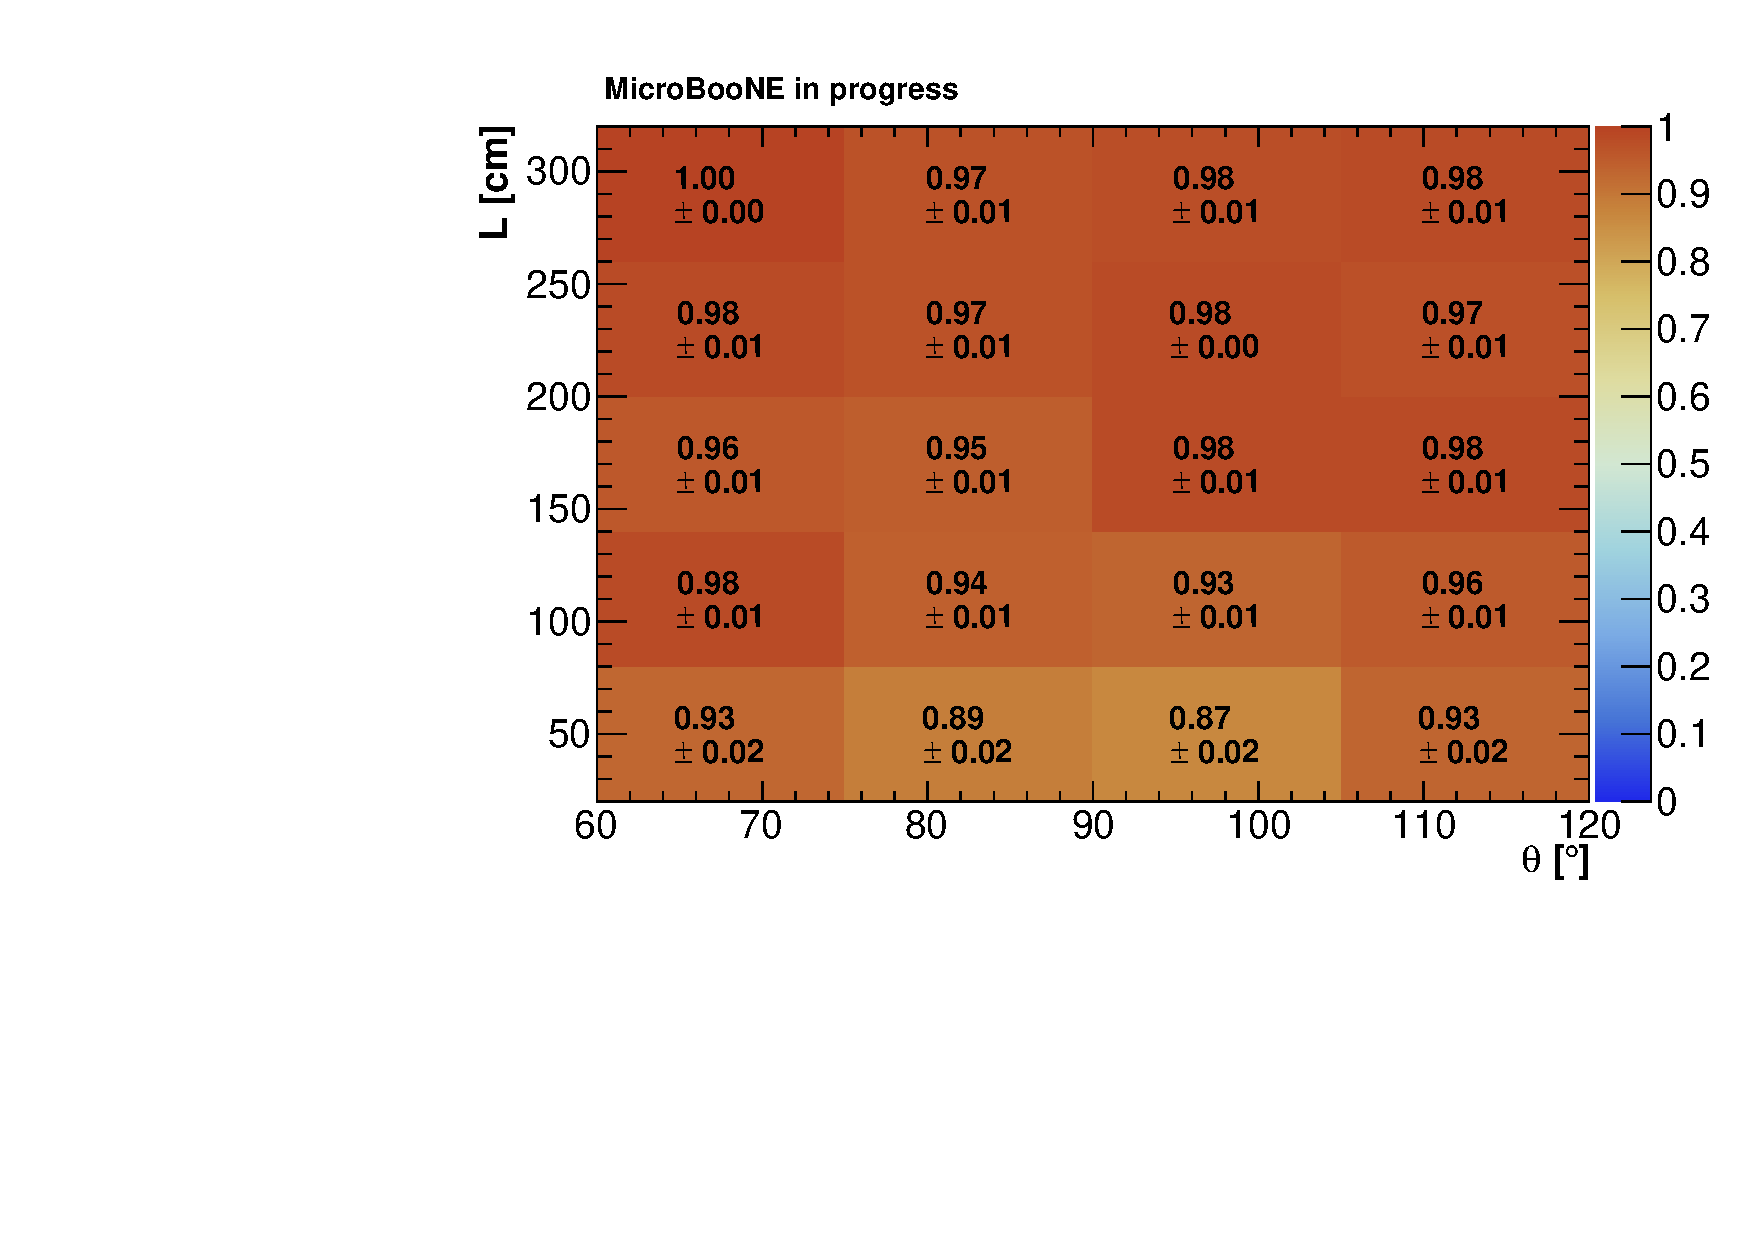
\includegraphics[width=\linewidth]{figures/theta_l_mc.pdf}
\caption{$(\theta,L)$ - Monte Carlo}
\end{subfigure}\begin{subfigure}{0.33\textwidth}
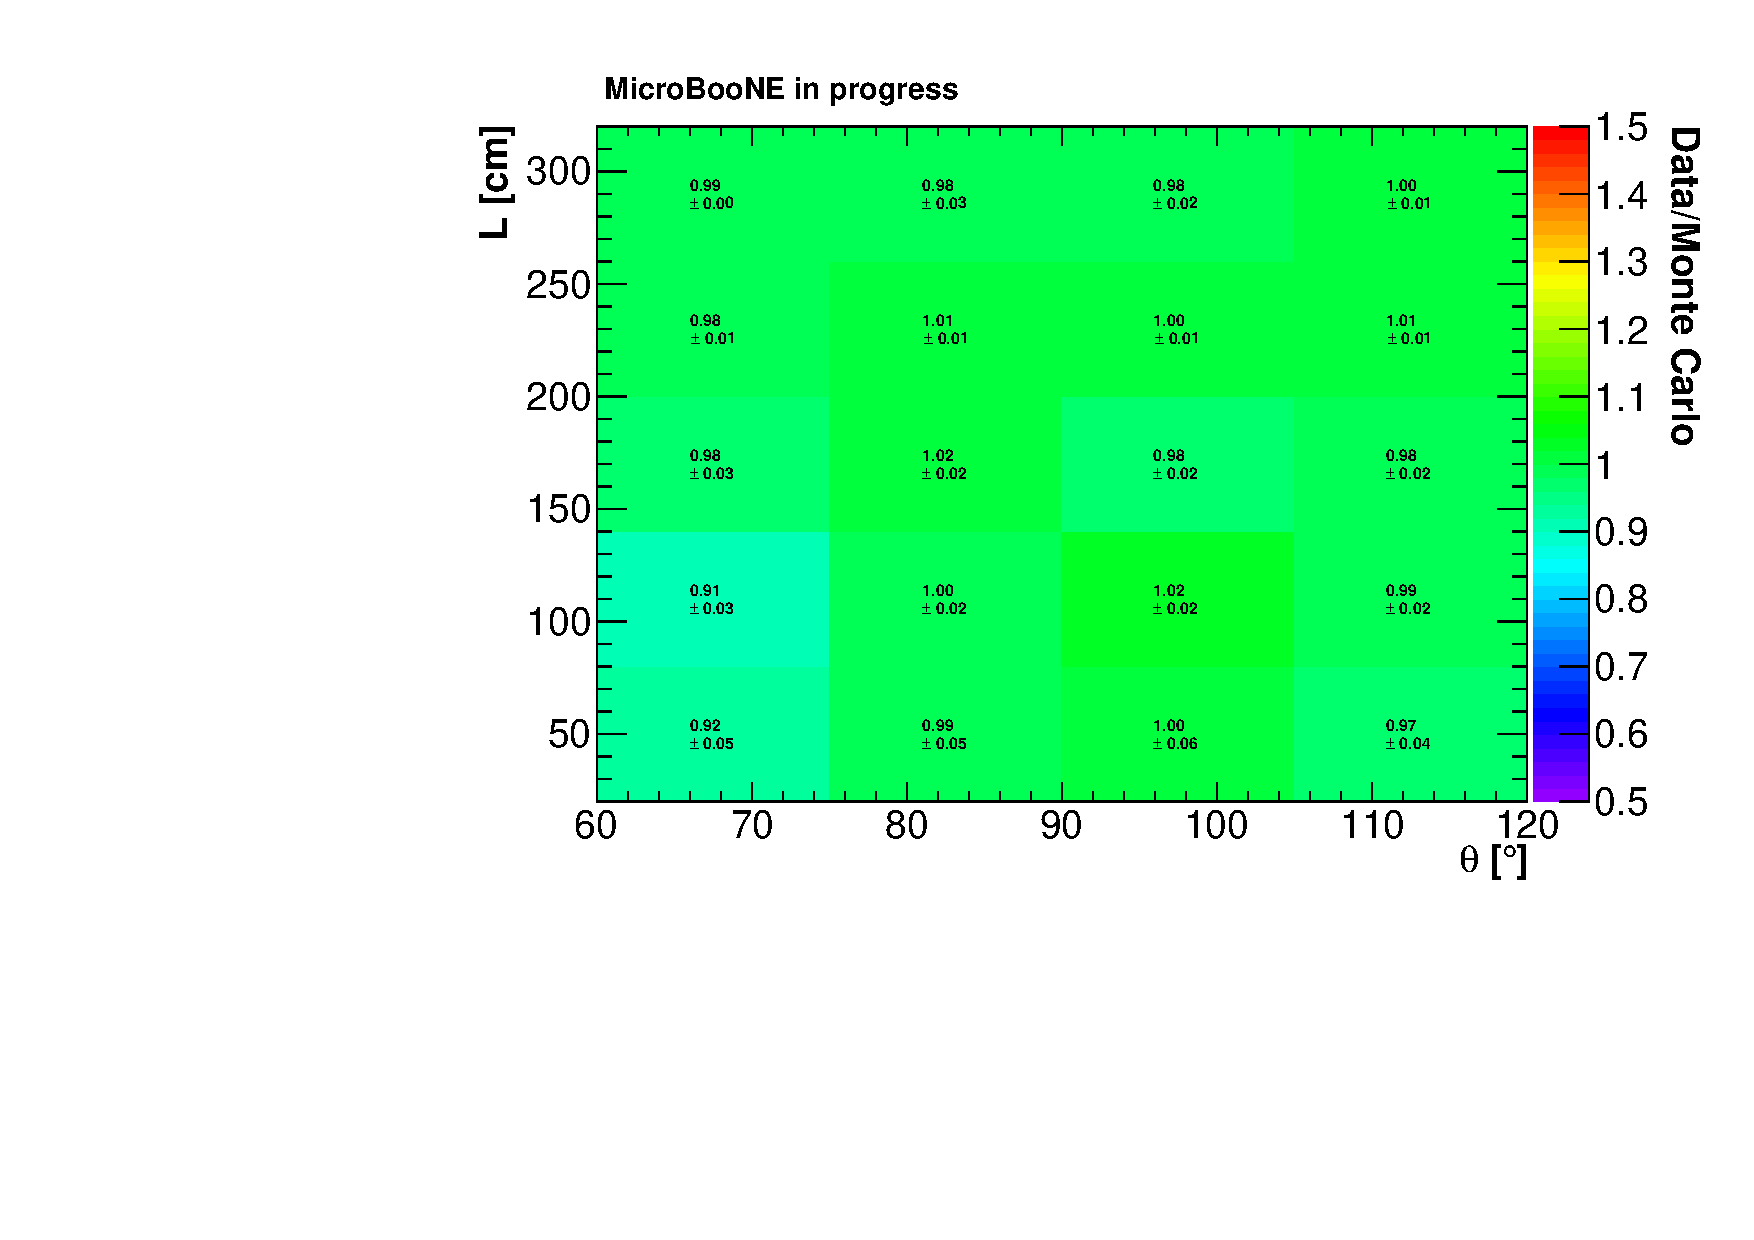
\includegraphics[width=\linewidth]{figures/theta_l.pdf}
\caption{$(\theta,L)$ - Data/Monte Carlo}
\end{subfigure}
\begin{subfigure}{0.33\textwidth}
  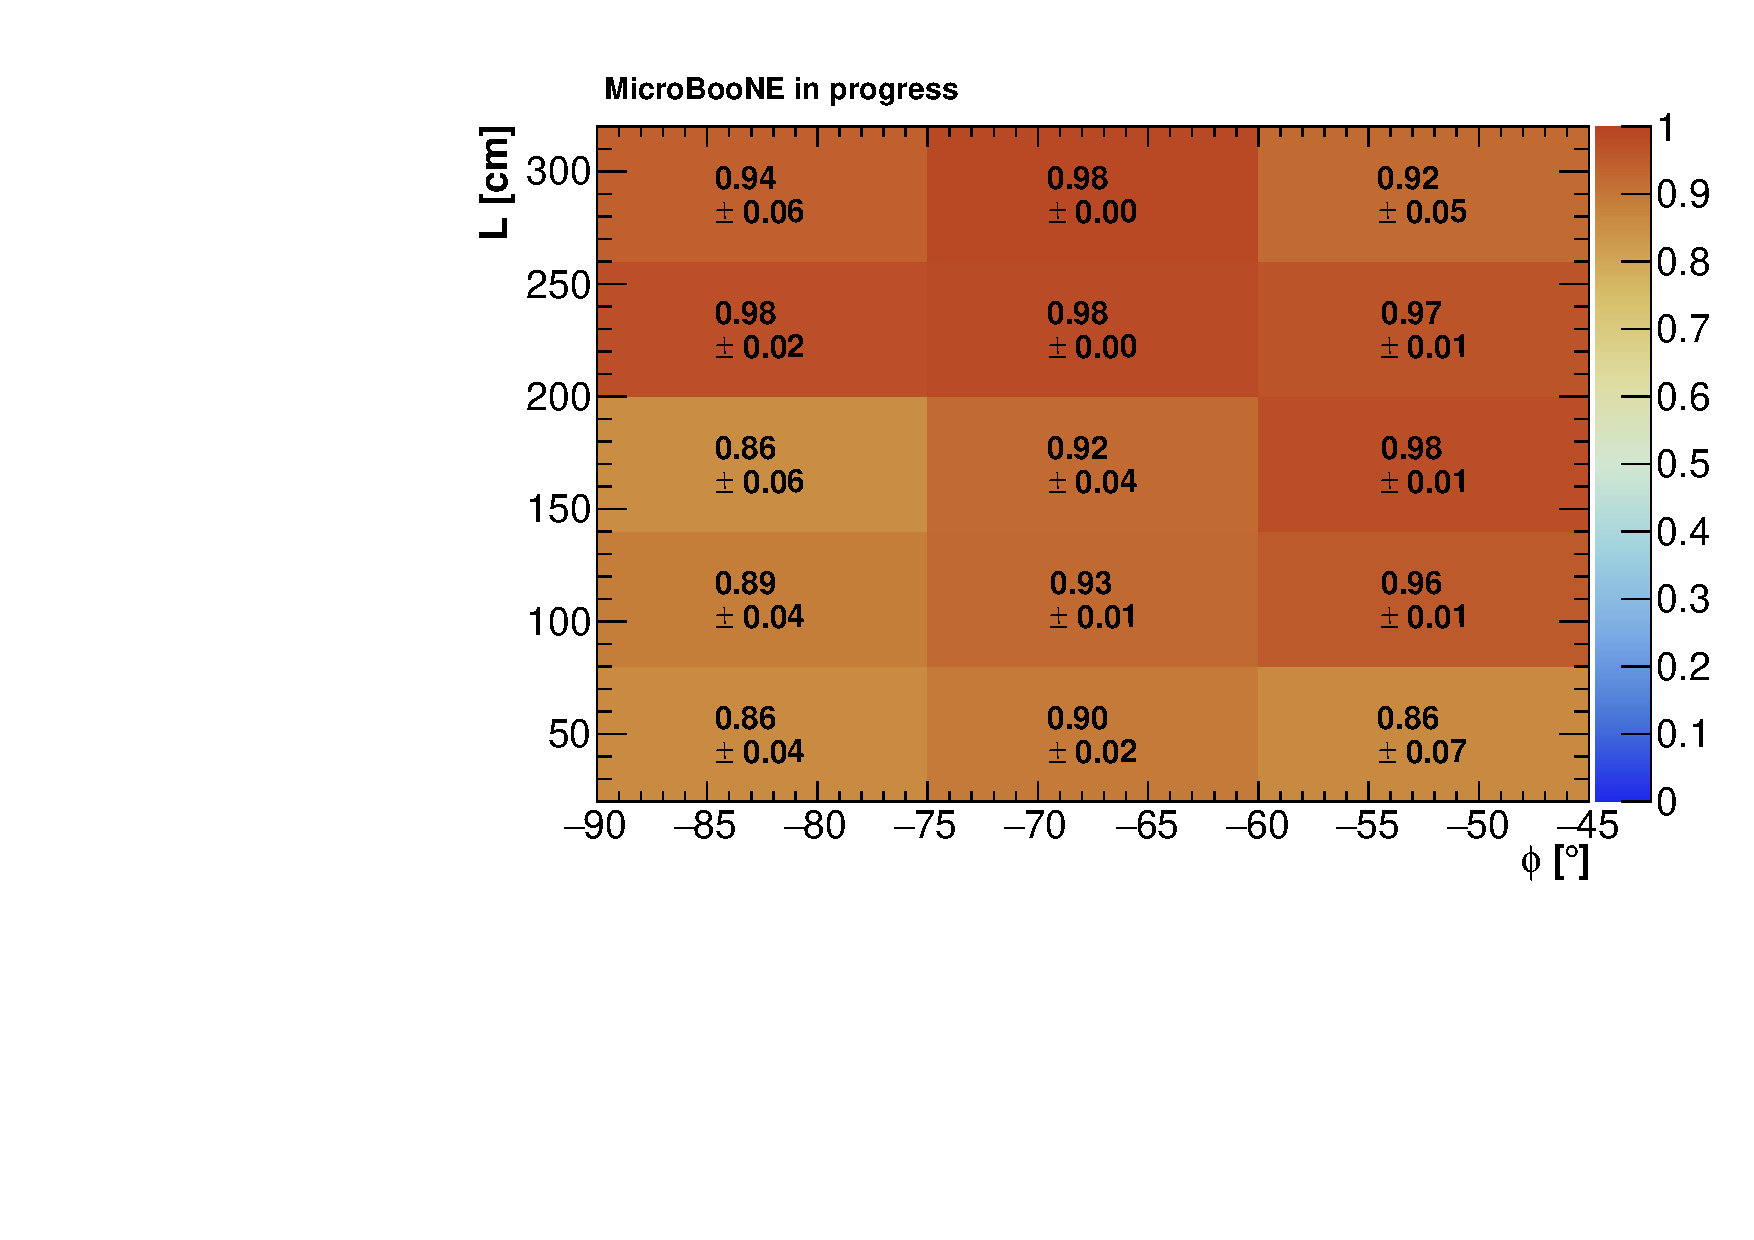
\includegraphics[width=\linewidth]{figures/e_phi_l.pdf}
  \caption{$(\phi,L)$ - Data}
\end{subfigure}\begin{subfigure}{0.33\textwidth}
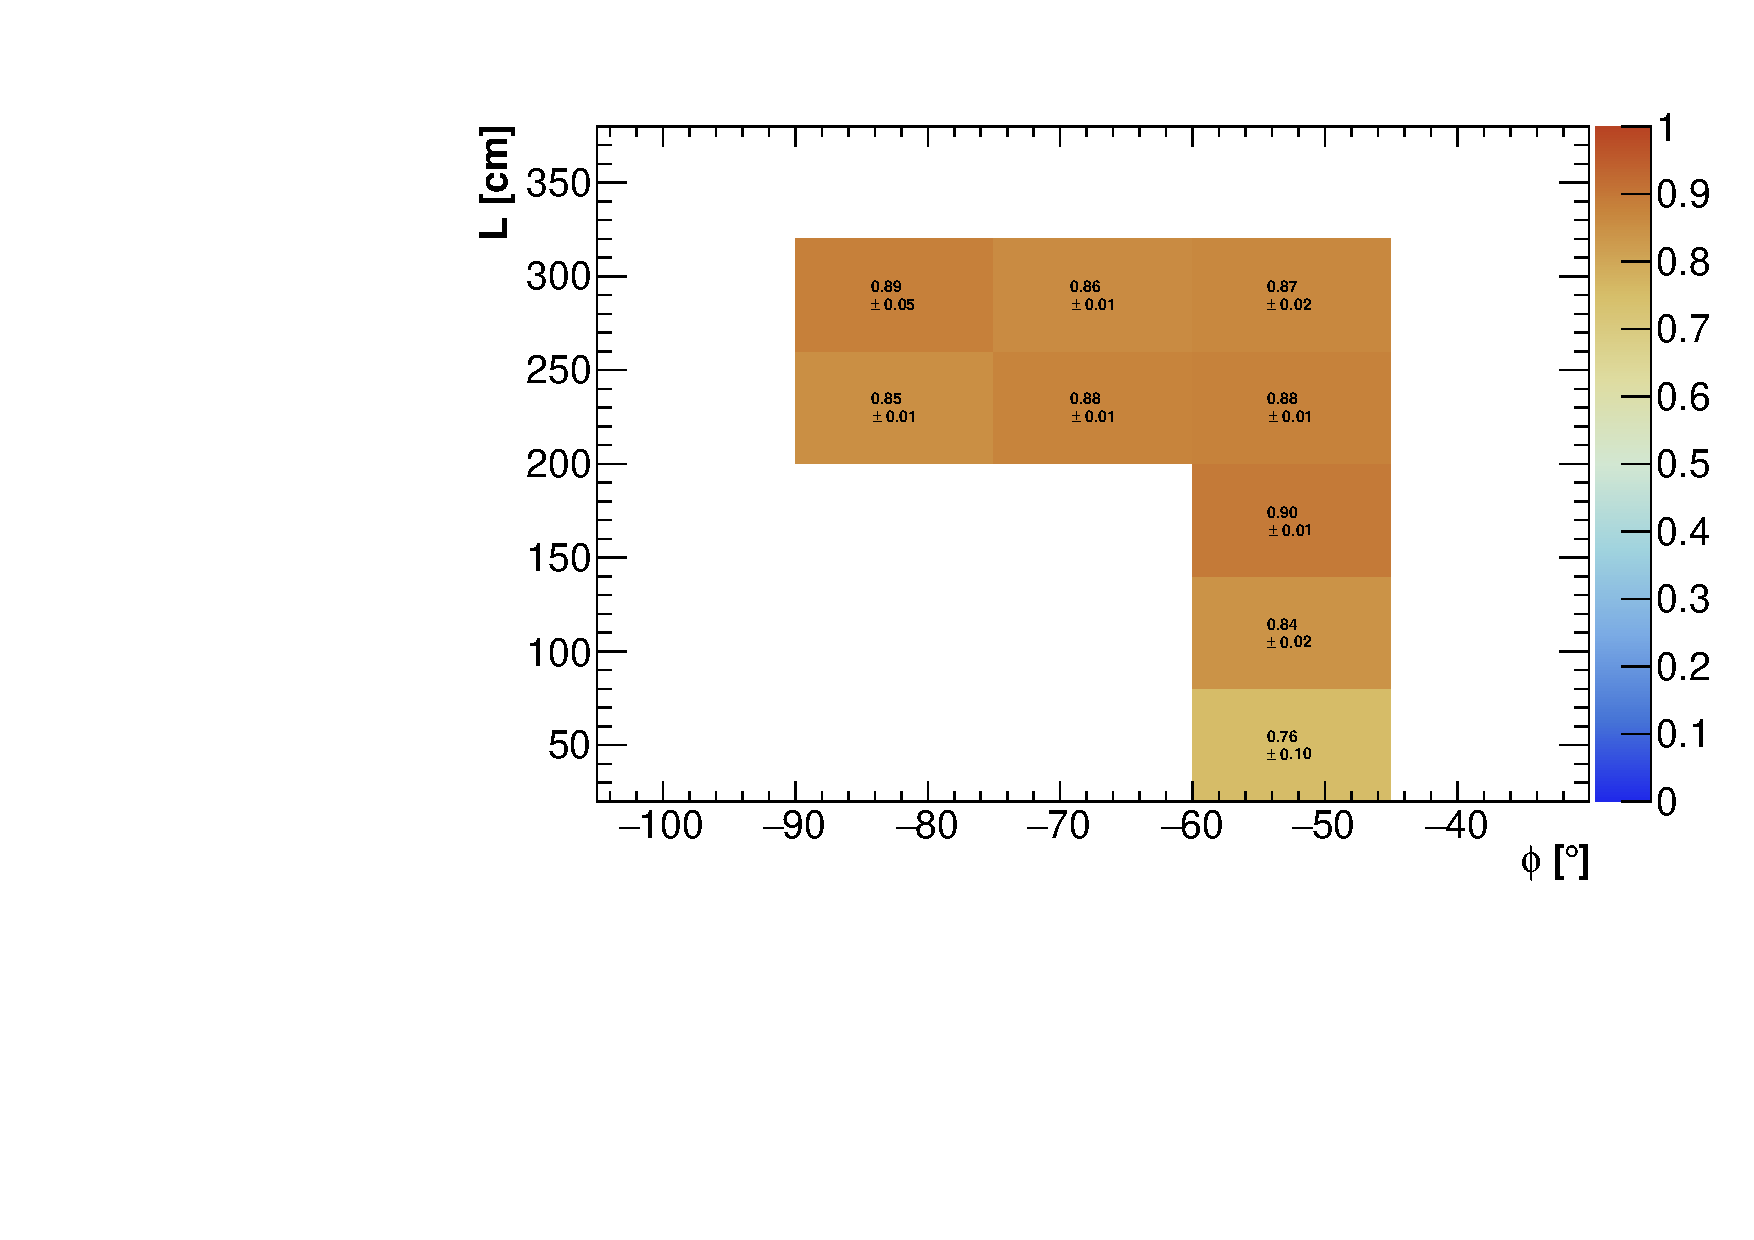
\includegraphics[width=\linewidth]{figures/phi_l_mc.pdf}
\caption{$(\phi,L)$ - Monte Carlo}
\end{subfigure}\begin{subfigure}{0.33\textwidth}
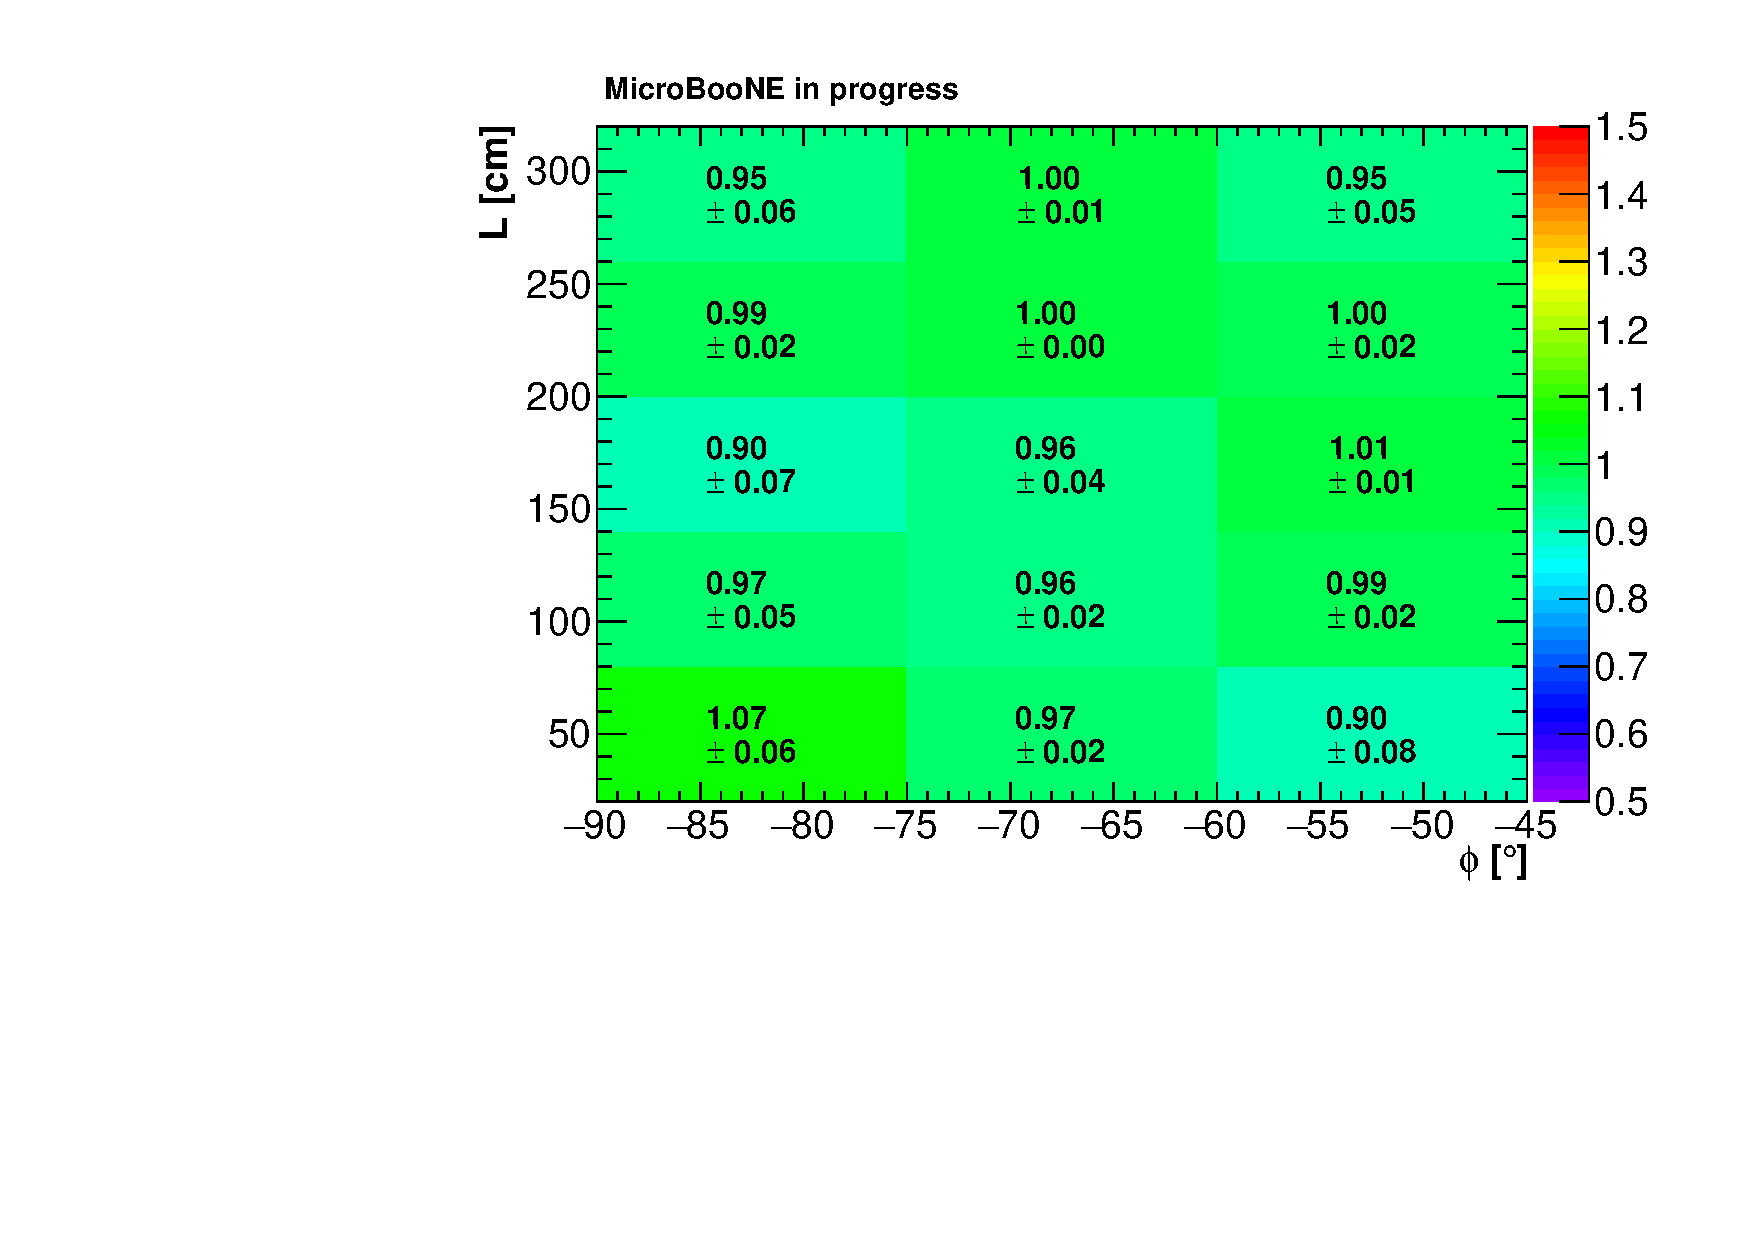
\includegraphics[width=\linewidth]{figures/phi_l.pdf}
\caption{$(\phi,L)$ - Data/Monte Carlo}
\end{subfigure}
\caption{Two-dimensional reconstruction efficiencies for data (left), Monte Carlo (center) and their ratio (right). Data errors include systematic effects. Monte Carlo errors are statistical-only.}\label{fig:2d}
\end{figure}

\section{Summary and plans}
This analysis showed that it is possible to match hits in a muon counter system to a track in the LArTPC and that by comparing the number of events triggered by the MuCS with the number of events with MuCS-tagged tracks we can measure the data reconstruction efficiency.

This efficiency, obtained with the procedure described in section \ref{sec:reco}, has been measured as a function of the starting angles $\theta$, $\phi$ and the expected length in the TPC, $L$. These coordinates have been measured using the spatial information provided by the hits in the MuCS.

The data reconstruction efficiency is in agreement, within the errors, with the Monte Carlo reconstruction efficiency, measured using a simulation of cosmic rays all over the LArTPC.

The portion of muons triggering the MuCS but decaying or captured before reaching the TPC is, according to a Monte Carlo simulation, 1.0\%. It is necessary to account for this factor in the measurement of the data reconstruction efficiency.

We have also shown that the detector non-uniformities must be taken into account in the measurement of the reconstruction efficiency and the related systematic uncertainty is 1.1\%.

However, the coverage of the ($\theta, \phi, L$) parameter space provided by the MuCS is limited and it is not possible to measure efficiency-corrected quantities, such as the cosmic-ray flux. The Cosmic Ray Tagger (CRT), assembled last summer, will be able to tag $\sim$80\% of the cosmic rays hitting the TPC and check the presence of non-uniformities in every part of the detector. Figure \ref{fig:crt} shows the coverage on the ($\theta,\phi$) plane of both the MuCS and the CRT, obtained with a Monte Carlo simulation.

\begin{figure}[htbp]
  \begin{center}
    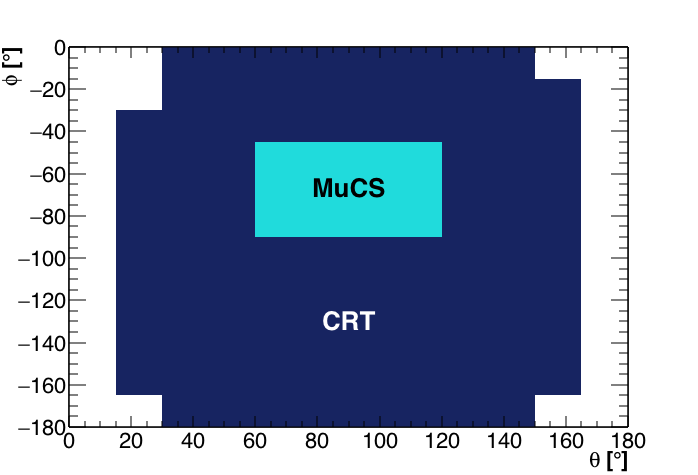
\includegraphics[width=0.7\linewidth]{figures/crt.png}
    \caption{Monte Carlo simulation of the coverage on the ($\theta,\phi$) plane of both the MuCS (light blue) and the CRT (dark blue).} \label{fig:crt}
  \end{center}
\end{figure}

\clearpage{}

\appendix
\section{Angular cuts}
In order to increase the purity of our sample it is possible to apply a cut on the difference between the extrapolated MuCS angles and the reconstructed track angles:
\begin{equation}
\Delta\theta = \theta_{\mathrm{MuCS}}-\theta_{\mathrm{reco}}, \quad \Delta\phi = \phi_{\mathrm{MuCS}}-\phi_{\mathrm{reco}}.
\end{equation}
In this way, reconstructed tracks closer than $d_{\mathrm{max}}$ but that do not correspond to a MuCS cosmic ray will have large $\Delta\theta$, $\Delta\phi$ values. $\Delta\theta$ and $\Delta\phi$ distributions, obtained with a MuCS Monte Carlo simulation, are plotted in Figure \ref{fig:res}.

\begin{figure}[htbp]
  \begin{subfigure}{0.5\textwidth}
    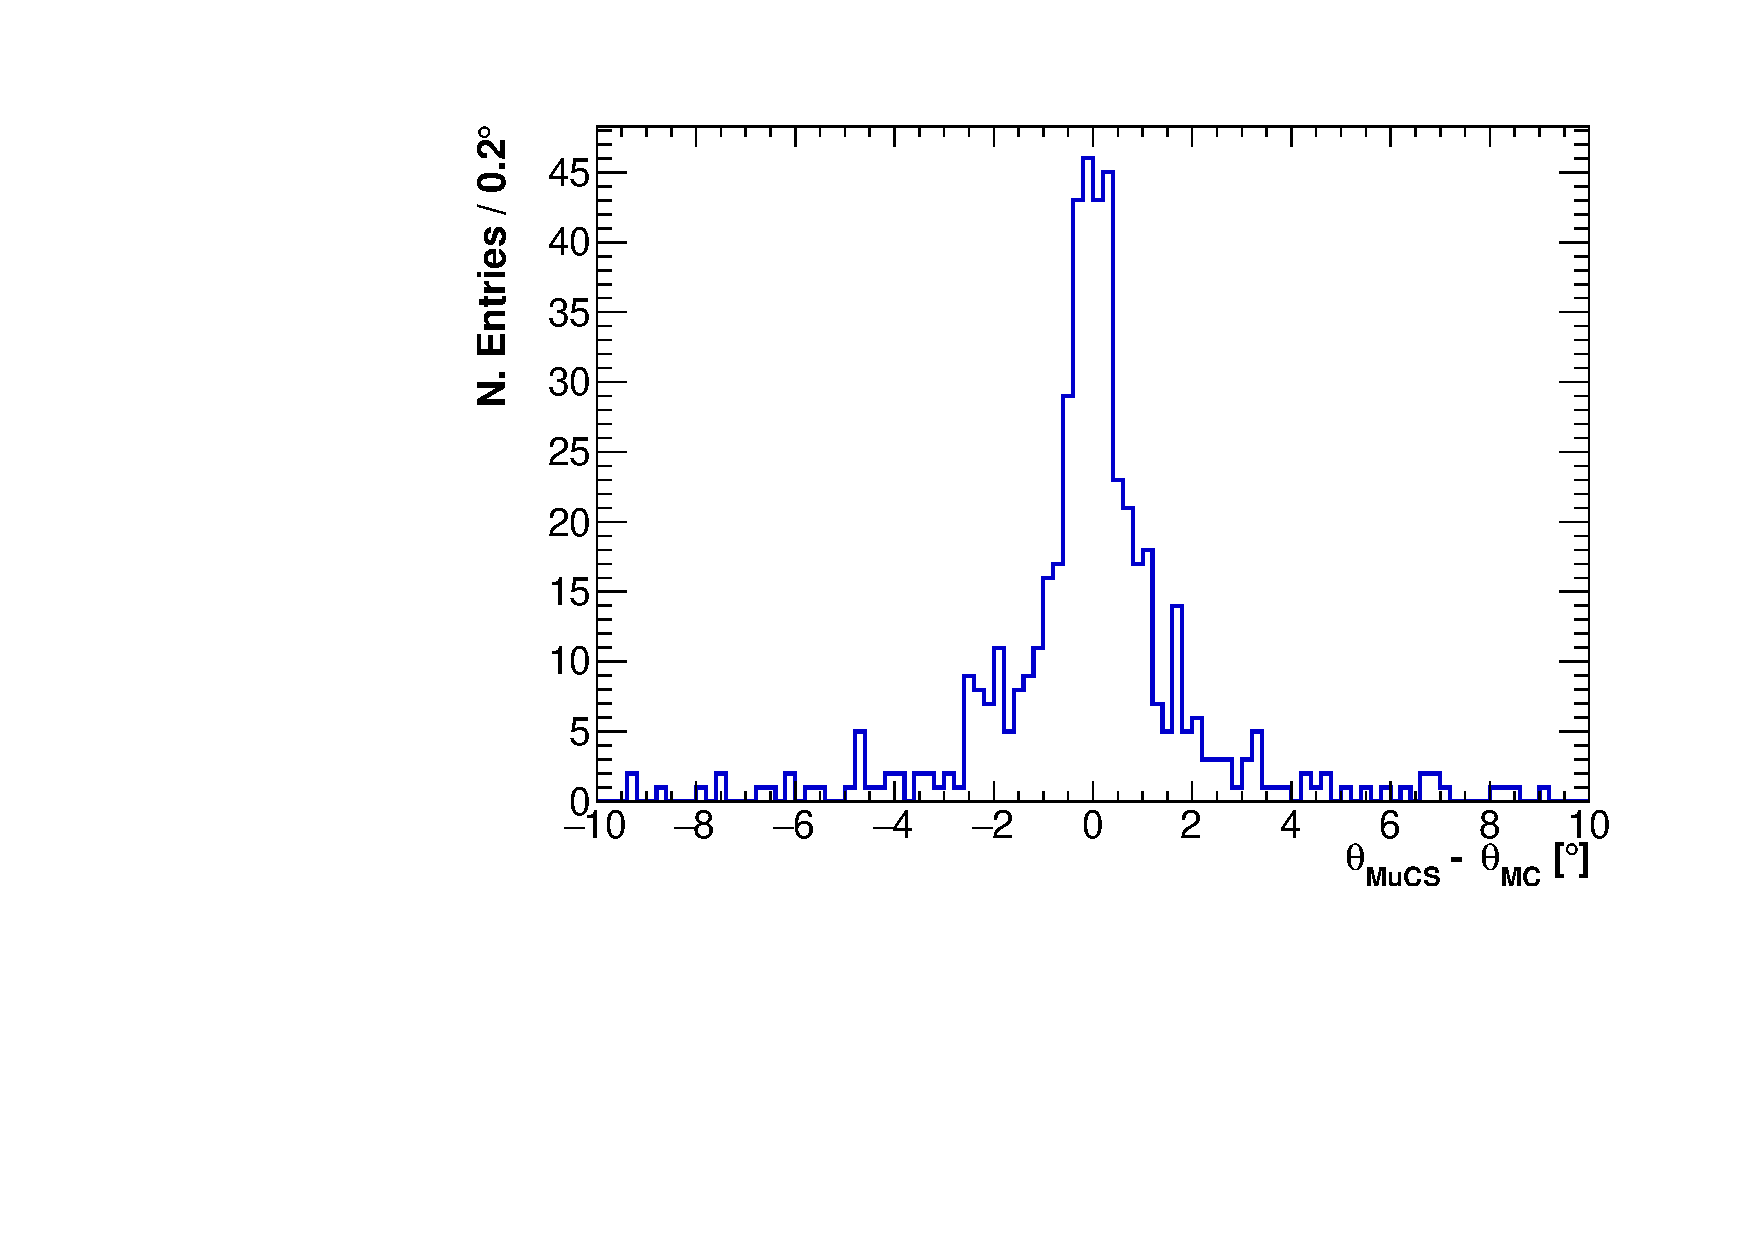
\includegraphics[width=\linewidth]{figures/theta_res.pdf}
    \caption{$\Delta\theta$}
  \end{subfigure}
  \begin{subfigure}{0.5\textwidth}
    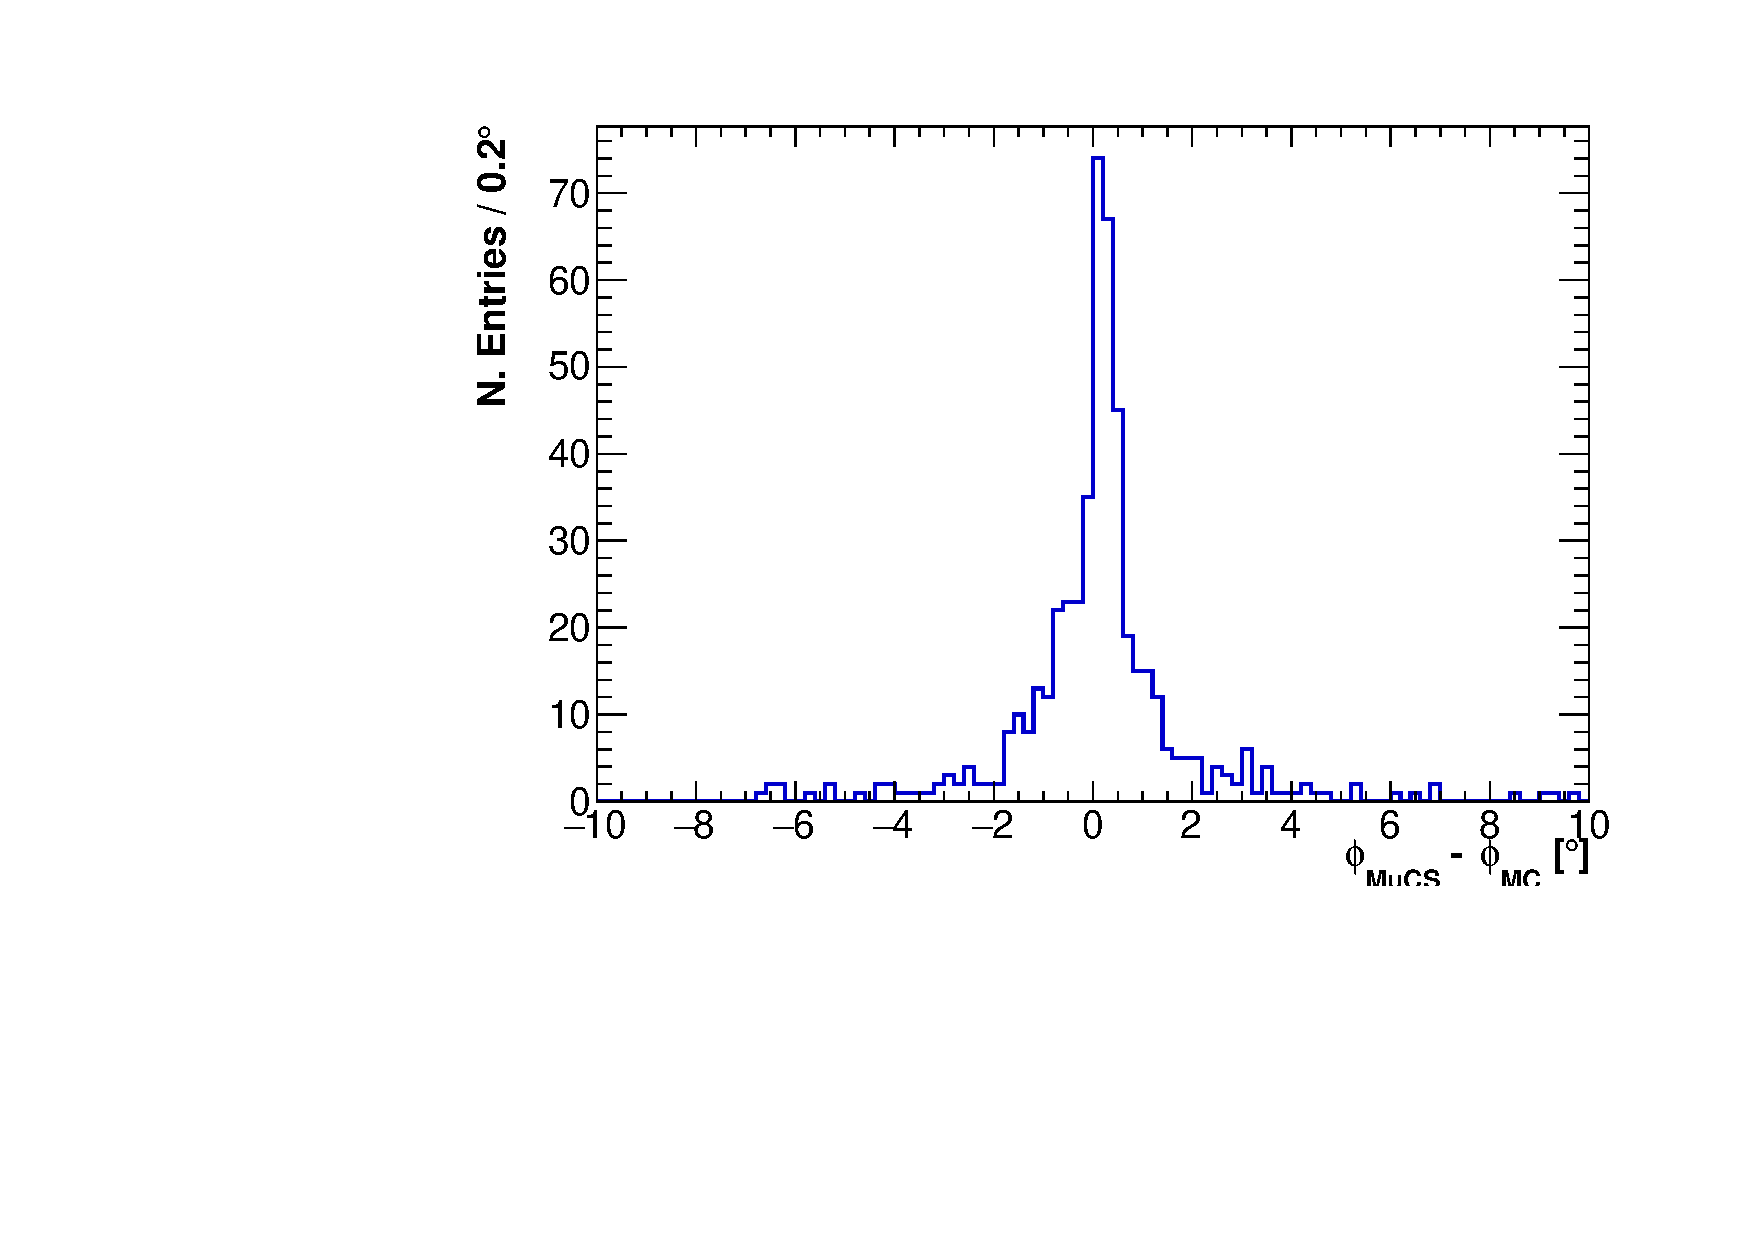
\includegraphics[width=\linewidth]{figures/phi_res.pdf}
    \caption{$\Delta\phi$}
  \end{subfigure}
\caption{Distribution of the difference between the extrapolated MuCS angles $\theta_{\mathrm{MuCS}}$, $\phi_{\mathrm{MuCS}}$ and the reconstructed angles $\theta_{\mathrm{reco}}$, $\phi_{\mathrm{reco}}$, obtained with a MuCS Monte Carlo simulation.}\label{fig:res}
\end{figure}

Selecting only the events with $|\Delta\theta| < 2^{\circ}$ and $|\Delta\phi| < 2^{\circ}$ increases the purity of the sample by 0.1\%. The effect of this cut has then been considered negligible.

\section{Technical details}
The datasets used in this analysis correspond to run 3702, for the central configuration, run 7347 for the downstream configuration and run 7702, 7703 for the upstream configuration. The reconstruction stages \texttt{reco1} and \texttt{reco2} use \texttt{uboonecode v05\_08\_00}. Their configuration is provided by the standard fcl files \texttt{reco\_uboone\_mcc7\_driver\_stage1.fcl} and \texttt{reco\_uboone\_mcc7\_driver\_stage2.fcl}. The source code of the \texttt{MuCSMerger} and \texttt{MuCSTagger} modules is available on the \texttt{uboonecode} repository.

The dataset with the merged MuCS and data information are stored in \texttt{/uboone/\allowbreak data/\allowbreak users/\allowbreak mibass/MuCS/MuCS/v05\_08\_00/MergedOuttree/}.
SAM dataset names for ArtRoot and anatree files are:
\begin{itemize}
  \item \texttt{MuCSRun3702\_Group158\_MuCSTaggedReco}(\texttt{\_ana}) for run 3702;
  \item \texttt{MuCSRun7347\_Group181\_MuCSTaggedReco}(\texttt{\_ana}) for run 7347;
  \item \texttt{MuCSRun7702\_Group182\_MuCSTaggedReco}(\texttt{\_ana}) for run 7702;
  \item \texttt{MuCSRun7703\_Group183\_MuCSTaggedReco}(\texttt{\_ana}) for run 7703.

\end{itemize}

\clearpage{}

\begin{thebibliography}{9}

  \bibitem{pandoracosmic} R. Acciarri, et al. [MicroBooNE Collaboration], \textit{The Pandora multi-algorithm approach to automated pattern recognition in LAr TPC detectors}. \texttt{MICROBOONE- NOTE-1015-PUB}, 2016. \url{http://www-microboone.fnal.gov/publications/publicnotes/index.html}.

  \bibitem{pandora} J.~S.~Marshall and M.~A.~Thomson, \textit{The Pandora Software Development Kit for Pattern Recognition}, Eur.\ Phys.\ J.\ C 75, no. 9, 439 (2015) \texttt{doi:10.1140/epjc/s10052\-015-3659-3} \texttt{[arXiv:1506.05348 [physics.data-an]]}.

  \bibitem{crt} M. Auger, et al., \textit{A Novel Cosmic Ray Tagger System for Liquid Argon TPC Neutrino Detectors}, submitted to Instruments, \texttt{arXiv:1612.04614 [physics.ins-det]}.

  \bibitem{mcdata} R. Acciarri, et al. [MicroBooNE Collaboration], \textit{A Comparison of Monte-Carlo Simulations and Data from MicroBooNE}, \texttt{MICROBOONE-NOTE-1014-PUB}, 2016. \url{http:// www-microboone.fnal.gov/publications/publicnotes/index.html}.

  \bibitem{cosmic} R. Acciarri, et al. [MicroBooNE Collaboration], \textit{Cosmic Shielding Studies at MicroBooNE}. \texttt{MICROBOONE-NOTE-1005-PUB}, 2016. \url{http:// www-microboone.fnal.gov/publications/publicnotes/index.html}.

  \bibitem{corsika} D.~Heck, et al.,
  \textit{CORSIKA: A Monte Carlo code to simulate extensive air showers},
  \texttt{FZKA-6019}, 1998.

  \bibitem{geant} S.~Agostinelli, et al. [GEANT4 Collaboration], \textit{GEANT4: A Simulation toolkit}, Nucl.\ Instrum.\ Meth.\ A {506}, 250 (2003).

  \bibitem{sce} R. Acciarri, et al. [MicroBooNE Collaboration], \textit{Space Charge Effect Measurements and Corrections}. \texttt{MICROBOONE-NOTE-1018-PUB}, 2016. \url{http: //www-microboone.fnal.gov/publications/publicnotes/index.html}.

  \bibitem{besiii} W.~L.~Yuan, et al., \textit{Study of tracking efficiency and its systematic uncertainty from $J/\psi \to p \overline{p} \pi^+ \pi^-$ at BESIII}, Chin.\ Phys.\ C 40 (2016) no.2,  026201 \texttt{doi:10.1088/1674-1137/40/2/026201 [arXiv:1507.03453 [hep-ex]]}.

  \bibitem{pdg} C.~Patrignani, et al. [Particle Data Group Collaboration], \textit{Review of Particle Physics}, Chin.\ Phys.\ C 40 (2016) no.10,  100001 \texttt{doi:10.1088/1674-1137/40/10/100001}.


\end{thebibliography}

\end{document}
